\let\mypdfximage\pdfximage
\def\pdfximage{\immediate\mypdfximage}
\documentclass[a4paper,12pt,default,numbered,print]{Classes_final/PhDThesisPSnPDF}


\ifsetMargin
\else
    \RequirePackage[left=37mm,right=30mm,top=35mm,bottom=30mm]{geometry}
    \setFancyHdr %
\fi


\ifsetFont
\else
    \RequirePackage{libertine} 
\fi





\ifsetBib %
\else %
    \RequirePackage[square, sort, numbers, authoryear]{natbib} %
\fi

\renewcommand{\bibname}{References}





\usepackage{setspace}
\linespread{1.5}






\RequirePackage[labelsep=space,tableposition=top]{caption} 
\renewcommand{\figurename}{Fig.} %








\usepackage{subcaption}
\usepackage{graphicx}




\usepackage{tabularx}
\usepackage{multirow}
\usepackage{booktabs}
\usepackage{makecell} %
\usepackage{colortbl}
\captionsetup[table]{font={stretch=1.1}}
\captionsetup[figure]{font={stretch=1.1}}

\usepackage{amsfonts}
\usepackage{amsmath}
\usepackage{amssymb}

\setcounter{secnumdepth}{2}
\setcounter{tocdepth}{2}

\usepackage{siunitx} %
\usepackage{xcolor}
\usepackage{float}
\renewcommand{\labelitemi}{$\bullet$}
\usepackage{gensymb} %
\usepackage{xspace}
\usepackage{rotating}
\usepackage{tikz}
\usepackage{tikz-3dplot}

\newcommand{\B}[1]{\textbf{#1}}

\newcommand{\Cref}[1]{Chapter~\ref{#1}}
\newcommand{\Tref}[1]{Table~\ref{#1}}
\newcommand{\eref}[1]{Eq.~\eqref{#1}}
\newcommand{\Eref}[1]{Equation~\eqref{#1}}
\newcommand{\fref}[1]{Fig.~\ref{#1}}
\newcommand{\Fref}[1]{Figure~\ref{#1}}
\newcommand{\Frefs}[1]{Figures~\ref{#1}}
\newcommand{\sref}[1]{Sec.~\ref{#1}}
\newcommand{\Sref}[1]{Section~\ref{#1}}

\newcommand{\argmax}{\mathop{\mathrm{argmax}}\limits}
\newcommand{\argmin}{\mathop{\mathrm{argmin}}\limits}
\newcommand{\rank}[1]{\mathsf{rank}\left(#1\right)}		%
\newcommand{\norm}[1]{\left\|#1\right\|}				%
\newcommand{\abs}[1]{\left\lvert#1\right\rvert}
\newcommand{\Span}[1]{\mathsf{span}\left\{#1\right\}}	%
\renewcommand{\dim}[1]{\mathsf{dim}\left(#1\right)}		%
\newcommand{\ran}[1]{\mathsf{ran}\left(#1\right)}		%
\newcommand{\Null}[1]{\mathsf{null}\left(#1\right)}		%
\newcommand{\V}[1]{\ensuremath{\mathbf{#1}}}

\def\eg{\emph{e.g}\onedot} \def\Eg{\emph{E.g}\onedot}
\def\ie{\emph{i.e}\onedot} \def\Ie{\emph{I.e}\onedot}
\def\cf{\emph{c.f}\onedot} \def\Cf{\emph{C.f}\onedot}
\def\etc{\emph{etc}\onedot} \def\vs{\emph{vs}\onedot}
\def\wrt{w.r.t\onedot} \def\dof{d.o.f\onedot}
\def\etal{\emph{et al}\onedot}

\newcommand{\vn}{\boldsymbol{n}}
\newcommand{\vv}{\boldsymbol{v}}
\newcommand{\vl}{\boldsymbol{l}}
\newcommand{\vM}{\mathbf{M}}
\newcommand{\vN}{\mathbf{N}}
\newcommand{\vL}{\mathbf{L}}
\newcommand{\vh}{\boldsymbol{h}}


\newcommand{\emphobject}[1]{\textsc{#1}\xspace} 
\newcommand{\PSFCNplusN}{PS-FCN$^{+\text{N}}$\xspace}
\newcommand{\diligent}{DiLiGenT benchmark\xspace}
\newcommand{\Diligent}{DiLiGenT Benchmark\xspace}
\newcommand{\lightstage}{Light Stage Data Gallery\xspace}
\newcommand{\gourd}{Gourd\&Apple dataset\xspace}
\newcommand{\dragonSVBRDF}{\emphobject{Dragon$^\text{SVBRDF}$}}
\newcommand{\syntestMERL}{SynTest$^\text{MERL}$\xspace}











\newcommand*{\MinNumber}{0}
\newcommand*{\MidNumber}{12} 
\newcommand*{\MaxNumber}{40}
\newcommand*{\Ratio}{70}

\usepackage{pgfplots}
\usepgfplotslibrary{dateplot}
\newcommand{\cl}[1]{%
        \ifdim #1 pt > \MidNumber pt
            \pgfmathsetmacro{\PercentColor}{max(min(\Ratio*(#1 - \MidNumber)/(\MaxNumber-\MidNumber),\Ratio),0.00)} %
            \edef\x{\noexpand\cellcolor{red!\PercentColor!yellow!80}}\x #1
        \else
            \pgfmathsetmacro{\PercentColor}{max(min(\Ratio*(\MidNumber - #1)/(\MidNumber-\MinNumber),\Ratio),0.00)} %
            \edef\x{\noexpand\cellcolor{green!\PercentColor!yellow!80}}\x #1
        \fi
}
\newcommand{\cla}[1]{#1}


\makeatletter
\DeclareRobustCommand\onedot{\futurelet\@let@token\@onedot}
\def\@onedot{\ifx\@let@token.\else.\null\fi\xspace}

\makeatother

\title{Single View Analysis of Non-Lambertian Objects Based on Deep Learning}
\author{Guanying Chen}
\dept{Department of Computer Science}
\university{The University of Hong Kong}
\crest{
\includegraphics[width=0.25\textwidth]{Classes_final/HKUcolour}}

\newcommand{\chinesename}{
\includegraphics[width=0.13\textwidth]{Classes_final/ChineseName_gy.pdf}}

\renewcommand{\submissiontext}{This dissertation is submitted for}
\degreename{Doctor of Philosophy}
\degreedate{December, 2020} 
\subject{Computer Vision} 
\keywords{{Computer Vision} {Image Matting} {Photometric Stereo} {Lighting Estimation} {Non-Lambertian}} 


\ifdefineAbstract
 \includeonly{Abstract/abstract} 
\else
\fi

\begin{document}
\frontmatter

\begin{titlepage}
\maketitle
\end{titlepage}

\newcommand{\gy}[1]{\textcolor{red}{[gy: #1]}}
\newcommand{\kywong}[1]{\textcolor{blue}{[kywong: #1]}}
\newcommand{\tred}[1]{\textcolor{red}{#1}}
\newcommand{\rev}[1]{\textcolor{red}{#1}}
\newcommand{\old}[1]{\textcolor{blue}{#1}}


\begin{dedication} 

To my parents.

\end{dedication}



\begin{declaration}

I hereby declare that except where specific reference is made to the work of others, the contents of this dissertation are original and have not been submitted in whole or in part for consideration for any other degree or qualification in this, or any other University. This dissertation is the result of my own work and includes nothing which is the outcome of work done in collaboration, except where specifically indicated in the text. 


\end{declaration}



\begin{acknowledgements}      
First, I would like to express my greatest gratitude to my supervisor, Dr.~Kwan-Yee Kenneth Wong, for his continuous support, thoughtful comments, and encouragement throughout my PhD study. Dr.~Wong's supervision helped me start my research in computer vision. I am very grateful for his efforts in both my research and life.

I was lucky to work with my collaborators, and would like to thank them for their invaluable advice and help:
Dr.~Kai Han for all my three projects (Chapter 1, Chapter 2, and part of Chapter 3);
Dr.~Boxin Shi and Prof.~Yasuyuki Matsushita for my second and third projects (Chapter 2 and Chapter 3);
Dr.~Michael Weather for my third project (part of Chapter 3).
In particular, part of my third project was done during my internship at Matsushita Lab in Osaka Univeristy, hosted by Prof.~Yasuyuki Matsushita.

I would like to show my sincere thanks to my colleagues and friends: Dr.~Xiaolong Zhu, Dr.~Xiao Tan, Dr.~Kai Han, Dr.~Wei Liu, Mr.~Chaofeng Chen, Mr.~Zhenfang Chen, Ms.~Jingjing Zhang, Ms.~Bingbin Liu, Mr.~Huiquan Zhou, and Ms.~Wenqi Yang, for their infectious enthusiasm in helping me in both studying and living.
    I also feel grateful for my friends Dr.~Miaomiao Liu, Dr.~Zhanghui Kuang, Dr.~Xuhui Jia, Dr.~Hao Zhou, Dr.~Xingdou Fu, Dr.~Guanbin Li, Dr. Zhen Li, Dr.~Weifeng Ge, and Dr.~Chaowei Fang.

In the summer of 2019, I was fortunate to have an internship at Matsushita Lab in Osaka University. I would like to thank Prof.~Yasuyuki Matsushita, Dr.~Michael Weather, Mr.~Heng Guo, Mr.~Xu Cao, Mr.~Feiran Li, Mr.~Hiroaki Santo, Mr.~Kenji Enomoto, and Mr.~Zhuoyu Yang for their help in both my research and living in Osaka.

I would like to express my heartfelt gratitude to The University of Hong Kong Foundation for Educational Development and Research (‘HKU Foundation’) for its generous support for my research studies in HKU.

Last, I want to thank my parents and beloved one Huijun Li for their unconditional love, support, and trust.

\end{acknowledgements}

\begin{abstract}
Non-Lambertian objects (\eg, transparent objects and specular objects) are very common in the real-world. However, existing computer vision algorithms developed for scene analysis often assume a Lambertian reflectance model, and treat non-Lambertian objects as outliers. It is important to develop robust methods for analysing non-Lambertian objects as it enables more complete and accurate understanding of the captured scene. This thesis tackles three vision problems of non-Lambertian objects under a single viewpoint, namely transparent object matting, calibrated photometric stereo, and uncalibrated photometric stereo for non-Lambertian objects.

The first part of this thesis addresses the problem of transparent object matting. Existing approaches often require tedious capturing procedures and long processing time, which limit their practical use. We formulate transparent object matting as a refractive flow estimation problem, and propose a deep learning framework, named \emph{TOM-Net}, for learning the refractive flow. At test time, TOM-Net takes a single image as input, and outputs a matte (consisting of an object mask, an attenuation mask and a refractive flow field) in a fast feed-forward pass. As no off-the-shelf dataset is available for transparent object matting, we create a large-scale synthetic dataset for training and capture a real dataset for testing. Besides, we show that our method can be easily extended to handle cases where a trimap or a background image is available.

The second part of this thesis addresses the problem of calibrated photometric stereo for non-Lambertian surfaces. Existing approaches often adopt simplified reflectance models to make the problem more tractable, but this greatly hinders their applications on real-world objects. We propose a deep fully convolutional network, named PS-FCN, that takes an arbitrary number of images of a static object captured under different light directions with a fixed camera as input, and predicts a normal map of the object in a fast feed-forward pass. Our method does not depend on a pre-defined set of light directions during training and testing.

The third part of this thesis considers the problem of uncalibrated photometric stereo, where light directions are unknown at test time. Specifically, we focus on estimating light directions from the input images, through which we cast the problem of uncalibrated photometric stereo into a calibrated one. We first introduce a novel convolutional network, named LCNet, to estimate light directions from input images. Unlike previous approaches that heavily rely on assumptions of specific reflectances and light source distributions, our method is able to determine light directions of a scene with unknown arbitrary reflectances observed under unknown varying light directions. We then analyse what had been learned by LCNet to resolve the ambiguity in lighting estimation. Inspired by our observations, we further introduce a guided calibration network (GCNet) to estimate more accurate lightings.
    ($446$ words)
\end{abstract}


\tableofcontents
\listoffigures
\listoftables 

\mainmatter



\chapter{Introduction}
\label{ch:intro}

\section{Motivation}
Over the past few decades, many algorithms have been developed for different vision problems, \eg, multi-view stereo~\cite{seitz2006comparison,agarwal2011building}, optical flow estimation~\cite{brox2004high,sun2014quantitative}, shape-from-shading~\cite{ikeuchi1981numerical,zhang1999shape}, image matting~\cite{smith1996blue,levin2007closed}, and photometric stereo~\cite{woodham1980ps,hayakawa1994photometric}.
However, these methods often rely on the assumption of a Lambertian surface, and treat the non-Lambertian objects (\eg, transparent and specular objects) as outliers. 

In fact, transparent and specular objects are very common in the real-world (\eg, glass, plastic, and metallic surfaces).
Simply treating them as outliers cannot thoroughly solve the underling problems.
It is important to develop robust methods for analyzing non-Lambertian objects as it enables a more complete and accurate understanding of the captured scene.

Different from a Lambertian surface whose observed brightness is the same from different viewing angles, the appearance of a non-Lambertian surface depends on how it interacts with the environment lights.
The appearance of a transparent object is determined by how it refracts, reflects, absorbs, and scatters the incident light. 
The appearance of a specular object is determined by how it reflects, absorbs, and scatters the incident light.
The complex interaction between the object and environment light increases the difficulties of analyzing transparent and specular objects.

Inspired by the great successes of deep learning based methods in various vision tasks~\cite{lecun1998gradient,krizhevsky2012imagenet,he2016deep}, we propose to take advantage of the powerful feature learning capability of convolutional neural networks (CNNs) and the large scale training data to solve the difficult problems involving non-Lambertian objects.
Specifically, in this thesis, we focus on three vision problems, namely transparent object matting, calibrated photometric stereo, and uncalibrated photometric stereo for non-Lambertian objects.

Traditional image matting methods are tailored for opaque objects. Given an input image, they estimate an object opacity for each pixel (\ie, alpha matte), then the foreground regions can be extracted and composited onto a novel background.
However, object opacity cannot model the refractive effect of a transparent object and thus leads to unrealistic composites (see~\fref{fig:intro_matting} for an example).
Existing methods for transparent object matting often require tedious capturing procedures and long processing time, which limit their practical use.
To address the limitation of the existing alpha matting methods, we introduce a simple and effective deep learning framework to tackle the problem of transparent object matting.

\begin{figure}[tbp] \centering
    \makebox[0.32\textwidth]{(a) Input image} 
    \makebox[0.32\textwidth]{(b) Composite result} 
    \makebox[0.32\textwidth]{(c) Photograph}
    \\
    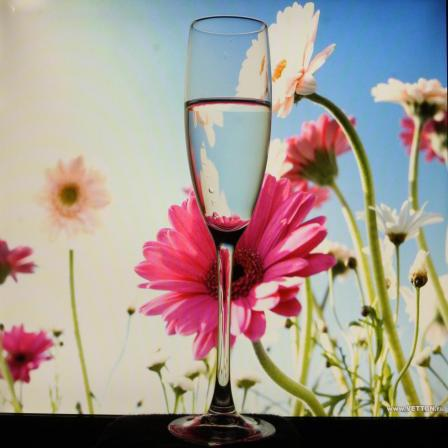
\includegraphics[width=0.32\textwidth]{ch-introduction/images/matting_input}
    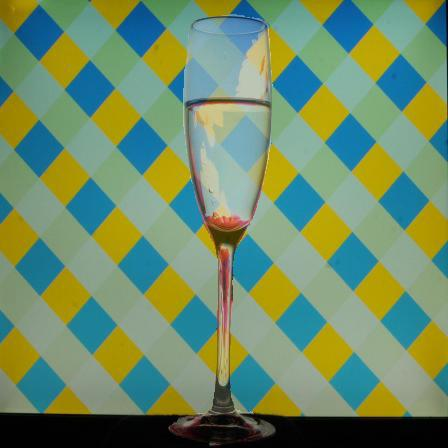
\includegraphics[width=0.32\textwidth]{ch-introduction/images/matting_output}
    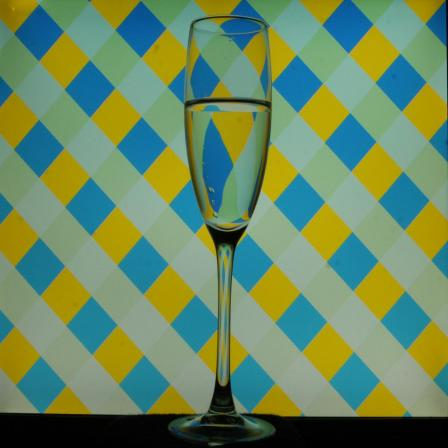
\includegraphics[width=0.32\textwidth]{ch-introduction/images/matting_ref}
    \caption[Example result of the traditional matting method for transparent object]{Example result of the traditional image matting method for transparent object. (a) Input image. (b) Composite result obtained by applying the estimated alpha matte on a novel background. (c) Captured photo of the transparent object in front of the novel background.} \label{fig:intro_matting}
\end{figure}

Photometric stereo aims at recovering the surface normal of a static object from a set of images captured under different light directions~\cite{woodham1980ps,silver1980determining} (see~\fref{fig:intro_ps}).
Compared with multi-view stereo methods, photometric stereo methods use monocular shading cues and naturally avoid the difficult correspondence problem. 
The advantage of photometric stereo is that it can handle specular and textureless surfaces, and can recover highly detailed scene geometry.
However, there are still some limitations in existing photometric stereo methods. (i) Traditional methods often adopt simplified reflectance models to simplify the problem, and this greatly hinders their applications to real-world objects. (ii) Photometric stereo methods typically require calibrated lightings, and the calibration process is often very tedious. There are a few works for uncalibrated photometric stereo, but their performances are far behind the calibrated ones.

In this thesis, we address both these two limitations of existing photometric stereo methods. 
First, we develop a flexible deep learning framework for calibrated photometric stereo. By directly learning a mapping from intensity observations to surface normal, our model can bypass the need for explicitly modeling the surface reflectance model of the object. 
Second, we develop a deep learning method to estimate light directions from the input images, through which we cast the problem of uncalibrated photometric stereo into a calibrated one.

\begin{figure} \centering
    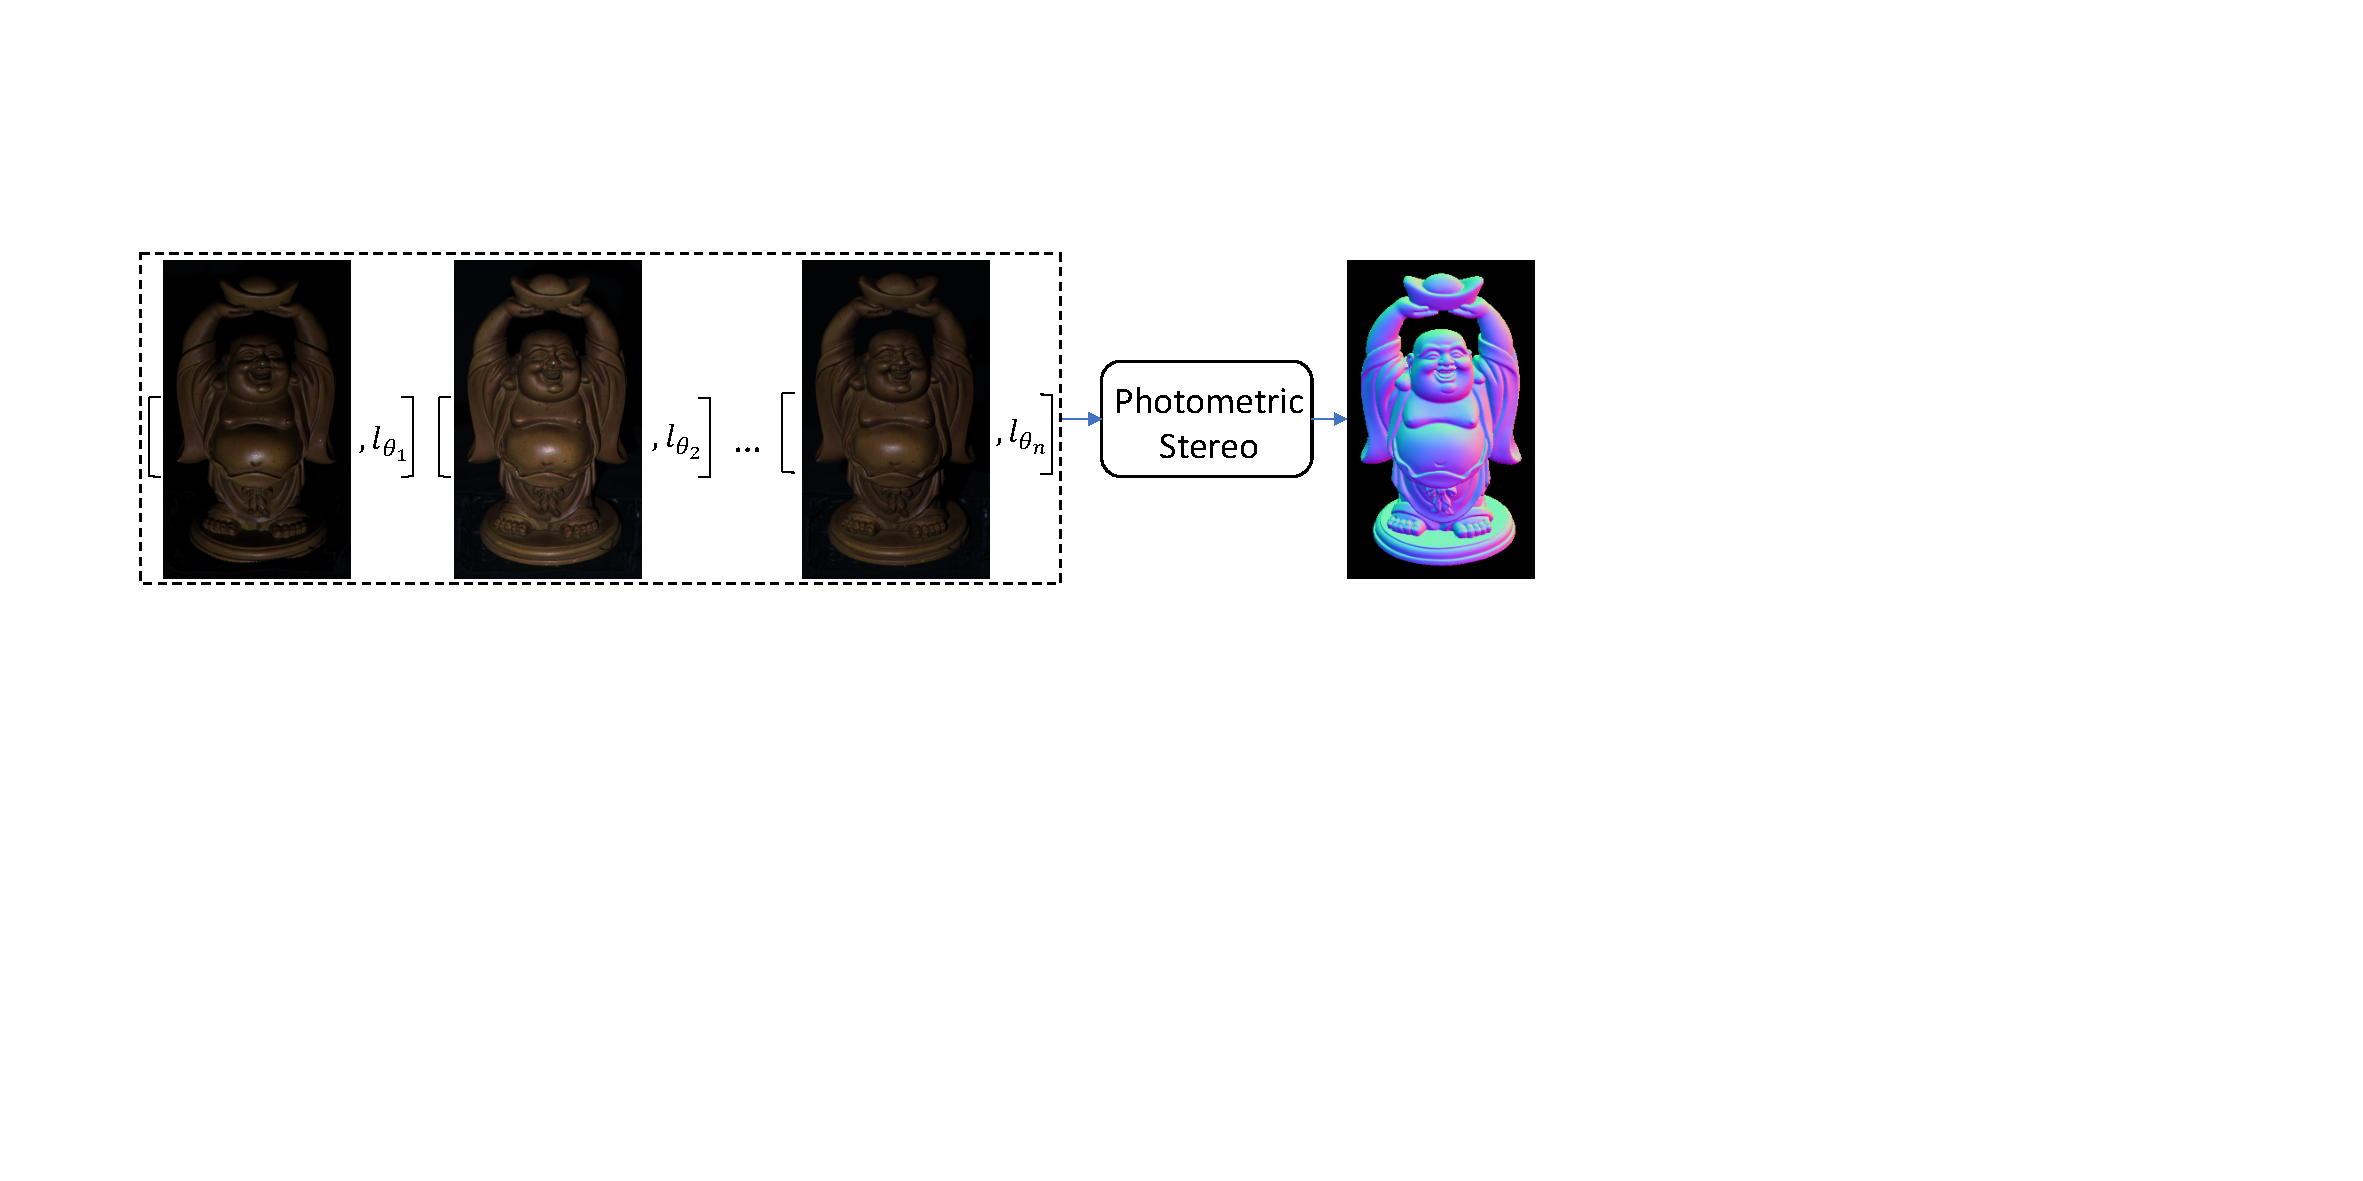
\includegraphics[width=\textwidth]{ch-introduction/images/Intro_PS}
    \caption[Illustration of photometric stereo]{Given multiple images of a static object captured under different light directions, photometric stereo can estimate a surface normal map of the object.} \label{fig:intro_ps}
\end{figure}


\section{Contributions}

The main contributions of this thesis can be summarized as follows:

\begin{itemize}
    \item a convolutional neural network for \textbf{transparent object matting from a single image}. We introduce a simple and efficient model for transparent object matting as simultaneous estimation of an object mask, an attenuation mask, and a refractive flow field. To train and evaluate the proposed method, we create a large-scale synthetic dataset and capture a real dataset as a benchmark for this problem. Preliminary results of this research have been published in~\cite{chen2018tomnet,chen2019learning}

    \item a flexible convolutional neural network for \textbf{calibrated photometric stereo}. Our method directly learns the mapping from reflectance observations to surface normals, and does not depend on a pre-defined set of light directions during training and testing. We introduce two synthetic datasets for learning photometric stereo. Our method outperforms existing methods on multiple real datasets, which demonstrates the effectiveness of the proposed method. Preliminary results of this research have been published in~\cite{chen2018ps,chen2020deepps}.
    \item a convolutional neural network for \textbf{estimating light directions for uncalibrated photometric stereo}. We analyze the features learned by our method, and find that attached shadows, shadings, and specular highlights are key elements for lighting estimation. Based on our findings, we propose an improved method that explicitly utilizes object shape and shading information as guidances for better lighting estimation. Preliminary results of this research have been published in~\cite{chen2019self,chen2020chen_gcnet}.
\end{itemize}

\section{Thesis Outline}
The remainder of this thesis is organized as follows.

\paragraph{\Cref{ch:tomnet}} This chapter addresses the problem of transparent object matting. Existing approaches often require tedious capturing procedures and long processing time, which limit their practical use. In this chapter, we formulate transparent object matting as a refractive flow estimation problem, and propose a deep learning framework, named {\em TOM-Net}, for learning the refractive flow. As no off-the-shelf dataset is available for transparent object matting, we introduce a large-scale synthetic dataset for training, and capture a real dataset for evaluation. 
We then show that our method can be extended to handle cases where a trimap or a background image is available. 
Promising experimental results have been achieved on both synthetic and real data, which clearly demonstrate the effectiveness of our approach.

\paragraph{\Cref{ch:psfcn}} This chapter addresses the problem of calibrated photometric stereo for non-Lambertian surfaces under directional lightings. Existing approaches often adopt simplified reflectance models to make the problem more tractable, but this greatly hinders their applications on real-world objects. 
We propose a deep fully convolutional network, named PS-FCN, that takes an arbitrary number of images of a static object captured under different light directions with a fixed camera as input, and predicts a normal map of the object in a fast feed-forward pass. 
As obtaining ground-truth normal maps of real objects is difficult and time-consuming, we introduce two realistic synthetic datasets for training.
Extensive experiments show that PS-FCN outperforms existing approaches in calibrated photometric stereo.

\paragraph{\Cref{ch:lcnet}} This chapter addresses the problem of lighting estimation for uncalibrated photometric stereo. Previous approaches for this problem often heavily rely on assumptions of specific reflectances and light source distributions.
We first introduce a lighting calibration network, named \emph{LCNet}, that takes an arbitrary number of images as input and estimates their corresponding light directions and intensities.
Surprised by the incredible effectiveness of LCNet, we analyze the features learned by this method and find that they strikingly resemble attached shadows, shadings, and specular highlights. Based on this insight, we propose a guided calibrated network, named \emph{GCNet}, that explicitly leverages object shape and shading information for improved lighting estimation.
Our experiments show that combining our network with existing calibrated photometric stereo methods yields significantly improved results over state-of-the-art uncalibrated methods. 

\paragraph{\Cref{ch:conclusion}} This chapter summarizes the theories and algorithms developed in this dissertation, followed by a brief discussion of potential future work.

\newcommand{\TOMNetTrimap}{TOM-Net$^{\text{+Trimap}}$\xspace}
\newcommand{\TOMNetBg}{TOM-Net$^{\text{+Bg}}$\xspace}
\chapter{Learning Transparent Object Matting}
\label{ch:tomnet}

\section{Introduction}
Image matting refers to the process of extracting the foreground matte of an image by locating the region of the foreground object and estimating the opacity of each pixel inside the foreground region. The foreground object can then be composited onto a new background image using the \emph{matting equation}~\cite{smith1996blue} 
\begin{equation}
    \label{eq:alphamatte}
    C = F + (1-\alpha)B,  \quad \alpha \in [0, 1],
\end{equation}
where $C$ denotes the composited color, $F$ the foreground color, $B$ the background color, and $\alpha$ the opacity.

Image matting has been widely used in image editing and film production. However, most of the existing methods are tailored for opaque objects, and cannot handle transparent objects whose appearance depends on how light is refracted from the background.

To model the effect of refraction, Zongker~\etal~\cite{zongker1999environment} introduced \emph{environment matting} as 
\begin{equation}
    \label{eq:em_general}
    C = F + (1-\alpha)B + \Phi, \quad \alpha \in [0, 1],
\end{equation}
where $\Phi$ is the contribution of environment light caused by refraction or reflection at the foreground object. Besides estimating the foreground shape, environment matting also describes how objects interact with the background. 

\begin{figure}[t] \centering
    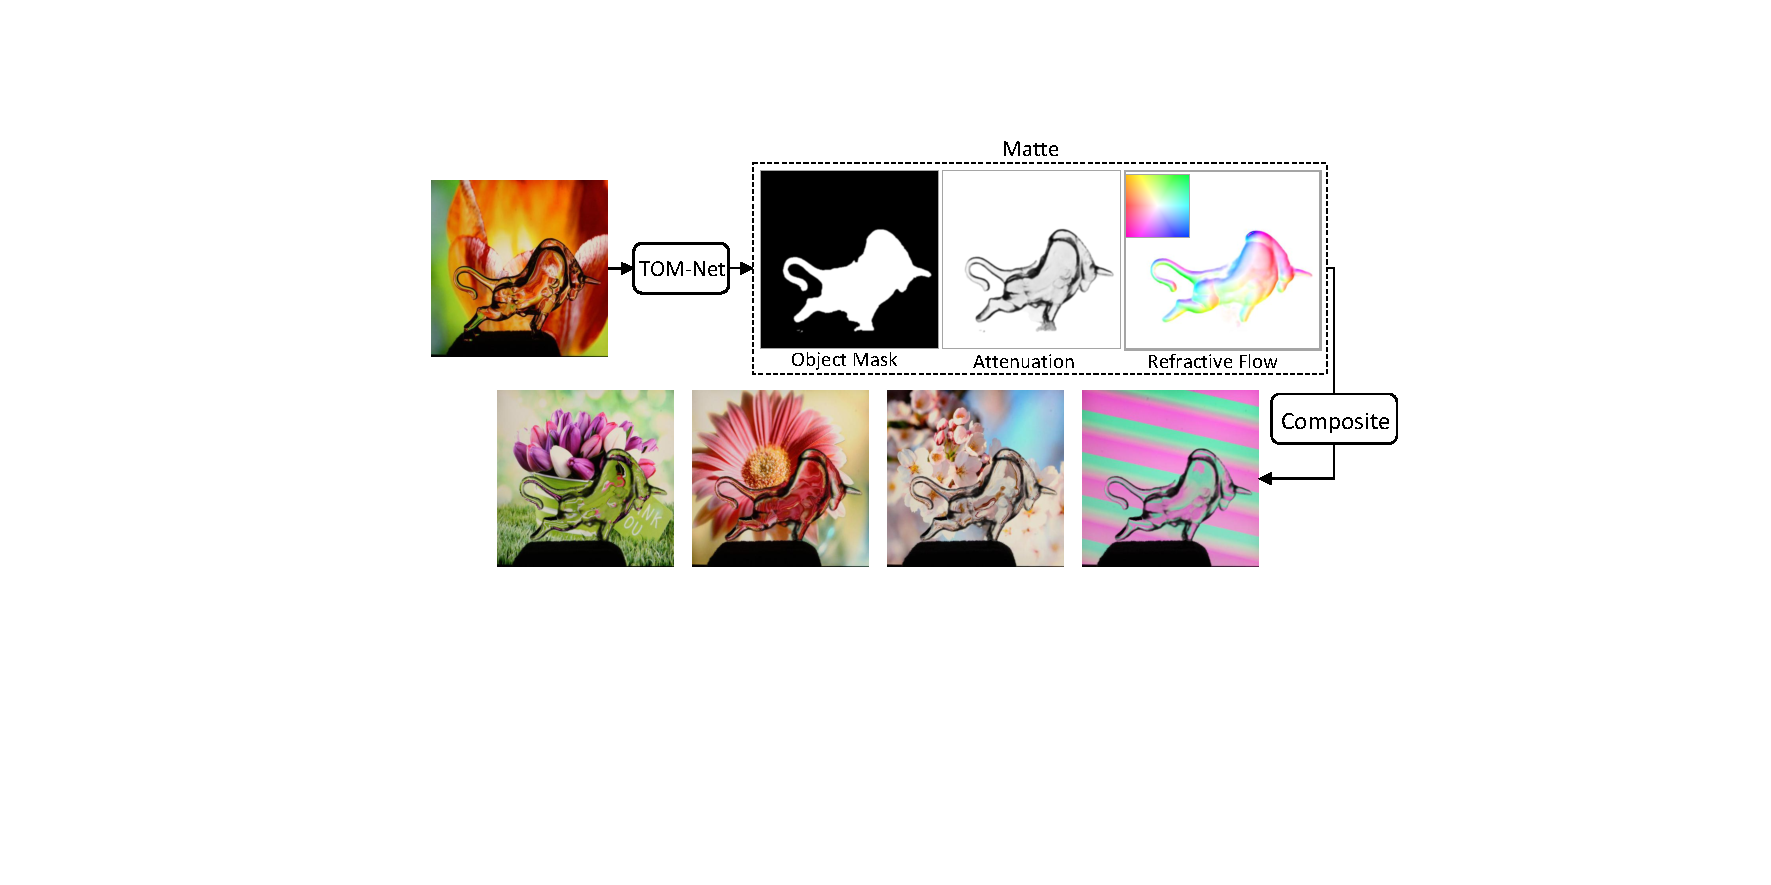
\includegraphics[width=\textwidth]{ch-tomnet/images/Method/Intro_network_intro_v3}
    \caption[Learning transparent object matting]{Learning transparent object matting. Given an image of a transparent object as input, our model can estimate the environment matte (consisting of an object mask, an attenuation mask, and a refractive flow field) in a feed-forward pass. The transparent object can then be composited onto new background images with the extracted matte.}
    \label{fig:intro}
\end{figure}

Many efforts~\cite{chuang2000environment,wexler2002image,peers2003wavelet,zhu2004frequency,duan2011flexible,duan2015compressive} have been devoted to improving the seminal work of~\cite{zongker1999environment}. The resulting methods often require either a huge number of input images to achieve a higher accuracy, or the use of specially designed patterns to reduce the number of required images. They are in general all very computational expensive.

In this work, we focus on environment matting for transparent objects. It is highly ill-posed, if not impossible, to estimate an accurate environment matte for transparent objects from a single image with an arbitrary background. Given the huge solution space, there exist multiple objects and backgrounds which can produce the same refractive effect. In order to make the problem more tractable, we simplify our problem to estimating an environment matte that can produce visually realistic refractive effect from a single image, instead of estimating a highly accurate refractive flow. We define the environment matte in our model as a triplet consisting of an object mask, an attenuation mask, and a refractive flow field. Realistic refractive effect can then be obtained by compositing the transparent object onto new background images (see \fref{fig:intro}). We then show that the performance of the proposed method can be improved when a trimap or a background image is available.

Inspired by the great successes of convolutional neural networks (CNNs) in high-level computer vision tasks, we propose a convolutional neural network, called TOM-Net, for simultaneous learning of an object mask, an attenuation mask, and a refractive flow field from a single image with an arbitrary background. The key contributions of this work can be summarized as follows:

\begin{itemize}
  \item We introduce a simple and efficient model for transparent object matting as simultaneous estimation of an object mask, an attenuation mask, and a refractive flow field.
  \item We propose a convolutional neural network, TOM-Net, to learn an environment matte of a transparent object from a single image. To the best of our knowledge, TOM-Net is the first CNN that is capable of learning transparent object matting.
  \item We create a large-scale synthetic dataset and a real dataset as a benchmark for learning transparent object matting. Our TOM-Net has produced promising results on both the synthetic and real datasets.
  \item We propose two additional convolutional neural networks, denoted as \TOMNetTrimap and \TOMNetBg, for handling the cases where a trimap or a background image is available, respectively.
\end{itemize}  

Preliminary results of this chapter were published in~\cite{chen2018tomnet,chen2019learning}.
Our code, trained models, and datasets can be found at \url{https://guanyingc.github.io/TOM-Net}.

\section{Related Work}
\label{sec:related_work}
In this section, we briefly review representative works on environment matting and recent works on CNN based image matting. 

\paragraph{Environment matting}
\label{par:Environment Matting}
Zongker~\etal~\cite{zongker1999environment} introduced the concept of environment matting, and assumed each foreground pixel being originated from a single rectangular region of the background. They obtained the environment matte by identifying the corresponding background region for each foreground pixel using three monitors and multiple images. Chuang~\etal~\cite{chuang2000environment} extended~\cite{zongker1999environment} in two different ways. First, they replaced the single rectangular supporting area for a foreground pixel with multiple 2D oriented Gaussian strips. This makes it possible for their method to model the effects of color dispersion, multiple mapping, and glossy reflection. Second, they simplified the environment matting equation by assuming the object being colorless and perfectly transparent. This allows them to achieve real time capture environment matting (RTCEM). The environment matte was then extracted with one image taken in front of a pre-designed pattern. However, RTCEM requires background images to segment the transparent objects, and depends on a time-consuming off-line processing. 

Wexler~\etal~\cite{wexler2002image} introduced a probabilistic model based method which assumes each background point has a probability to make contribution towards the color of a certain foreground point. Their approach does not require pre-designed patterns during data acquisition, but it still needs multiple images and can only model thin transparent objects. Peers and Dutr{\'e}~\cite{peers2003wavelet} used a large number of wavelet basis backgrounds to obtain the environment matte, and their method can also model the effect of diffuse reflection. Based on the fact that a signal can be decomposed uniquely in the frequency domain, Zhu and Yang~\cite{zhu2004frequency} proposed a frequency-based approach to extract an accurate environment matte. They used Fourier analysis to solve the decomposition problem. Both~\cite{peers2003wavelet} and~\cite{zhu2004frequency} require a large number of images to extract the matte (\eg,~\cite{peers2003wavelet} needs $2,400$ images and~\cite{zhu2004frequency} needs $4,096$ images for an image of size $1024\times 1024$), making them not very practical. Recently, compressive sensing theory has been applied to environment matting to reduce the number of images required. Duan~\etal~\cite{duan2011fast} applied this theory in  the spatial domain and Qian~\etal~\cite{qian2015frequency} applied it in the frequency domain. However, the number of images needed is still in the order of hundreds. In contrast, our work can estimate an environment matte from a single image in a fast feed-forward computation without the need for pre-designed patterns or additional background images.

\begin{sidewaystable}[htbp]
    \caption[Comparison of different environment matting methods]{Comparison of different environment matting methods. $k$ indicates the image size and mapping type stands for how a foreground point is composited by the point(s) in the background image.}
    \label{tab:related_work}
        \resizebox{\textwidth}{!}{
    \Large
    \begin{tabular}{lllllcc}
        \toprule
        \textbf{Methods} & \makecell{\textbf{Asymptotic} \\ \textbf{\# images}}  & \makecell{\textbf{\# images} \\($k=1024)$} & \makecell{\textbf{Typical runtime}\\($k=1024$)} & \textbf{Mapping type} & \textbf{Materials} & \textbf{Remarks} \\
        \midrule
        Ours                                         & $O(1)$  & $1$              & \makecell{$0.5$ secs when $k=512$ \\ (run on a GPU)} & single-pixel & colorless, specularly refractive & \makecell{aims for visually realistic effect} \\
        \midrule                                                                    
RTCEM \cite{chuang2000environment}                    & $O(1)$  & $1$              & $2$ mins & single-pixel & colorless, specularly refractive & \makecell{requires a coded background \\ and off-line processing}\\
        \midrule                                                                    
Yeung et. al \cite{yeung2011matting}                 & $O(1)$  & $1$              & $30$ secs & single-pixel & colored refractive  & \makecell{requires human interaction, \\ aims for visually realistic effect}\\
        \midrule                                                                    
Zongker \textit{et al}. \cite{zongker1999environment}& $O(\log k)$ & $20$         & $20$ mins when $k=512$& single-region & \makecell{colored refractive, translucent, \\ highly specular} & assumes rectangular support region \\
        \midrule                                                                    
Chuang \textit{et al}. \cite{chuang2000environment}  & $O(k)$ & $1800$             & not available & multi-region & \makecell{Zongker \textit{et al}. \cite{zongker1999environment} + (color dispersion, \\ multiple mapping, glossy reflection)} & \makecell{requires solving a complex \\ optimization problem}\\
        \midrule                                                                    
Wavelet \cite{wang2004image}                         & $O(k)$ & $ 2400$            & $12$ hours & multi-region&  same as Chuang \textit{et al}. \cite{chuang2000environment} & runtime includes data acquisition \\
        \midrule                                                                    
Frequency \cite{zhu2004frequency}                    & $O(k)$ & $ 4096$            & $5-10$ mins & multi-pixel & \makecell{Zongker \textit{et al}. \cite{zongker1999environment} + (color dispersion, \\ glossy reflection)} & slow data acquisition   \\
        \midrule                                                                    
Duan \textit{et al}. \cite{duan2011fast}             & $O(s\log (k^2/s))$ & $ 340$ & $2.8$ mins & multi-region&  same as Chuang \textit{et al}. \cite{chuang2000environment} & $s$ denotes the sparsity of a signal \\ %
        \midrule                                                                    
Qian \textit{et al}. \cite{qian2015frequency}        & $O(s\log (2k/s))$ & $ 400$  & $3.3$ mins & multi-pixel & same as Frequency \cite{zhu2004frequency} & $s$ denotes the sparsity of a signal\\
        \bottomrule
    \end{tabular}
    }


\end{sidewaystable}

Yeung~\etal~\cite{yeung2011matting} proposed an interactive way to estimate an environment matte given an image containing a transparent object. Their method requires users to manually mark the foreground and background in the image, and models the refractive effect using a thin-plate-spline transformation. Their method does not produce an accurate environment matte, but instead a visually pleasing refractive effect. Our method shares the same spirit, but does not involve any human interaction. 

\Tref{tab:related_work} shows a comparison of different environment matting methods. Compared with other methods, our method requires only a single image and can extract a matte in $0.5$ second without the need for any predefined backgrounds.

\paragraph{CNN based image matting}
Although the potential of CNN on transparent object matting has not yet been explored, some existing work have adopted CNNs for solving the traditional image matting problem. Shen~\etal~\cite{shen2016deep} introduced a CNN for image matting of color portrait images. Cho~\etal~\cite{cho2016natural} proposed a network to predict a better alpha matte by taking the matting results of the traditional method and normalized color images as input. 
Some deep learning methods~\cite{xu2017deep,zhang2019late,lu2019indices} have been introduced to estimate an alpha matte given an image and its trimap. 
However, none of these methods can be applied directly to the task of transparent object matting as object opacity alone is not sufficient to model the refractive effect. 

\section{Matting Formulation}
\label{sec:formulation}
As a transparent object may have multiple optical properties (\eg, color attenuation, translucency, and reflection), estimating an accurate environment matte for a generic transparent object from a single image is very challenging. 
Following the work of~\cite{chuang2000environment}, we cast environment matting to a refractive flow estimation problem by assuming that each foreground pixel only originates from one point in the background due to refraction. Compared to the seminal work of~\cite{zongker1999environment}, which models each foreground pixel as a linear combination of a patch in the background, our formulation is more tractable and can be easily encoded using a CNN.

In~\cite{zongker1999environment}, the per-pixel environment matting is obtained through leveraging color information from multiple background images. Given a set of pre-designed background patterns, matting is formulated as
\begin{equation}
    \label{eq:em_origin}
    C = F + (1-\alpha)B + \sum_{i=1}^{k} R_i \mathcal{M}(\mathbf{T}_i, \mathbf{A}_i),
\end{equation}
where $F$, $B$ and $\alpha$ denote the ambient illumination, background color and opacity, respectively. The last term in \eref{eq:em_origin} accounts for the environment light accumulated from $k$ pre-designed background images ($k=3$ in~\cite{zongker1999environment}). $R_i$ is a factor describing the contribution of light emanating from the $i$-$th$ background image $\mathbf{T}_i$. $\mathcal{M}(\mathbf{T}_i, \mathbf{A}_i)$ denotes the average color of a rectangular region $\mathbf{A}_i$ on the background image $\mathbf{T}_i$. 

To obtain an environment matte, the transparent object is placed in front of the monitor(s), and multiple pictures of the object are captured with the monitor(s) displaying different background patterns\footnote{For an image of size $512\times 512$, $18$ pictures and around $20$ minutes processing time are needed.}. 
Generally, a surface point receives light from multiple directions, especially for a diffuse surface. When it comes to a perfectly transparent object, however, a surface point will only receive light from one direction as determined by the law of refraction. Consider a single background image as the only light source (\ie, no ambient illumination), the problem can be modeled as
\begin{equation}
    \label{eq:em_simplify1}
    C = (1-\alpha)B + R \mathcal{M}(\mathbf{T}, P),
\end{equation}
where $\mathcal{M}(\mathbf{T}, P)$ is a bilinear sampling operation at location $P$ on the background image $\mathbf{T}$. Further, by assuming a colorless transparent object, $R$ becomes a  light attenuation index $\rho$ (a scalar value). The formulation in \eref{eq:em_simplify1} can be simplified to
\begin{equation}
    \label{eq:em_simplify2}
    C = (1-\alpha)B + \rho \mathcal{M}(\mathbf{T}, P),
\end{equation}
where $\rho \in [0, 1]$ denotes the attenuation index.

Here, we use refractive flow to model the refractive effect of a transparent object. The refractive flow of a foreground pixel is defined as the offset between the foreground pixel and its refraction correspondence on the background image. 

We further introduce a binary foreground mask to define the object region in the image. The matting equation can now be rewritten as
\begin{equation}
    \label{eq:em_simplify3}
    C = (1 - m) B + m\rho \mathcal{M}(\mathbf{T}, P),
\end{equation}
where $m \in\{0, 1\}$ denotes background ($m = 0$) or foreground ($m = 1$). The matte can then be estimated by solving $m$, $\rho$ and $P$ for each pixel in the input image containing the transparent 
object\footnote{For an image with $n$ pixel, we have $7$ unknowns ($3$ for $B$, $2$ for $P$, $1$ for $m$, and $1$ for $\rho$) for each pixel, resulting in a total of $7n$ unknowns.}.


\section{Learning Transparent Object Matting}
\label{sec:method}
In this section, we present a two-stage deep learning framework, called TOM-Net, for learning transparent object matting (see \fref{fig:networkStructure}). The first stage, denoted as CoarseNet, is a multi-scale encoder-decoder network that takes a single image as input, and predicts an object mask, an attenuation mask, and a refractive flow field simultaneously. CoarseNet is capable of predicting a robust object mask. However, the estimated attenuation mask and refractive flow field lack local structural details. 
To overcome this problem, we introduce the second stage of TOM-Net, denoted as RefineNet, to achieve a sharper attenuation mask and a more detailed refractive flow field. RefineNet is a residual network~\cite{he2016deep} that takes both the input image and the output of CoarseNet as input. After training, our TOM-Net can predict an environment matte from a single image in a fast feed-forward pass.

\begin{figure}[tbp] \centering
    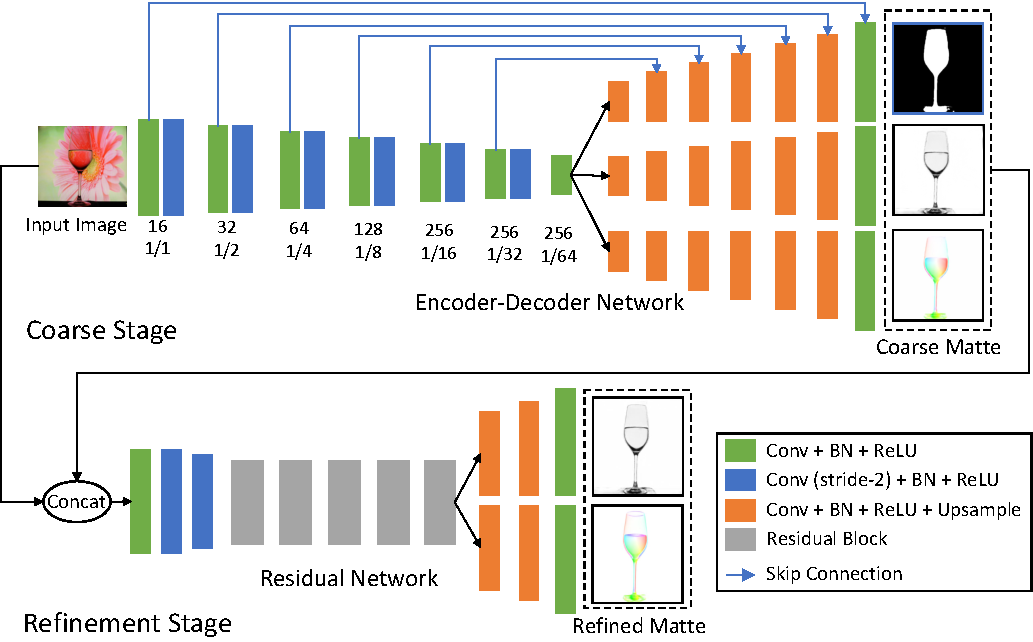
\includegraphics[width=\textwidth]{ch-tomnet/images/Method/TOMNet_framework.pdf}
    \caption[Network architecture of TOM-Net]{Network architecture of TOM-Net. The upper subnetwork is the CoarseNet and the bottom subnetwork is the RefineNet. (Cross-link and multi-scale outputs are not shown for simplicity.)} \label{fig:networkStructure}
\end{figure}

\subsection{Encoder-Decoder for Coarse Prediction}
\label{sub:Encoder-decoder Net for Coarse Prediction}
The first stage of our TOM-Net (\ie, CoarseNet) is based on mirror-link CNN introduced in~\cite{shi2016learning}. Mirror-link CNN was proposed to learn non-Lambertian object intrinsic decomposition. Its output consists of an albedo map, a shading map, and a specular map. It shares a similar output structure with our transparent object matting task (\ie, three output branches sharing the same spatial dimensionality). Therefore, it is reasonable for us to adapt mirror-link CNN for our CoarseNet. 

The mirror-link CNN adapted for our CoarseNet consists of one shared encoder and three distinct decoders. The encoder contains six down-sampling convolutional blocks, leading to a down-sampling factor of $64$ in the bottleneck layer. Features in the encoder layers are connected to the decoder layers having the same spatial dimensions through skip connections~\cite{ronneberger2015u}. Cross-links~\cite{shi2016learning} are introduced to make different decoders share the same input in each layer, so that decoders can better utilize the correlation between different predictions.

Learning with multi-scale loss has been proven to be helpful in dense prediction tasks (\eg,~\cite{eigen2014depth,fischer2015flownet}). Since we formulate the problem of transparent object matting as refractive flow estimation, which is a dense prediction task, we augment our mirror-link CNN with multi-scale loss similar to~\cite{fischer2015flownet}. 
We use four different scales in our model, where the first scale starts from the decoder features with a down-sampling factor of $8$ and the largest scale has the same spatial dimensions as the input.

In contrast to the recent two-stage framework for image matting~\cite{xu2017deep}, our TOM-Net has a shared encoder and three parallel decoders to accommodate different outputs. Besides, we augment our CoarseNet with multi-scale loss and cross-link. Moreover, TOM-Net is trained from scratch while the encoder in~\cite{xu2017deep} is initialized with the pre-trained VGG16.

\newcommand{\mathL}{\mathcal{L}}
\subsection{Loss Function for Coarse Stage}
\label{sub:Loss Function for CoarseNet}
CoarseNet takes a single image as input and predicts the environment matte as a triplet consisting of an object mask, an attenuation mask, and a refractive flow field. The learning of CoarseNet is supervised by the ground-truth matte using an object \textbf{m}ask \textbf{s}egmentation loss $\mathL_{ms}$, an \textbf{a}ttenuation \textbf{r}egression loss $\mathL_{ar}$, and a refractive \textbf{f}low \textbf{r}egression loss $\mathL_{fr}$. Besides, the predicted matte is expected to render an image as close to the input image as possible when applied to the ground-truth background based on \eref{eq:em_simplify3}. Hence, in addition to the supervision of the matte, we also take \textbf{i}mage \textbf{r}econstruction loss $\mathL_{ir}$ into account (bilinear sampling is implemented following~\cite{jaderberg2015spatial}). Note that the ground-truth background is only used to calculate the reconstruction error during training but not needed during testing. CoarseNet can therefore be trained by minimizing 
\begin{align}
    \mathL^c = \alpha^c_{ms} \mathL_{ms} + \alpha^c_{ar} \mathL_{ar} + \alpha^c_{fr} \mathL_{fr} + \alpha^c_{ir} \mathL_{ir},
\end{align}
where 
$\alpha^c_{ms}, \alpha^c_{ar}, \alpha^c_{fr}, \alpha^c_{ir}$ are weights for the corresponding loss terms. 

\paragraph{Object mask segmentation loss}
\label{par:Object Mask Classification Loss}
Object mask segmentation is simply a spatial binary classification problem. The output of the object mask decoder has a dimension of $2\times H\times W$, where $H$ and $W$ denote the height and width of the input. We normalize the output with {\em softmax} and compute the loss using the binary cross-entropy function
\begin{equation}
    \mathL_{ms} = -\frac{1}{HW} \sum_{ij} (\tilde{M}_{ij}\log(P_{ij}) + (1-\tilde{M}_{ij}) \log(1-P_{ij})),
\end{equation}
where $\tilde{M}_{ij} \in \{0,1\}$ and $P_{ij}\in [0,1]$ represent ground truth and normalized foreground probability of the pixel at $(i, j)$, respectively.

\paragraph{Attenuation regression loss} 
The predicted attenuation mask has a dimension of  $1\times H\times W$. The value of this mask is in the range of $[0, 1]$, where $0$ indicates no light can pass and $1$ indicates the light will not be attenuated. 
We adopt a mean square error (MSE) loss
\begin{equation}
    \mathL_{ar} = \frac{1}{HW} \sum_{ij} (A_{ij}-\tilde{A}_{ij})^2,
\end{equation}
where $A_{ij}$ is the predicted attenuation index and $\tilde{A}_{ij}$ the ground truth at $(i, j)$.
\paragraph{Refractive flow regression loss}
\label{par:Disparity Smoothness Loss}
The predicted refractive flow field has a dimension of $2\times H\times W$, where we have one channel for the horizontal displacement and another for the vertical displacement. We normalize the refractive flow with $tanh$ activation and multiply it by the width of the input, such that the output is constrained in the range of $[-W, W]$.
We adopt an average end-point error (EPE) loss
\begin{equation}
    \mathL_{fr} = \frac{1}{HW} \sum_{ij} \sqrt{(F^x_{ij}-\tilde{F}^x_{ij})^2 + (F^y_{ij}-\tilde{F}^y_{ij})^2},
\end{equation}
where $(F^x, F^y)$ and $(\tilde{F}^x, \tilde{F}^y)$ denote the predicted flow and the ground truth, respectively.

\paragraph{Image reconstruction loss}
\label{par:Image Reconstruction Loss}
We use MSE loss to measure the dissimilarity between the reconstructed image and the input image. 
Denoting the reconstructed image by $I$ and the ground-truth image (\ie, the input image) by $\tilde{I}$, the reconstruction loss is given by
\begin{equation}
    \mathL_{ir} = \frac{1}{HW} \sum_{ij} \Vert I_{ij}-\tilde{I}_{ij}\Vert_2^2.
\end{equation}

\paragraph{Implementation details}
\label{par:Implementation Details}
In all experiments, we empirically set $\alpha^c_{ms}=0.1, \alpha^c_{ar}=1, \alpha^c_{fr}=0.01,$ and $\alpha^c_{ir}=1$. The loss weights for different scales are $\frac{1}{2^{(4 -\text{s})}}$, where $s \in\{1,2,3,4\}$ denotes the scale. %
CoarseNet contains $8$ million parameters and it takes about $2.5$ days to train with Adam optimizer~\cite{kingma2014adam} on a single NVIDIA Titan X Pascal GPU.  We first train the CoarseNet from scratch until convergence and then train the RefineNet. 

\subsection{Residual Learning for Matte Refinement}
\label{par:Residual Learning for Matte Refinement}
As the attenuation mask and the refractive flow field predicted by the CoarseNet lack structural details, a refinement stage is needed to produce a detailed matte. Observing that residual learning is particularly suitable for tasks whose input and output are largely similar~\cite{kim2016accurate,Nah_2017_CVPR}, we propose a residual network, denoted as RefineNet, to refine the matte predicted by the CoarseNet. 
Similar strategy has also been successfully applied to progressively refine the estimated optical flow in~\cite{ilg2017flownet}.

We concatenate the input image and the output of the CoarseNet to form the input of the RefineNet. As the object mask predicted by the CoarseNet is already plausible, the RefineNet only outputs an attenuation mask and a refractive flow field. The parameters of the CoarseNet are fixed when training the refinement stage. 

\paragraph{Loss for the refinement stage}
\label{par:Loss for Refinement}
The overall loss for the refinement stage is
\begin{align}
    \mathL^r = \alpha^r_{ar} \mathL_{ar} + \alpha^r_{fr} \mathL_{fr} ,
\end{align}
where $\mathL_{ar}$ is the refinement attenuation regression loss, $\mathL_{fr}$ the refinement flow regression loss,  and $\alpha^r_{ar}$, $\alpha^r_{fr}$ their weights. The definitions of these two losses are identical to those defined in the first stage. 
We found that adding the image reconstruction loss in the refinement stage did reduce the image reconstruction error during training, but was not helpful in preserving sharp edges of the refractive flow field (\eg, mouth of a glass). This could be explained by the fact that a lower image reconstruction loss does not guarantee a better refractive flow field. As the matte estimated by the CoarseNet has already achieved a small reconstruction error, simultaneously optimizing the flow regression loss and image reconstruction loss in the refinement stage may compromise the flow estimation.
Since our goal in the refinement stage is to estimate a more detailed matte, we remove the image reconstruction loss to make our network focus on reducing the flow regression loss.

\paragraph{Implementation details}
\label{par:Implementation Details}
We set $\alpha^r_{ar}=1$, $\alpha^r_{fr}=1$ for the refinement. RefineNet contains $1$ million parameters and it takes about $2$ days to train with Adam optimizer on a single NVIDIA Titan X Pascal GPU. RefineNet is randomly initialized during training.
\subsection{Improvement with Trimap and Background Image}
\label{ssec:trimap}
As the problem of transparent object matting from a single image is highly ill-posed, we investigate how to reinforce our framework by utilizing additional information. 
In particular, we consider the cases where a trimap or a background image is available.
Our framework can be easily extended to make use of these additional information by taking the concatenation of the input image and the background image (or trimap) as input, while keeping the overall network architecture unchanged.

\paragraph{\TOMNetTrimap}
Trimap can provide a rough location of the transparent object to help the model better locate the transparent object. The trimap used in this work is a single channel image with $3$ different values, where values $0$, $1$, and $2$ indicate background, unknown, and foreground regions, respectively.  
During training, we randomly generate trimaps based on the ground-truth object mask. We first perform random erosion and cropping on the object mask to form the known (rough) foreground region. The unknown region is then generated by subtracting the foreground region from a tight bounding box of the object mask, leaving the rest of the regions as the background region.
The variant model, denoted as \TOMNetTrimap, takes both the input image and trimap as input, giving rise to an input channel number of $4$ in the first convolutional layer. 

\paragraph{\TOMNetBg}
Given the background image, the model can easily identify the accurate location of the transparent object based on the difference of the input and background images. Moreover, having access to the background image allows the model to better estimate the refractive flow field.
The variant model, denoted as \TOMNetBg, takes both the input and background images as input, giving rise to an input channel number of $6$ in the first convolutional layer.

\TOMNetTrimap and \TOMNetBg are trained with the same procedure as \hbox{TOM-Net}.
Our experimental results show that with the additional information, our framework can achieve better results on both synthetic and real dataset.

\section{Dataset for Learning and Evaluation}
\label{sec:dataset}
Currently there is no off-the-shelf dataset for transparent object matting. 
One potential direction is to create a real dataset with ground-truth mattes (\ie, object masks, attenuation masks, and refractive flow fields) for training. 
However, it is almost impossible for human to manually label the refractive flow field of the transparent object.
One may consider estimating the mattes using existing transparent object matting methods and using them as the ground truth for training.
However, it is very difficult and tedious as traditional methods require a large number of images and/or a long processing time for each object. 
Besides, there is no publicly available code for transparent object matting.
To bypass this problem, we created a large-scale synthetic dataset using \emph{POV-Ray}~\cite{povray} to render images of synthetic transparent objects.
Besides, we captured a real dataset for evaluation. We will show that our TOM-Net trained on the synthetic dataset can generalize well to real world objects, demonstrating its good transferability.

\subsection{Synthetic Dataset} 
\label{sub:Synthetic Dataset}

\begin{figure}[tbp] \centering
         \makebox[0.15\textwidth]{\footnotesize Background} 
     \makebox[0.15\textwidth]{\footnotesize Image} 
     \makebox[0.15\textwidth]{\footnotesize Flow Visual.} 
     \makebox[0.15\textwidth]{\footnotesize Refractive Flow} 
     \makebox[0.15\textwidth]{\footnotesize Object Mask} 
     \makebox[0.15\textwidth]{\footnotesize Attenu. Mask} 
     \\
     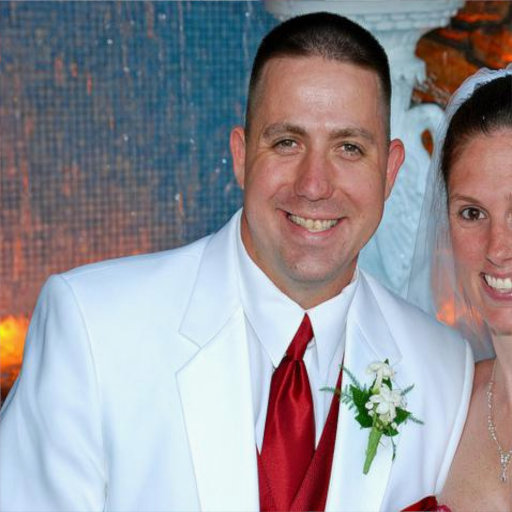
\includegraphics[width=0.15\textwidth]{ch-tomnet/images/Dataset/render_gt_shape003_COCO_val2014_000000366529_ref}
     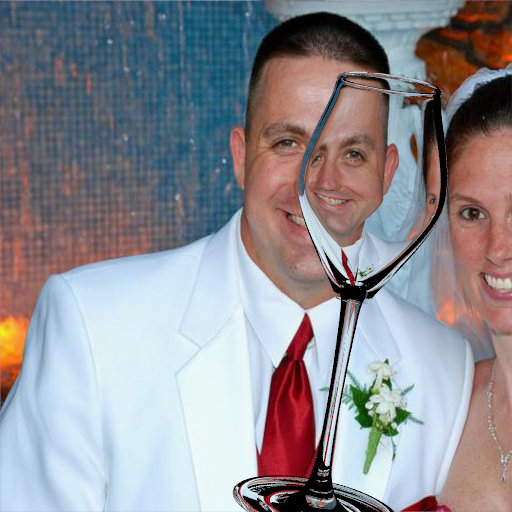
\includegraphics[width=0.15\textwidth]{ch-tomnet/images/Dataset/render_gt_shape003_COCO_val2014_000000366529}
     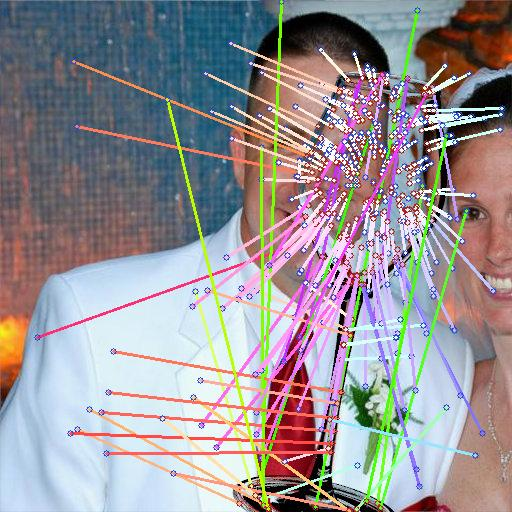
\includegraphics[width=0.15\textwidth]{ch-tomnet/images/Dataset/render_gt_shape003_COCO_val2014_000000366529_cores}
     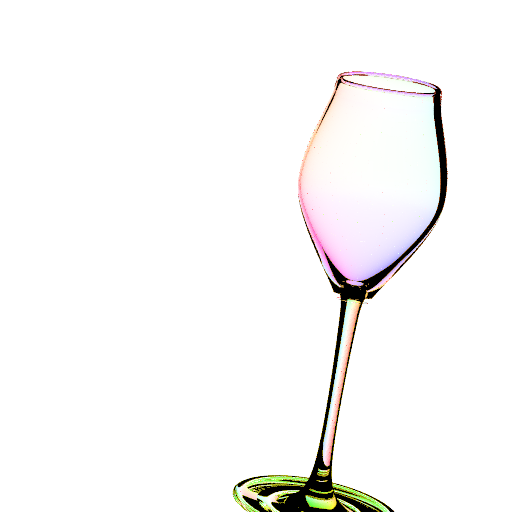
\includegraphics[width=0.15\textwidth]{ch-tomnet/images/Dataset/render_gt_shape003_COCO_val2014_000000366529_flow}
     
\includegraphics[width=0.15\textwidth]{ch-tomnet/images/Dataset/render_gt_shape003_COCO_val2014_000000366529_mask}
     
\includegraphics[width=0.15\textwidth]{ch-tomnet/images/Dataset/render_gt_shape003_COCO_val2014_000000366529_rho}
     \\
     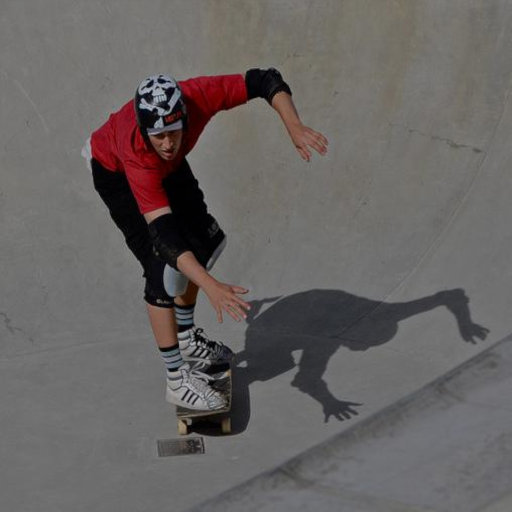
\includegraphics[width=0.15\textwidth]{ch-tomnet/images/Dataset/render_gt_shape002141_0000_COCO_test2015_000000391594_ref}
     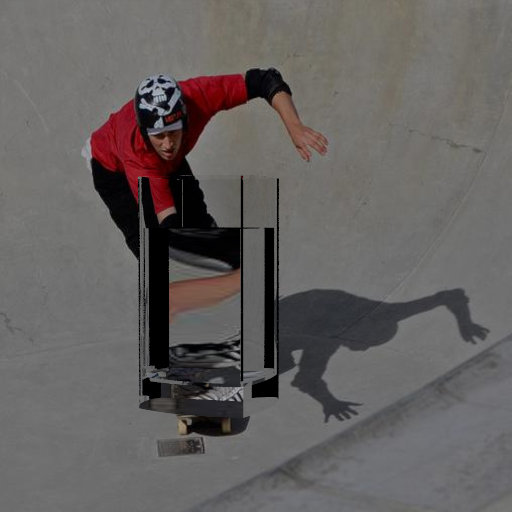
\includegraphics[width=0.15\textwidth]{ch-tomnet/images/Dataset/render_gt_shape002141_0000_COCO_test2015_000000391594}
     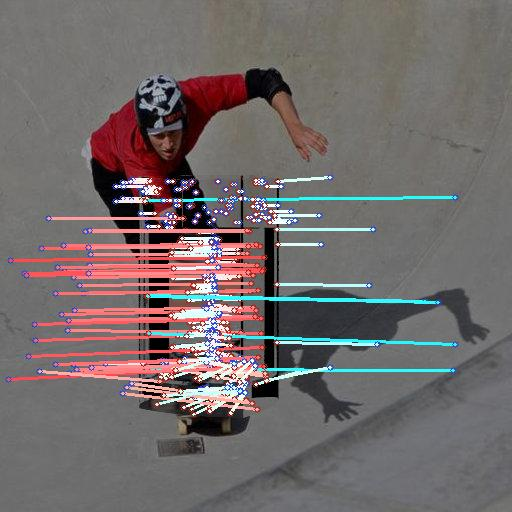
\includegraphics[width=0.15\textwidth]{ch-tomnet/images/Dataset/render_gt_shape0025_000000391594_cores}
     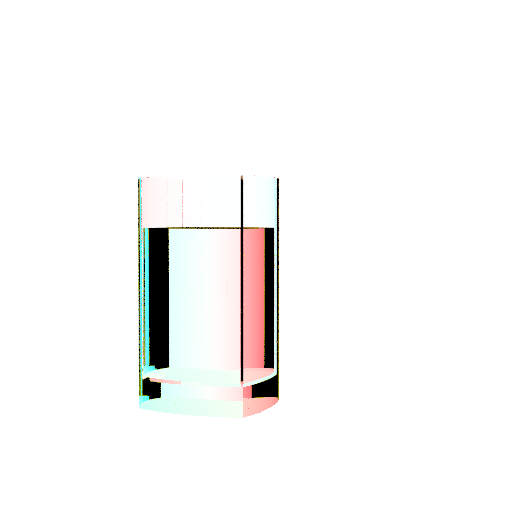
\includegraphics[width=0.15\textwidth]{ch-tomnet/images/Dataset/render_gt_shape0025_000000391594_flow}
     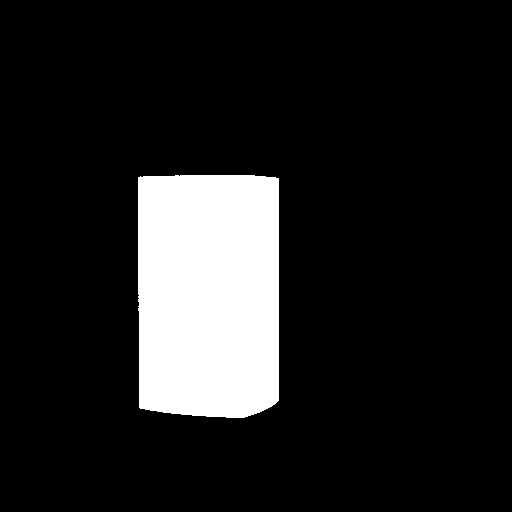
\includegraphics[width=0.15\textwidth]{ch-tomnet/images/Dataset/render_gt_shape0025_000000391594_mask}
     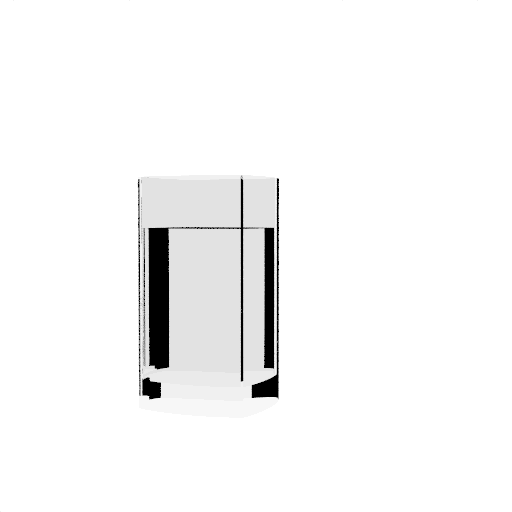
\includegraphics[width=0.15\textwidth]{ch-tomnet/images/Dataset/render_gt_shape002141_0000_COCO_test2015_000000391594_rho}
     \\
     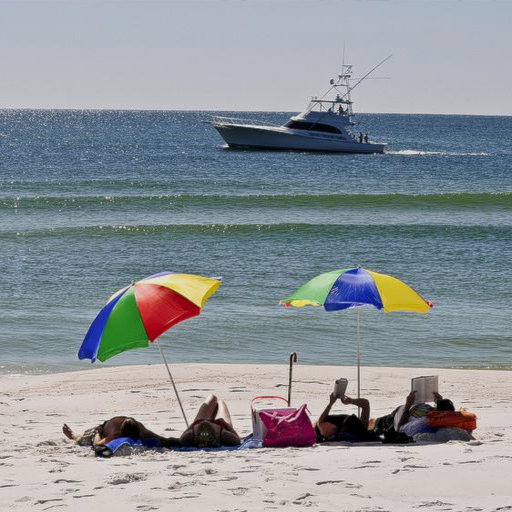
\includegraphics[width=0.15\textwidth]{ch-tomnet/images/Dataset/render_gt_shape0160_COCO_val2014_000000391596_ref}
     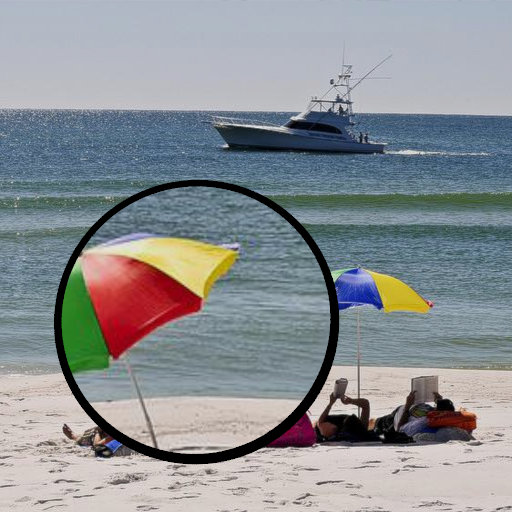
\includegraphics[width=0.15\textwidth]{ch-tomnet/images/Dataset/render_gt_shape0160_COCO_val2014_000000391596}
     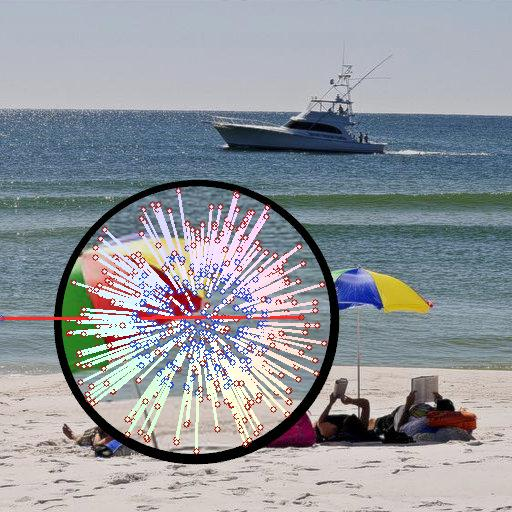
\includegraphics[width=0.15\textwidth]{ch-tomnet/images/Dataset/render_gt_shape0160_COCO_val2014_000000391596_cores}
     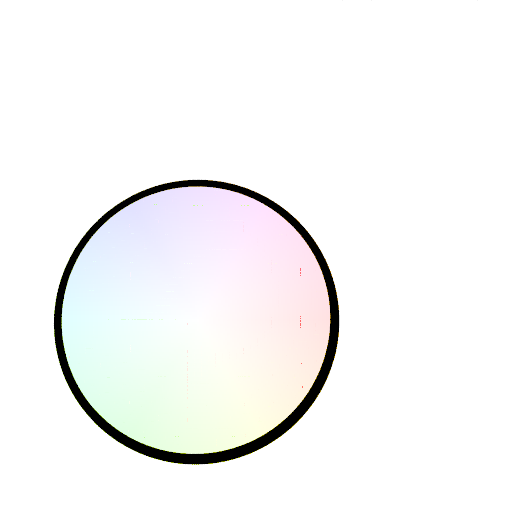
\includegraphics[width=0.15\textwidth]{ch-tomnet/images/Dataset/render_gt_shape0160_COCO_val2014_000000391596_flow}
     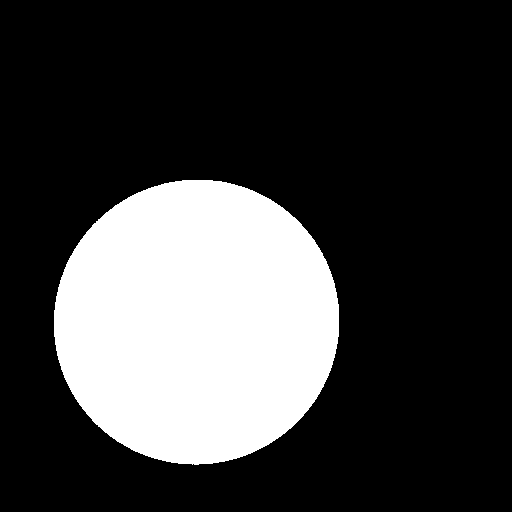
\includegraphics[width=0.15\textwidth]{ch-tomnet/images/Dataset/render_gt_shape0160_COCO_val2014_000000391596_mask}
     
\includegraphics[width=0.15\textwidth]{ch-tomnet/images/Dataset/render_gt_shape0160_COCO_val2014_000000391596_rho}
     \\
     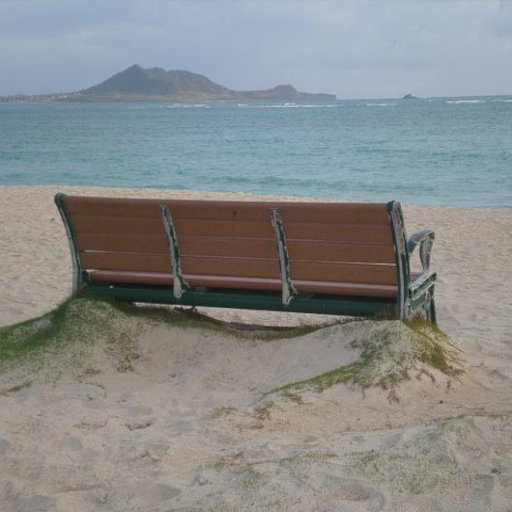
\includegraphics[width=0.15\textwidth]{ch-tomnet/images/Dataset/render_gt_shape0040_COCO_val2014_000000028826_ref}
     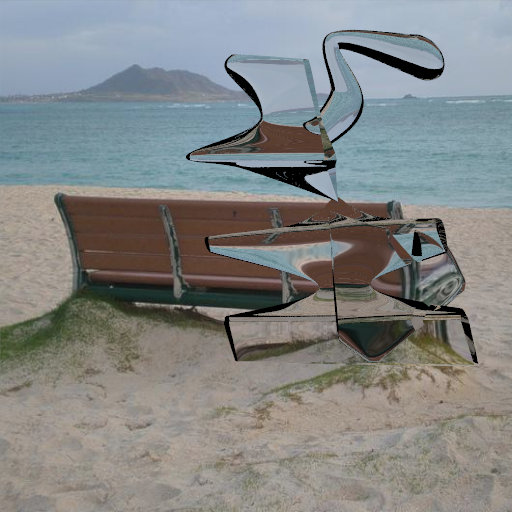
\includegraphics[width=0.15\textwidth]{ch-tomnet/images/Dataset/render_gt_shape0040_COCO_val2014_000000028826}
     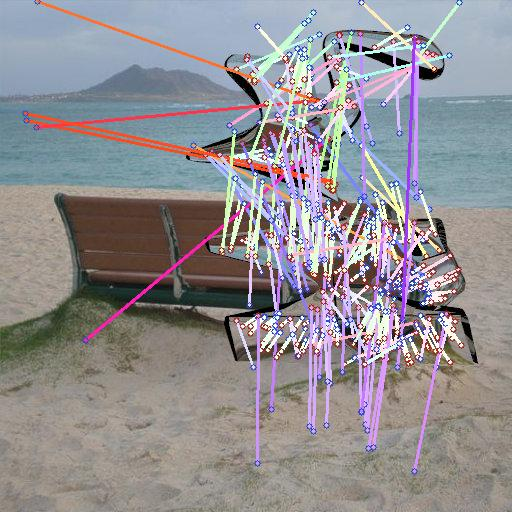
\includegraphics[width=0.15\textwidth]{ch-tomnet/images/Dataset/render_gt_shape0040_COCO_val2014_000000028826_cores}
     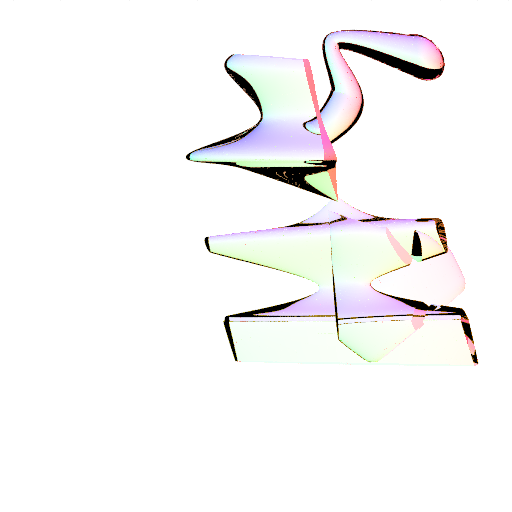
\includegraphics[width=0.15\textwidth]{ch-tomnet/images/Dataset/render_gt_shape0040_COCO_val2014_000000028826_flow}
     
\includegraphics[width=0.15\textwidth]{ch-tomnet/images/Dataset/render_gt_shape0040_COCO_val2014_000000028826_mask}
     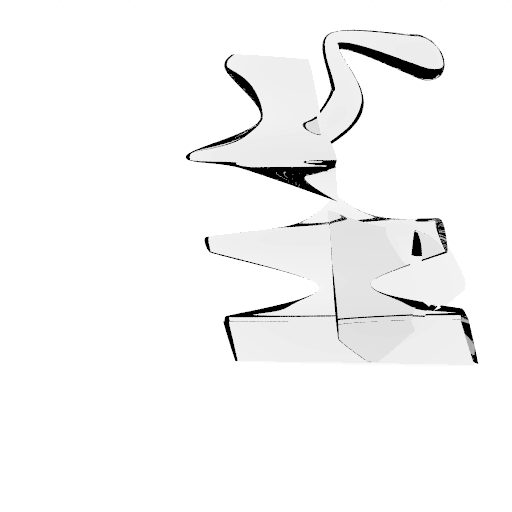
\includegraphics[width=0.15\textwidth]{ch-tomnet/images/Dataset/render_gt_shape0040_COCO_val2014_000000028826_rho}
     \\

    \caption[Examples of synthetic data]{Examples of synthetic data. Top to bottom: examples of \emph{Glass}, \emph{Glass with Water}, \emph{Lens} and \emph{Complex}, respectively. First three columns: background image, rendered image, refractive flow visualization (sparse). Last three columns: ground-truth refractive flow field, object mask, attenuation mask.} 
    \label{fig:syn_data_samples}
\end{figure}

We used a large number of background images and 3D models to render our training samples. We randomly changed the pose of the models, as well as the viewpoint and focal length of the camera in the rendering process to avoid overfitting to a fixed setting.

\paragraph{Background images}
\label{par:Backgrounds Images}
We employed two types of background images, namely scene images and synthetic patterns. For scene images, we randomly sampled images from the Microsoft COCO~\cite{lin2014microsoft} dataset\footnote{Other large-scale datasets like ImageNet~\cite{deng2009imagenet} can also be used.}. The background images for the synthetic training set are sampled from COCO Train2014 and Test2015, while that for the synthetic test dataset are from COCO Val2014, giving rise to $100K$ scene images in total. 
For synthetic patterns, we rendered $40K$ patterns of size $512\times 512$ using \emph{POV-Ray} built-in textures. 

\begin{table} \centering
    \caption[Statistics of our synthetic datasets]{Statistics of our synthetic datasets.}
    \label{tab:synth}
    \resizebox{0.7\textwidth}{!}{
    \Large
    \begin{tabular}{l|*{4}{c}|c}
        \toprule
        Type & \emph{Glass} & \emph{Glass with Water} & \emph{Lens} & \emph{Complex} & Total \\
        \midrule
        Synthetic Train & $52K$ & $26K$ & $20K$ & $80K$ & $178K$\\
        Synthetic Test   & $250$ & $250$ & $200$ & $200$ & $900$\\
        \bottomrule
    \end{tabular}
    }
\end{table}

\paragraph{Transparent objects}
\label{par:Transparent Object}
We divided common transparent objects into four categories, namely \emph{Glass}, \emph{Glass with water}, \emph{Lens}, and \emph{Complex} shape (see \fref{fig:syn_data_samples} for examples). We constructed parametric 3D models for the first three categories, and generated a large number of models using random parameters. For complex shapes, we constructed parametric 3D models for basic shapes like sweeping-spheres and squashed surface of revolution (SOR) parts, and composed a larger number of models using these basic shapes. We generated $178K$ 3D models in total, with each model assigned a random refractive index $\lambda \in [1.3, 1.5]$. The distribution of these models in four categories is shown in \Tref{tab:synth}. 

\paragraph{Ground-truth matte generation}
\label{par:Ground Truth Generation}
We obtained the ground-truth object mask of a model by rendering it in front of a black background image and setting its color to white. Similarly, we obtained the ground-truth attenuation mask of a model by simply rendering it in front of a white background image. Finally, we obtained the ground-truth refractive flow field (see \fref{fig:syn_data_samples}) of a model by rendering it in front of a sequence of Gray-coded patterns. Technical details for the data rendering can be found at \url{https://github.com/guanyingc/TOM-Net_Rendering}.


\paragraph{Data augmentation}
To improve the diversity of the training data and narrow the gap between real and synthetic data, extensive data augmentation was carried out on-the-fly. 
For an image of size $512\times 512$ with color intensity normalized to $[0, 1]$, we randomly performed color (brightness, contrast and saturation) augmentation (in a range of $[-0.2, 0.2]$), image scaling (in a range of $[0.875, 1.05]$), noise perturbation (in a range of $[-0.05, 0.05]$), and horizontal/vertical flipping. Besides, we also blurred the object boundary to make the synthetic data visually more natural. A patch with a size of $448\times 448$ was then randomly cropped from an augmented image and used as input to train CoarseNet. To speed up the training and save memory, a smaller patch with a size of $384\times 384$ was used to train RefineNet after the training of CoarseNet.

\begin{figure}[t] \centering
    \makebox[0.16\textwidth]{\footnotesize \emph{Glass}} 
    \makebox[0.16\textwidth]{\footnotesize \emph{Glass with Water}} 
    \makebox[0.16\textwidth]{\footnotesize \emph{Lens}} 
    \makebox[0.16\textwidth]{\footnotesize \emph{Complex}}
    \makebox[0.16\textwidth]{\footnotesize \emph{Complex}}
    \\
        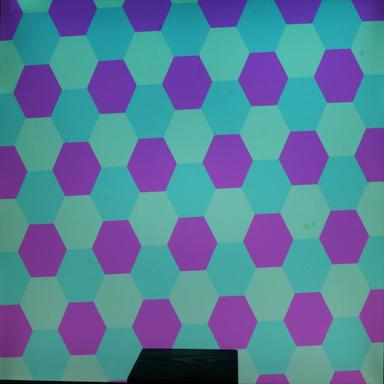
\includegraphics[width=0.16\textwidth]{ch-tomnet/images/Dataset/real_data_Glass_303_bg.jpg}
    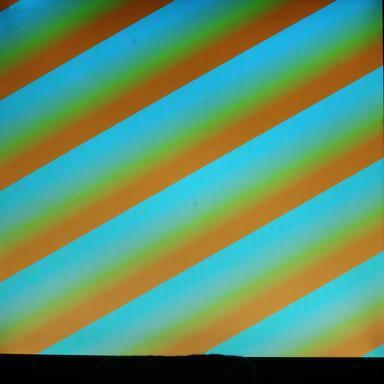
\includegraphics[width=0.16\textwidth]{ch-tomnet/images/Dataset/real_data_Water_064_bg.jpg}
    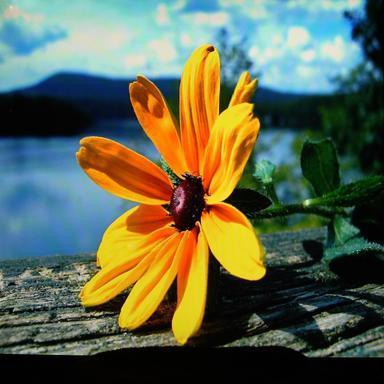
\includegraphics[width=0.16\textwidth]{ch-tomnet/images/Dataset/real_data_Lens_041_bg.jpg}
    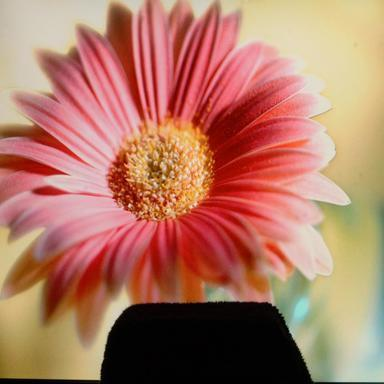
\includegraphics[width=0.16\textwidth]{ch-tomnet/images/Dataset/real_data_Cplx_221_bg.jpg}
    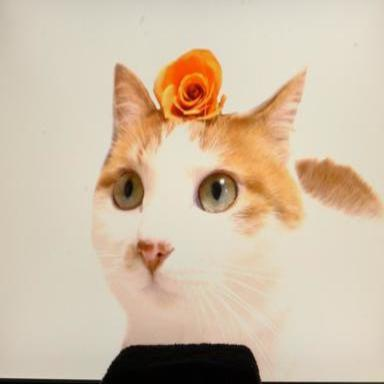
\includegraphics[width=0.16\textwidth]{ch-tomnet/images/Dataset/real_data_Cplx_168_bg.jpg}
    \\
    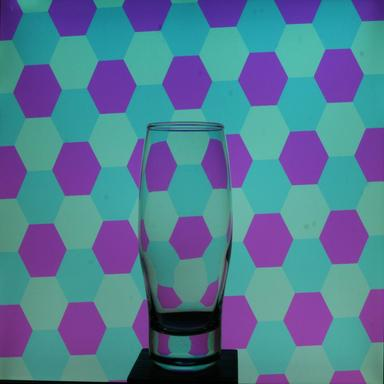
\includegraphics[width=0.16\textwidth]{ch-tomnet/images/Dataset/real_data_Glass_303.jpg}
    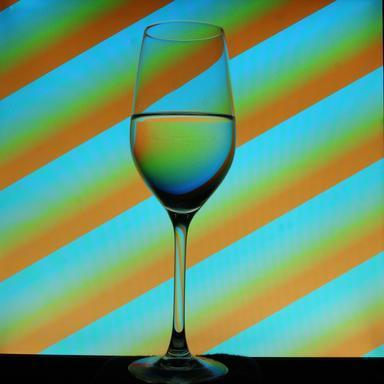
\includegraphics[width=0.16\textwidth]{ch-tomnet/images/Dataset/real_data_Water_064.jpg}
    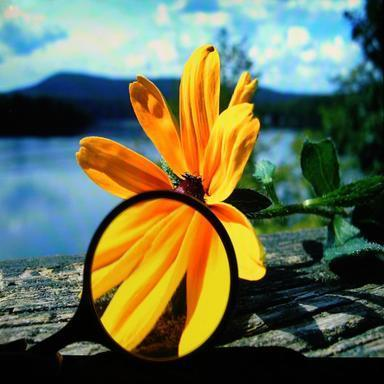
\includegraphics[width=0.16\textwidth]{ch-tomnet/images/Dataset/real_data_Lens_041.jpg}
    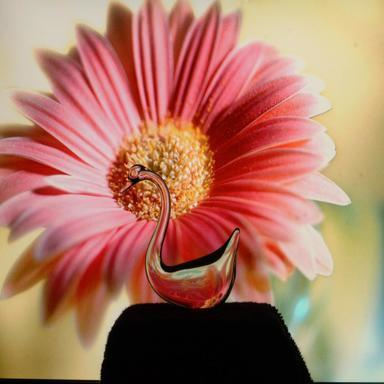
\includegraphics[width=0.16\textwidth]{ch-tomnet/images/Dataset/real_data_Cplx_221.jpg}
    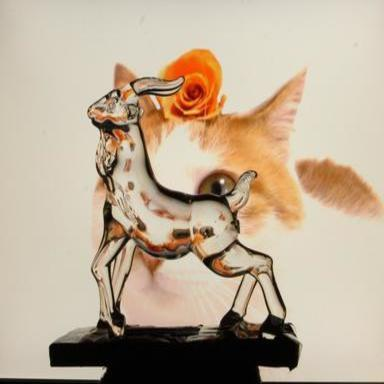
\includegraphics[width=0.16\textwidth]{ch-tomnet/images/Dataset/real_data_Cplx_168.jpg}
    \\

    \caption[Sample images in real dataset]{Sample images in real dataset. The first row shows the background images and the second row shows the images of transparent objects.} \label{fig:real_sample}
\end{figure}

\begin{table}[t] \centering
    \caption[Statistics of our real dataset]{Statistics of our real dataset. The first and second rows show the number of objects and the number of backgrounds used during data acquisition, respectively. The last row shows the number of captured samples. Note that the category of \emph{Glass with Water} are created by filling five of the glasses with different amount of water, and some backgrounds are shared between different shape categories.}
    \label{tab:real_data}
    \resizebox{0.6\textwidth}{!}{
    \Large
    \begin{tabular}{l|*{4}{c}}
        \toprule
        & \emph{Glass} & \emph{Glass with Water} & \emph{Lens} & \emph{Complex} \\% & Total 
        \midrule                                    %
        \# Objects     & $7$   & ($5$ glasses used)  & $1$   & $6$      \\% & 14    
        \# Backgrounds & $60$  & $38$  & $4$   & $18$     \\% & 60    
        \midrule                                    %
        \# Samples     & $470$ & $103$ & $61$  & $242$    \\% & 876   
        \bottomrule
    \end{tabular}
    }
\end{table}
\subsection{Real Dataset}
\label{sub:Real Dataset}
To validate the transferability of TOM-Net, we introduce a real dataset, which was captured using $14$ objects\footnote{The objects consist of $7$ glasses, $1$ lens and $6$ complex objects. Glasses with water are implicitly included.} and $60$ background images, resulting in a dataset of $876$ images. Note that the background images for real data have not been used in the synthetic training or test dataset. The data distribution is summarized in \Tref{tab:real_data}. During the data capturing process, the objects were placed under different poses, with the distances between the camera, object, and background uncontrolled. \fref{fig:real_sample} shows some sample images from the real dataset.  Note that we do not have the ground-truth matte for the real dataset. We instead captured images of the backgrounds without the transparent objects to facilitate evaluation.

Following previous works, the transparent objects were captured in front of a monitor displaying different background images.
Due to the sampling problem, there may exist Moir\'{e}-effect in the captured image.  We carefully adjusted the focal length and shutter speed to remove the Moir\'{e}-effect during the data capturing.

\section{Experimental Results}
\label{sec:experiments}
In this section, we present experimental results and analysis.
We performed ablation study for TOM-Net, and evaluated our approach on both synthetic and real data.  For synthetic data, we evaluated end-point error (EPE) for refractive flow fields, intersection over union (IoU) for object masks, mean square error (MSE) for attenuation masks and image reconstruction results, respectively.  For real data, due to the absence of ground-truth matte, evaluation on the absolute error with respect to the ground truth is not possible. 
Instead, we reconstructed the input images using the estimated mattes and background images, and then evaluated the PSNR and SSIM metrics~\cite{wang2004image} between each pair of input image (\ie, photograph) and reconstructed image (\ie, composite). In addition, a user study was conducted to validate the realism of TOM-Net composites.

We showcased an application of image editing of transparent object by manipulating the extracted matte, and analyzed typical failure cases. We also investigated how the performance of our method can be improved when a trimap or a background image is available.

\subsection{Ablation Study for Network Architecture}
\label{sub:Network Analysis}

\begin{table} \centering
    \caption[Ablation study for TOM-Net]{Ablation study for TOM-Net. F, A, I, and M are short for flow, attenuation, image reconstruction, and object mask, respectively. (The first value for EPE is measured on the whole image and the second measured within the object region. A-MSE and I-MSE are computed on the whole image.)}
    \label{tab:self_compare}
        \resizebox{0.8\textwidth}{!}{
        \begin{tabular}{cl*{4}{c}} %
        \toprule
        ID & Model Variants & \cellcolor{red!25}F-EPE  & \cellcolor{red!25}A-MSE & \cellcolor{red!25}I-MSE &  \cellcolor{blue!25}M-IoU \\ 
        \midrule
        0 & Background                         & 6.5 / 41.0 & 1.58 & 0.87 & 0.15 \\
        1 & CoarseNet - ($\mathL^c_{fr}$) & 3.9 / 26.5 & 0.24 & 0.23 & 0.98 \\
        2 & CoarseNet - (cross-link)           & 2.5 / 17.2 & 0.30 & 0.21 & 0.97  \\
        3 & CoarseNet - (multi-scale)          & 2.4 / 16.6 & 0.69 & 0.25 & 0.94 \\
        4 & CoarseNet - ($\mathL^c_{ir}$) & 2.3 / 15.7 & 0.25 & 0.22 & 0.98 \\
        5 & CoarseNet                          & \textbf{2.2 / 15.4} & 0.28 & 0.18 & 0.97 \\
        \midrule
        6 & CoarseNet + RefineNet              & \textbf{2.0 / 13.7} & 0.25 & 0.19 & 0.97 \\
        7 & CoarseNet + (RefineNet+$\mathL^r_{ir}$) & 2.0 / 13.9 & 0.24 & 0.18 & 0.97 \\
        \bottomrule
    \end{tabular}
    }
    \resizebox{0.17\textwidth}{!}{
        \begin{tabular}{ccc}
            \midrule
            MSE ($\cdot10^{-2}$)  \\
            \cellcolor{red!25} $\downarrow$ better \\
            \cellcolor{blue!25} $\uparrow$ better \\
            \midrule
        \end{tabular}
    }

\end{table}

We quantitatively analyzed different components of TOM-Net using synthetic dataset\footnote{Complex shape is excluded in experiments here to speed up training.}. We first verified the effectiveness of \emph{refractive flow regression loss} ($\mathL^{c}_{fr}$), \emph{cross-link}, \emph{multi-scale loss} and \emph{image reconstruction loss} ($\mathL^{c}_{ir}$) in the coarse stage by removing each of them from \emph{CoarseNet} during training. We then validated the effectiveness of \emph{RefineNet} in recovering details of the refractive flow field.  RefineNet was evaluated by adding it to a trained CoarseNet and was trained while fixing the parameters of CoarseNet. 
For comparison, we also included a naive baseline, denoted as \emph{Background}, by considering a zero matte case (\ie, whole image as object mask, no attenuation, and no refractive flow) where the reconstructed image is the same as the background image. The quantitative results are summarized in \Tref{tab:self_compare} and the qualitative comparisons are shown in \fref{fig:syn_ablation_study}.
Overall, the baseline \emph{Background} was outperformed by all TOM-Net variants with a large margin for all the evaluation metrics, which clearly shows that TOM-Net can successfully learn the matte. 

\paragraph{Effectiveness of refractive flow regression loss} Comparing experiments with IDs 1 \& 5 in \Tref{tab:self_compare}, it can be clearly seen that the CoarseNet trained with the refractive flow regression loss significantly outperformed that without it in refractive flow estimation. This result indicates that image reconstruction loss alone is not enough to supervise the learning of refractive flow. \fref{fig:syn_ablation_study} (a \& e) qualitatively show that the refractive flow regression loss improved the performance of refractive flow estimation.

\begin{figure}[tbp] \centering
        \makebox[0.160\textwidth]{\scriptsize Background} 
    \makebox[0.160\textwidth]{\scriptsize Input} 
    \makebox[0.160\textwidth]{\scriptsize GT Flow} 
    \makebox[0.160\textwidth]{\scriptsize GT Mask} 
    \makebox[0.160\textwidth]{\scriptsize GT Attenuation} 
    \\
    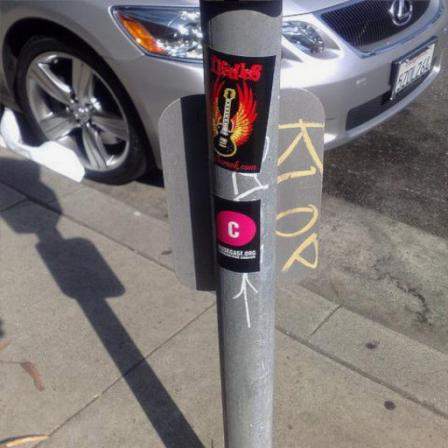
\includegraphics[width=0.160\textwidth]{ch-tomnet/images/Ablation/ablation_290_shape79__0000_COCO_val2014_000000040937_ref.jpg}
    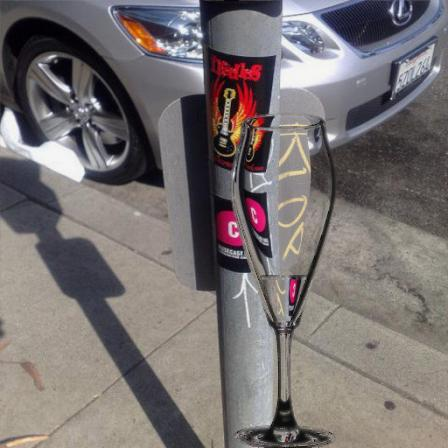
\includegraphics[width=0.160\textwidth]{ch-tomnet/images/Ablation/ablation_290_shape79__0000_COCO_val2014_000000040937_tar.jpg}
    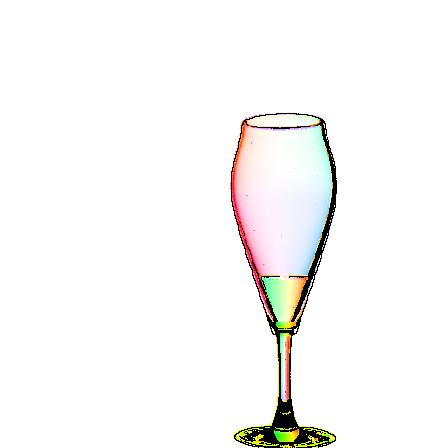
\includegraphics[width=0.160\textwidth]{ch-tomnet/images/Ablation/ablation_290_shape_000000040937_gt_fcolor.jpg}
    
\includegraphics[width=0.160\textwidth]{ch-tomnet/images/Ablation/ablation_290_shape_000000040937_gt_mask}
    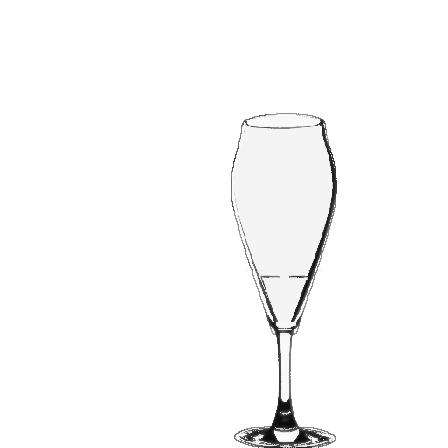
\includegraphics[width=0.160\textwidth]{ch-tomnet/images/Ablation/ablation_290_shape_000000040937_gt_rho.jpg}
    \\ \vspace{-0.4em}\ \hrule\ \\
    \makebox[0.160\textwidth]{\scriptsize (a) \textbf{CNet} - ($\mathcal{L}^c_{fr}$)} 
    \makebox[0.160\textwidth]{\scriptsize (b) \textbf{CNet} - (c-l)} 
    \makebox[0.160\textwidth]{\scriptsize (c) \textbf{CNet} - (m-s)} 
    \makebox[0.160\textwidth]{\scriptsize (d) \textbf{CNet} - ($\mathcal{L}^c_{ir}$)} 
    \makebox[0.160\textwidth]{\scriptsize (e) \textbf{CNet}} 
    \makebox[0.160\textwidth]{\scriptsize (f) \textbf{CNet} + \textbf{RNet}} 
    \\
    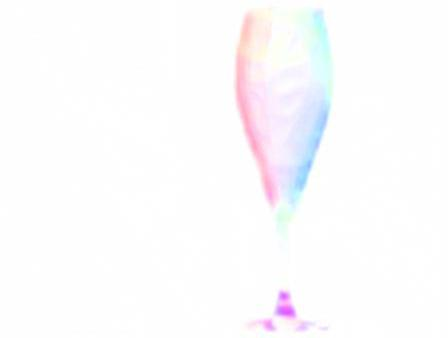
\includegraphics[width=0.160\textwidth]{ch-tomnet/images/Ablation/FlowSup_290_shape0000000040937_fcolor_crop.jpg}
    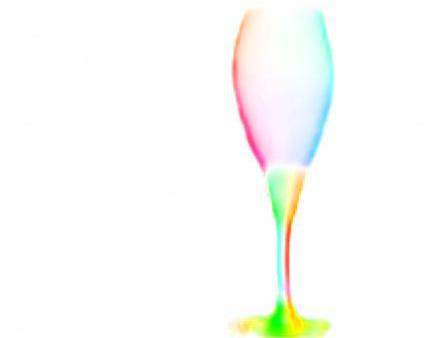
\includegraphics[width=0.160\textwidth]{ch-tomnet/images/Ablation/crosslink_290_shap4_000000040937_fcolor_crop.jpg}
    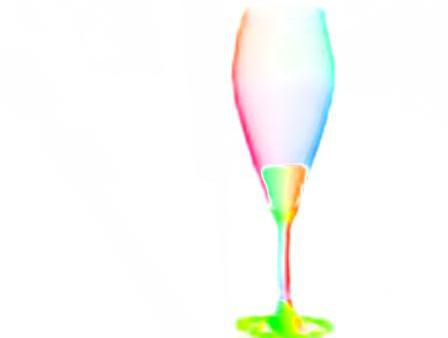
\includegraphics[width=0.160\textwidth]{ch-tomnet/images/Ablation/multiscale_290_sha14_000000040937_fcolor_crop.jpg}
    \includegraphics[width=0.160\textwidth]{ch-tomnet/images/Ablation/recons_290_shape0000000040937_fcolor_crop.jpg}
    \includegraphics[width=0.160\textwidth]{ch-tomnet/images/Ablation/coarse_290_shape0000000040937_fcolor_crop.jpg}
    \includegraphics[width=0.160\textwidth]{ch-tomnet/images/Ablation/ablation_290_shape_000000040937_fcolor_crop.jpg}
    \\
    \makebox[0.160\textwidth]{\tiny \makecell{F-EPE \\ $4.5 / 39.7$}} 
    \makebox[0.160\textwidth]{\tiny \makecell{F-EPE \\ $2.9 / 24.5$}} 
    \makebox[0.160\textwidth]{\tiny \makecell{F-EPE \\ $2.5 / 20.7$}} 
    \makebox[0.160\textwidth]{\tiny \makecell{F-EPE \\ $2.6 / 21.4$}} 
    \makebox[0.160\textwidth]{\tiny \makecell{F-EPE \\ $2.4 / 19.4$}} 
    \makebox[0.160\textwidth]{\tiny \makecell{F-EPE \\ $\mathbf{2.1 / 16.9}$}}
    \\
    \includegraphics[width=0.160\textwidth]{ch-tomnet/images/Ablation/FlowSup_290_shape0000000040937_rho_crop.png}
    \includegraphics[width=0.160\textwidth]{ch-tomnet/images/Ablation/crosslink_290_shap4_000000040937_rho_crop.png}
    \includegraphics[width=0.160\textwidth]{ch-tomnet/images/Ablation/multiscale_290_sha14_000000040937_rho_crop.png}
    \includegraphics[width=0.160\textwidth]{ch-tomnet/images/Ablation/recons_290_shape0000000040937_rho_crop.png}
    \includegraphics[width=0.160\textwidth]{ch-tomnet/images/Ablation/coarse_290_shape0000000040937_rho_crop.png}
    \includegraphics[width=0.160\textwidth]{ch-tomnet/images/Ablation/ablation_290_shape_000000040937_rho_crop.png}
    \\
    \vspace{-0.3em}
    \makebox[0.160\textwidth]{\tiny \makecell{A-MSE \\ $0.19\times 10^{-2}$}}
    \makebox[0.160\textwidth]{\tiny \makecell{A-MSE \\ $0.23\times 10^{-2}$}}
    \makebox[0.160\textwidth]{\tiny \makecell{A-MSE \\ $0.32\times 10^{-2}$}}
    \makebox[0.160\textwidth]{\tiny \makecell{A-MSE \\ $0.21\times 10^{-2}$}}
    \makebox[0.160\textwidth]{\tiny \makecell{A-MSE \\ $0.22\times 10^{-2}$}}
    \makebox[0.160\textwidth]{\tiny \makecell{A-MSE \\ $\mathbf{0.19\times 10^{-2}}$}}
    \\

    \caption[Qualitative comparison of different model variants]{Qualitative comparison of different model variants. The first row shows a sample of \emph{Glass with Water} from the synthetic test dataset. The second and third rows show the estimated refractive flow fields and attenuation masks by different variants, respectively. (\textbf{CNet} and \textbf{RNet} are short for CoarseNet and RefineNet.)} \label{fig:syn_ablation_study}
\end{figure}

\paragraph{Effectiveness of cross-link} Comparing experiments with IDs 2 \& 5 in \Tref{tab:self_compare}, we can see that augmenting the decoders of CoarseNet with cross-link helped improve the performance in all metrics, suggested that utilizing correlation is helpful for the matte estimation.
\fref{fig:syn_ablation_study} (b \& e) qualitatively show the results without and with cross-link during training.

\paragraph{Effectiveness of multi-scale loss} Comparing experiments with IDs 3 \& 5 in \Tref{tab:self_compare}, we can see that multi-scale loss boosted performance of CoarsNet in all of the evaluation metrics, particularly the attenuation mask MSE (see \fref{fig:syn_ablation_study} (c \& e) for qualitative comparison).

\paragraph{Effectiveness of image reconstruction loss} Comparing experiments with IDs 4 \& 5 in \Tref{tab:self_compare}, we can see that adding image reconstruction loss in the coarse stage slightly improved the performance of refractive flow estimation and was very effective for reducing the image reconstruction error (see \fref{fig:syn_ablation_study} (d \& e) for qualitative comparison).

\begin{figure}[tbp] \centering
        \makebox[0.19\textwidth]{\footnotesize Input} 
    \makebox[0.19\textwidth]{\footnotesize Coarse Flow} 
    \makebox[0.19\textwidth]{\footnotesize Refined Flow} 
    \makebox[0.19\textwidth]{\footnotesize Coarse Att.} 
    \makebox[0.19\textwidth]{\footnotesize Refined Att.} 
    \\
    \includegraphics[width=0.19\textwidth]{{ch-tomnet/images/Refine/refine_7_water5_0.90__6_tar}.jpg}
    \includegraphics[width=0.19\textwidth]{{ch-tomnet/images/Refine/refine_7_combine_flow}.jpg}
    \includegraphics[width=0.19\textwidth]{{ch-tomnet/images/Refine/refine_7_combine_r_flow}.jpg}
    \includegraphics[width=0.19\textwidth]{{ch-tomnet/images/Refine/refine_7_combine_rho}.jpg}
    \includegraphics[width=0.19\textwidth]{{ch-tomnet/images/Refine/refine_7_combine_r_rho}.jpg}
    \\
    \includegraphics[width=0.19\textwidth]{{ch-tomnet/images/Refine/refine_5_multi2_1.00__6_tar}.jpg}
    \includegraphics[width=0.19\textwidth]{{ch-tomnet/images/Refine/refine_5_combine_flow}.jpg}
    \includegraphics[width=0.19\textwidth]{{ch-tomnet/images/Refine/refine_5_combine_r_flow}.jpg}
    \includegraphics[width=0.19\textwidth]{{ch-tomnet/images/Refine/refine_5_combine_rho}.jpg}
    \includegraphics[width=0.19\textwidth]{{ch-tomnet/images/Refine/refine_5_combine_r_rho}.jpg}
    \\

    \caption[Visualization of the effectiveness of the refinement stage on real data]{Visualization of the effectiveness of the refinement stage on real data. After refinement, the refractive flow and attenuation mask have more clear structural details (\eg, glass mouth).} \label{fig:refine}
\end{figure}

\paragraph{Effectiveness of RefineNet}
Comparing experiments with IDs 5 \& 6 in \Tref{tab:self_compare}, we can clearly see that RefineNet can significantly improve the refractive flow estimation. \fref{fig:syn_ablation_study} (e \& f) and \fref{fig:refine} show that RefineNet can infer sharp details on both the synthetic and real data based on the outputs of CoarseNet, demonstrating the effectiveness of the RefineNet. We also found that image reconstruction loss is not helpful for refractive flow estimation in the refinement stage (experiments with IDs 6 \& 7 in \Tref{tab:self_compare}). This is reasonable since the matte produced by CoarseNet already gives a small image reconstruction error, and further reducing the image reconstruction error does not guarantee a better refractive flow field. 

\subsection{Evaluation on Synthetic Data}
\label{sub:Results on Synthetic data}
\begin{table*}[htbp] \centering
    \caption[Quantitative results on the synthetic test dataset]{Quantitative results on the synthetic test dataset. (The first value for EPE is measured on the whole image and the second measured within the object region. A-MSE and I-MSE are computed on the whole image.)}
        \resizebox{\textwidth}{!}{
        \Huge
    \begin{tabular}{l*{4}{c}*{4}{c}*{4}{c}*{4}{c}}
        \toprule
            \multirow{2}{*}{} & \multicolumn{4}{c}{\emph{Glass}} 
                               & \multicolumn{4}{c}{\emph{Glass with Water}} 
                               & \multicolumn{4}{c}{\emph{Lens}} 
                               & \multicolumn{4}{c}{\emph{Complex}}  \\
                               & \cellcolor{red!25} F-EPE & \cellcolor{red!25}A-MSE & \cellcolor{red!25}I-MSE & \cellcolor{blue!25} M-IoU 
                               & \cellcolor{red!25} F-EPE & \cellcolor{red!25}A-MSE & \cellcolor{red!25}I-MSE & \cellcolor{blue!25} M-IoU 
                               & \cellcolor{red!25} F-EPE & \cellcolor{red!25}A-MSE & \cellcolor{red!25}I-MSE & \cellcolor{blue!25} M-IoU 
                               & \cellcolor{red!25} F-EPE & \cellcolor{red!25}A-MSE & \cellcolor{red!25}I-MSE & \cellcolor{blue!25} M-IoU \\
        \midrule
        Background    & 3.6 / 30.3 & 1.33 & 0.48 & 0.12 & 6.4 / 53.2 & 1.54 & 0.68 & 0.12 & 10.3 / 39.2 & 1.94 & 1.57 & 0.24 & 6.8 / 56.8 & 2.50 & 0.85 & 0.11 \\
        CoarseNet     & 2.1 / 15.8 & 0.22 & 0.14 & 0.97 & 3.1 / 23.5 & 0.31 & 0.23 & 0.97 & 2.0 / 6.7   & 0.17 & 0.28 & 0.99 & 4.5 / 34.4 & 0.38 & 0.33 & 0.92 \\
        \midrule
        TOM-Net       & 1.9 / 14.7 & 0.21 & 0.14 & 0.97 & 2.9 / 21.8 & 0.30 & 0.22 & 0.97 & 1.9 / 6.6   & 0.15 & 0.29 & 0.99 & 4.1 / 31.5 & 0.37 & 0.32 & 0.92 \\
        \bottomrule
    \end{tabular} 
    }
    \\ \vspace{0.5em}
    \resizebox{0.33\textwidth}{!}{
    \Huge
    \begin{tabular}{l*{4}{c}}
        \toprule
        \multirow{2}{*}{} & \multicolumn{4}{c}{Average}  \\
                          & \cellcolor{red!25} F-EPE & \cellcolor{red!25}A-MSE & \cellcolor{red!25}I-MSE & \cellcolor{blue!25} M-IoU \\
        \midrule
        Background    & 6.8 / 44.9 & 1.83 & 0.90 & 0.15 \\
        CoarseNet     & 2.9 / 20.1 & 0.27 & 0.24 & \B{0.96} \\
        \midrule
        TOM-Net       & \B{2.7} / \B{18.6} & \B{0.26} & \B{0.24} & \B{0.96} \\
        \bottomrule
    \end{tabular}
    }
    \resizebox{0.11\textwidth}{!}{
    \Huge
    \begin{tabular}{ccc}
        \toprule
        MSE ($\cdot10^{-2}$) \\
        \cellcolor{red!25} $\downarrow$ better  \\ 
        \cellcolor{blue!25} $\uparrow$ better  \\
        \bottomrule
    \end{tabular}
    }

    \label{tab:quant_synth}
\end{table*}

Quantitative results for synthetic test dataset are presented in \Tref{tab:quant_synth}. We compared TOM-Net against \emph{Background} and CoarseNet. Here, to accelerate training convergence, we first trained CoarseNet from scratch using our synthetic dataset excluding the complex shape subset. The trained CoarseNet was then fine-tuned using the entire training set including complex shapes, followed by training of RefineNet on the entire training set with random initialization. Similar to previous experiments, TOM-Net outperformed \emph{Background} by a large margin, and slightly outperformed CoarseNet in both EPE and MSE, which implies more local details can be learned by RefinedNet. 

The average IoU for object mask estimation is $0.96$, indicates that TOM-Net can robustly segment the transparent object given only a single image as input.
Although TOM-Net is not expected to learn highly accurate refractive flow, the average EPE errors ($2.7/18.6$)\footnote{The first value is measured on the whole image and the second measured within the object region.} are very small compared with the size of the input image ($448\times 448$). In this sense, our predicted flow is capable of producing visually plausible refractive effect. The errors of complex shape category are larger than that of others, because complex shapes contain more sharp regions that will induce more errors. 
\Fref{fig:qual_synth} and \Fref{fig:qual_synth2} show the qualitative results on five synthetic objects. The objects in the first four examples come from the test set where each example shows a specific object category. Although the background images and objects in the test set never appear in the training set, TOM-Net can still predict robust matte.
 The last row (\ie, \fref{fig:qual_synth2}~(e)) shows a sample of \emph{complex dog}, which was rendered using a 3D dog model. The pleasing result on the \emph{complex dog} demonstrates that our model can generalize well from simple shapes to complex shapes.

\Fref{fig:qual_synth} shows that the reconstructed images using the estimated mattes (column 2) are very close to the input images (column 2), which empirically verifies that our simplified matting equation \eref{eq:em_simplify3} is sufficiently accurate for this problem.

\begin{figure}[htbp] \centering
        \makebox[0.18\textwidth]{\footnotesize \makecell{Input Image \\ Background}} 
    \makebox[0.18\textwidth]{\footnotesize \makecell{Rec. Image \\ Rec. Error}} 
    \makebox[0.18\textwidth]{\footnotesize \makecell{Refractive Flow \\ GT / Estimation}} 
    \makebox[0.18\textwidth]{\footnotesize \makecell{Object Mask \\ GT / Estimation}}
    \makebox[0.18\textwidth]{\footnotesize \makecell{Attenuation Mask \\ GT / Estimation}}
    \\
    \includegraphics[width=0.18\textwidth]{ch-tomnet/images/Synth/synthetic_179_shap0000_COCO_val2014_000000478055_tar.jpg}
    \includegraphics[width=0.18\textwidth]{ch-tomnet/images/Synth/synthetic_179_shap0000_COCO_val2014_000000478055_pred.jpg}
    \includegraphics[width=0.18\textwidth]{ch-tomnet/images/Synth/synthetic_179_shap000478055_gt_fcolor.jpg}
    \includegraphics[width=0.18\textwidth]{ch-tomnet/images/Synth/synthetic_179_shap0000_COCO_val2014_000000478055_gt_mask}
    \includegraphics[width=0.18\textwidth]{ch-tomnet/images/Synth/synthetic_179_shap0000_COCO_val2014_000000478055_gt_rho}
    \\
    \includegraphics[width=0.18\textwidth]{ch-tomnet/images/Synth/synthetic_179_shap0000_COCO_val2014_000000478055_ref.jpg}
    \includegraphics[width=0.18\textwidth]{ch-tomnet/images/Synth/synthetic_179_shap0000_COCO_val2014_000000478055_diff.jpg}
    \includegraphics[width=0.18\textwidth]{ch-tomnet/images/Synth/synthetic_179_shap0000_COCO_val2014_000000478055_fcolor.jpg}
    \includegraphics[width=0.18\textwidth]{ch-tomnet/images/Synth/synthetic_179_shap0000_COCO_val2014_000000478055_mask.png}
    \includegraphics[width=0.18\textwidth]{ch-tomnet/images/Synth/synthetic_179_shap0000_COCO_val2014_000000478055_rho.png}
    \\
    \makebox[0.18\textwidth]{\footnotesize (a) \emph{Glass}} 
    \makebox[0.18\textwidth]{\footnotesize \makecell{I-MSE \\ $0.21 \times 10^{-2}$}} 
    \makebox[0.18\textwidth]{\footnotesize \makecell{F-EPE \\ 2.6 / 15.0}} 
    \makebox[0.18\textwidth]{\footnotesize \makecell{M-IoU \\ 0.99}}
    \makebox[0.18\textwidth]{\footnotesize \makecell{A-MSE \\ $0.16 \times 10^{-2}$}} 
    \\
    \includegraphics[width=0.18\textwidth]{ch-tomnet/images/Synth/synthetic_63_shape25__0000_COCO_val2014_000000408989_tar.jpg}
    \includegraphics[width=0.18\textwidth]{ch-tomnet/images/Synth/synthetic_63_shape25__0000_COCO_val2014_000000408989_pred.jpg}
    \includegraphics[width=0.18\textwidth]{ch-tomnet/images/Synth/synthetic_63_shape_000000408989_gt_fcolor.jpg}
    \includegraphics[width=0.18\textwidth]{ch-tomnet/images/Synth/synthetic_63_shape_000000408989_gt_mask}
    \includegraphics[width=0.18\textwidth]{ch-tomnet/images/Synth/synthetic_63_shape_000000408989_gt_rho}
    \\
    \includegraphics[width=0.18\textwidth]{ch-tomnet/images/Synth/synthetic_63_shape25__0000_COCO_val2014_000000408989_ref.jpg}
    \includegraphics[width=0.18\textwidth]{ch-tomnet/images/Synth/synthetic_63_shape_000000408989_PSNR_29.23_SSIM_0.941_diff.png}
    \includegraphics[width=0.18\textwidth]{ch-tomnet/images/Synth/synthetic_63_shape_000000408989_fcolor.jpg}
    \includegraphics[width=0.18\textwidth]{ch-tomnet/images/Synth/synthetic_63_shape25__0000_COCO_val2014_000000408989_mask.png}
    \includegraphics[width=0.18\textwidth]{ch-tomnet/images/Synth/synthetic_63_shape25__0000_COCO_val2014_000000408989_rho.png}
    \\
    \makebox[0.18\textwidth]{\footnotesize (b) \emph{Glass with Water}} 
    \makebox[0.18\textwidth]{\footnotesize \makecell{I-MSE \\ $0.15\times 10^{-2}$}}
    \makebox[0.18\textwidth]{\footnotesize \makecell{F-EPE \\ 3.8 / 25.0}}
    \makebox[0.18\textwidth]{\footnotesize \makecell{M-IoU \\ 0.97}}
    \makebox[0.18\textwidth]{\footnotesize \makecell{A-MSE \\ 0.40 $\times 10^{-2}$}}
    \\
    \includegraphics[width=0.18\textwidth]{ch-tomnet/images/Synth/synthetic_15_shape0000_COCO_val2014_000000449828_tar.jpg}
    \includegraphics[width=0.18\textwidth]{ch-tomnet/images/Synth/synthetic_15_shape0000_COCO_val2014_000000449828_pred.jpg}
    \includegraphics[width=0.18\textwidth]{ch-tomnet/images/Synth/synthetic_15_shape000449828_gt_fcolor.jpg}
    \includegraphics[width=0.18\textwidth]{ch-tomnet/images/Synth/synthetic_15_shape0000_COCO_val2014_000000449828_gt_mask}
    \includegraphics[width=0.18\textwidth]{ch-tomnet/images/Synth/synthetic_15_shape0000_COCO_val2014_000000449828_gt_rho}
    \\
    \includegraphics[width=0.18\textwidth]{ch-tomnet/images/Synth/synthetic_15_shape0000_COCO_val2014_000000449828_ref.jpg}
    \includegraphics[width=0.18\textwidth]{ch-tomnet/images/Synth/synthetic_15_shape000449828_PSNR_31.01_SSIM_0.92_.jpg}
    \includegraphics[width=0.18\textwidth]{ch-tomnet/images/Synth/synthetic_15_shape0000_COCO_val2014_000000449828_fcolor.jpg}
    \includegraphics[width=0.18\textwidth]{ch-tomnet/images/Synth/synthetic_15_shape0000_COCO_val2014_000000449828_mask.png}
    \includegraphics[width=0.18\textwidth]{ch-tomnet/images/Synth/synthetic_15_shape0000_COCO_val2014_000000449828_rho.png}
    \\
    \makebox[0.18\textwidth]{\footnotesize (c) \emph{Lens}}
    \makebox[0.18\textwidth]{\footnotesize \makecell{I-MSE \\ $0.079\times 10^{-2}$}}
    \makebox[0.18\textwidth]{\footnotesize \makecell{F-EPE \\ 1.5 / 3.7}}
    \makebox[0.18\textwidth]{\footnotesize \makecell{M-IoU \\ 1.00}}
    \makebox[0.18\textwidth]{\footnotesize \makecell{A-MSE \\ $0.17\times 10^{-2}$}}
    \\

    \caption[Qualitative results on synthetic data (part $1$)]{Qualitative results on synthetic data (part $1$). For each example, the first column shows the input image and background. The second column shows the reconstructed image and reconstruction error map. The last three columns show the ground truth matte and estimation. Quantitative results are shown below each example. Dark region in GT flow indicates no valid flow.} \label{fig:qual_synth}
\end{figure}

\begin{figure}[htbp] \centering
        \makebox[0.18\textwidth]{\footnotesize \makecell{Input Image \\ Background}} 
    \makebox[0.18\textwidth]{\footnotesize \makecell{Rec. Image \\ Rec. Error}} 
    \makebox[0.18\textwidth]{\footnotesize \makecell{Refractive Flow \\ GT / Estimation}} 
    \makebox[0.18\textwidth]{\footnotesize \makecell{Object Mask \\ GT / Estimation}}
    \makebox[0.18\textwidth]{\footnotesize \makecell{Attenuation Mask \\ GT / Estimation}}
    \\
    \includegraphics[width=0.18\textwidth]{ch-tomnet/images/Synth/synthetic_15_shape0000_COCO_val2014_000000311180_tar.jpg}
    \includegraphics[width=0.18\textwidth]{ch-tomnet/images/Synth/synthetic_15_shape0000_COCO_val2014_000000311180_pred.jpg}
    \includegraphics[width=0.18\textwidth]{ch-tomnet/images/Synth/synthetic_15_shape000311180_gt_fcolor.jpg}
    \includegraphics[width=0.18\textwidth]{ch-tomnet/images/Synth/synthetic_15_shape0000_COCO_val2014_000000311180_gt_mask.jpg}
    \includegraphics[width=0.18\textwidth]{ch-tomnet/images/Synth/synthetic_15_shape0000_COCO_val2014_000000311180_gt_rho.jpg}
    \\
    \includegraphics[width=0.18\textwidth]{ch-tomnet/images/Synth/synthetic_15_shape0000_COCO_val2014_000000311180_ref.jpg}
    \includegraphics[width=0.18\textwidth]{ch-tomnet/images/Synth/synthetic_15_shape0000_COCO_val2014_000000311180_diff.jpg}
    \includegraphics[width=0.18\textwidth]{ch-tomnet/images/Synth/synthetic_15_shape0000_COCO_val2014_000000311180_fcolor.jpg}
    \includegraphics[width=0.18\textwidth]{ch-tomnet/images/Synth/synthetic_15_shape0000_COCO_val2014_000000311180_mask.png}
    \includegraphics[width=0.18\textwidth]{ch-tomnet/images/Synth/synthetic_15_shape0000_COCO_val2014_000000311180_rho.png}
    \\ 
    \makebox[0.18\textwidth]{\footnotesize (d) \emph{Complex}}
    \makebox[0.18\textwidth]{\footnotesize \makecell{I-MSE \\ $0.15 \times 10^{-2}$}}
    \makebox[0.18\textwidth]{\footnotesize \makecell{F-EPE \\ 3.4 / 24.3}}
    \makebox[0.18\textwidth]{\footnotesize \makecell{M-IoU \\ 0.97}}
    \makebox[0.18\textwidth]{\footnotesize \makecell{A-MSE \\ $0.18 \times 10^{-2}$}}
    \\
    \includegraphics[width=0.18\textwidth]{ch-tomnet/images/Synth/synthetic_1_dog__0000_gradient_7152_tar.jpg}
    \includegraphics[width=0.18\textwidth]{ch-tomnet/images/Synth/synthetic_1_dog__0000_gradient_7152_pred.jpg}
    \includegraphics[width=0.18\textwidth]{ch-tomnet/images/Synth/synthetic_1_dog__0000_gradient_7152_gt_fcolor.jpg}
    \includegraphics[width=0.18\textwidth]{ch-tomnet/images/Synth/synthetic_1_dog__0000_gradient_7152_gt_mask}
    \includegraphics[width=0.18\textwidth]{ch-tomnet/images/Synth/synthetic_1_dog__0000_gradient_7152_gt_rho}
    \\
    \includegraphics[width=0.18\textwidth]{ch-tomnet/images/Synth/synthetic_1_dog__0000_gradient_7152_ref.jpg}
    \includegraphics[width=0.18\textwidth]{ch-tomnet/images/Synth/synthetic_1_dog__0000_gradient_7152_diff.jpg}
    \includegraphics[width=0.18\textwidth]{ch-tomnet/images/Synth/synthetic_1_dog__0000_gradient_7152_fcolor.jpg}
    \includegraphics[width=0.18\textwidth]{ch-tomnet/images/Synth/synthetic_1_dog__0000_gradient_7152_mask.png}
    \includegraphics[width=0.18\textwidth]{ch-tomnet/images/Synth/synthetic_1_dog__0000_gradient_7152_rho.png}
    \\
    \makebox[0.18\textwidth]{\footnotesize (e) \emph{Complex Dog}} 
    \makebox[0.18\textwidth]{\footnotesize \makecell{I-MSE \\ $0.28\times 10^{-2}$}}
    \makebox[0.18\textwidth]{\footnotesize \makecell{F-EPE \\ 5.05 / 40.6}}
    \makebox[0.18\textwidth]{\footnotesize \makecell{M-IoU \\ 0.96}}
    \makebox[0.18\textwidth]{\footnotesize \makecell{A-MSE \\ $0.16\times 10^{-2}$}}


    \caption[Qualitative results on synthetic data (part $2$)]{Qualitative results on synthetic data (part $2$). For each example, the first column shows the input image and background. The second column shows the reconstructed image and reconstruction error map. The last three columns show the ground truth matte and estimation. Quantitative results are shown below each example. Dark region in GT flow indicates no valid flow.} \label{fig:qual_synth2}
\end{figure}

\clearpage
\subsection{Evaluation on Real Data}
\label{sub:Results}
\begin{table}[htbp] \centering
    \caption[Quantitative results on real data]{Quantitative results on real data. (Value the higher the better.)}
    \resizebox{0.9\textwidth}{!}{ 
    \huge
    \begin{tabular}{c|*{2}{c}|*{2}{c}|*{2}{c}|*{2}{c}|*{2}{c}}
        \toprule
        \multirow{2}{*}{} & \multicolumn{2}{c}{\emph{Glass}} 
                          & \multicolumn{2}{c}{\emph{Glass with Water}} 
                          & \multicolumn{2}{c}{\emph{Lens}} 
                          & \multicolumn{2}{c}{\emph{Complex}} 
                          & \multicolumn{2}{c}{Avg} \\
        & PSNR & SSIM  & PSNR & SSIM & PSNR & SSIM & PSNR & SSIM & PSNR & SSIM \\
        \midrule
        Background    & 22.05 & 0.894 & 20.75 & 0.886 & 18.60 & 0.860 & 16.85 & 0.816 & 19.56 & 0.864 \\ 
        CoarseNet     & 25.09 & 0.921 & 23.53 & 0.911 & 21.13 & 0.895 & 17.89 & 0.835 & 21.91 & 0.891  \\ 
        TOM-Net        & 25.06 & 0.920 & 23.53 & 0.911 & 20.89 & 0.893 & 17.88 & 0.835 & 21.84 & 0.890 \\ 
        \bottomrule
    \end{tabular}
    }
    \label{tab:real_quant}
\end{table}

We evaluated TOM-Net on our captured real dataset, which consists of $876$ images of real objects. The results are shown in \Tref{tab:real_quant}. The average PSNR and SSIM are above $21.0$ and $0.89$ respectively. The values are a bit lower for complex shapes, due to the opaque base of complex objects as well as the sharp regions of the objects that might induce large errors. After training, TOM-Net generalized well to common real transparent objects (see \fref{fig:real_qualitative}). It is worth to note that during training, each sample contains only one object, while TOM-Net can predict reliable matte for images containing multiple objects (see \fref{fig:real_qualitative} (c)), which indicates the transferability and robustness of TOM-Net.

\begin{figure}[htbp] \centering
        \makebox[0.115\textwidth]{\footnotesize Background} 
    \makebox[0.115\textwidth]{\footnotesize Input} 
    \makebox[0.115\textwidth]{\footnotesize Rec. Image} 
    \makebox[0.115\textwidth]{\footnotesize Rec. Error} 
    \makebox[0.115\textwidth]{\footnotesize Ref. Flow} 
    \makebox[0.115\textwidth]{\footnotesize Obj. Mask} 
    \makebox[0.115\textwidth]{\footnotesize Att. Mask} 
    \makebox[0.115\textwidth]{\footnotesize Composite} 
    \\
    \includegraphics[width=0.115\textwidth]{{ch-tomnet/images/Real/single_still_1_multi_bg_1.00_1.0_0_ref}.jpg}
    \includegraphics[width=0.115\textwidth]{{ch-tomnet/images/Real/single_still_1_multi_bg_1.00_1.0_6_tar}.jpg}
    \includegraphics[width=0.115\textwidth]{{ch-tomnet/images/Real/single_still_1_multi_bg_1.00_1.0_5_final_r}.jpg}
    \includegraphics[width=0.115\textwidth]{{ch-tomnet/images/Real/single_still_1_mulPSNR_27.60_SSIM_0.95_diff}.png}
    \includegraphics[width=0.115\textwidth]{{ch-tomnet/images/Real/single_still_1_multi_bg_1.00_1.0_1_fcolor_r}.jpg}
    \includegraphics[width=0.115\textwidth]{{ch-tomnet/images/Real/single_still_1_multi_bg_1.00_1.0_3_mask_r}.png}
    \includegraphics[width=0.115\textwidth]{{ch-tomnet/images/Real/single_still_1_multi_bg_1.00_1.0_4_rho_r}.png}
    \includegraphics[width=0.115\textwidth]{{ch-tomnet/images/Real/single_still_1_multi_bg_1.00_1.0_7_transfer_34}.jpg}
    \\
    \vspace{-0.3em}\makebox[0.25\textwidth]{\scriptsize (a) \emph{Glass} \hfill}
    \makebox[0.3\textwidth]{\scriptsize PSNR = 27.6, SSIM = 0.95}
    \makebox[0.4\textwidth]{\scriptsize }
    \\
    \includegraphics[width=0.115\textwidth]{{ch-tomnet/images/Real/water_1_water_1.00_1.0_0_ref}.jpg}
    \includegraphics[width=0.115\textwidth]{{ch-tomnet/images/Real/water_1_water_1.00_1.0_6_tar}.jpg}
    \includegraphics[width=0.115\textwidth]{{ch-tomnet/images/Real/water_1_water_1.00_1.0_5_final_r}.jpg}
    \includegraphics[width=0.115\textwidth]{{ch-tomnet/images/Real/water_1_water_1.00_1.0_7_PSNR_27.32_SSIM_0.95_diff}.png}
    \includegraphics[width=0.115\textwidth]{{ch-tomnet/images/Real/water_1_water_1.00_1.0_1_fcolor_r}.jpg}
    \includegraphics[width=0.115\textwidth]{{ch-tomnet/images/Real/water_1_water_1.00_1.0_3_mask_r}.png}
    \includegraphics[width=0.115\textwidth]{{ch-tomnet/images/Real/water_1_water_1.00_1.0_4_rho_r}.png}
    \includegraphics[width=0.115\textwidth]{{ch-tomnet/images/Real/water_1_water_1.00_1.0_7_transfer_7}.jpg}
    \\
    \vspace{-0.3em}\makebox[0.25\textwidth]{\scriptsize (b) \emph{Glass with Water} \hfill}
    \makebox[0.3\textwidth]{\scriptsize PSNR = 27.3, SSIM = 0.95}
    \makebox[0.4\textwidth]{\scriptsize }
    \\
    \includegraphics[width=0.115\textwidth]{{ch-tomnet/images/Real/multi_1_multi1_1.00_1.0_0_ref}.jpg}
    \includegraphics[width=0.115\textwidth]{{ch-tomnet/images/Real/multi_1_multi1_1.00_1.0_6_tar}.jpg}
    \includegraphics[width=0.115\textwidth]{{ch-tomnet/images/Real/multi_1_multi1_1.00_1.0_5_final_r}.jpg}
    \includegraphics[width=0.115\textwidth]{{ch-tomnet/images/Real/multi_1_multi1_1.00_1.0_7_PSNR_25.37_SSIM_0.93_diff}.png}
    \includegraphics[width=0.115\textwidth]{{ch-tomnet/images/Real/multi_1_multi1_1.00_1.0_1_fcolor_r}.jpg}
    \includegraphics[width=0.115\textwidth]{{ch-tomnet/images/Real/multi_1_multi1_1.00_1.0_3_mask_r}.png}
    \includegraphics[width=0.115\textwidth]{{ch-tomnet/images/Real/multi_1_multi1_1.00_1.0_4_rho_r}.png}
    \includegraphics[width=0.115\textwidth]{{ch-tomnet/images/Real/multi_1_multi1_1.00_1.0_7_transfer_0}.jpg}
    \\
    \vspace{-0.3em}\makebox[0.25\textwidth]{\scriptsize (c) \emph{Multi-objects} \hfill}
    \makebox[0.3\textwidth]{\scriptsize PSNR = 25.37, SSIM = 0.93}
    \makebox[0.4\textwidth]{\scriptsize }
    \\
    \includegraphics[width=0.115\textwidth]{{ch-tomnet/images/Real/lens_1_lens_1.00_1.0_0_ref}.jpg}
    \includegraphics[width=0.115\textwidth]{{ch-tomnet/images/Real/lens_1_lens_1.00_1.0_6_tar}.jpg}
    \includegraphics[width=0.115\textwidth]{{ch-tomnet/images/Real/lens_1_lens_1.00_1.0_5_final_r}.jpg}
    \includegraphics[width=0.115\textwidth]{{ch-tomnet/images/Real/lens_1_lens_1.00_1.0_7_PSNR_27.15_SSIM_0.91_diff}.png}
    \includegraphics[width=0.115\textwidth]{{ch-tomnet/images/Real/lens_1_lens_1.00_1.0_1_fcolor_r}.jpg}
    \includegraphics[width=0.115\textwidth]{{ch-tomnet/images/Real/lens_1_lens_1.00_1.0_3_mask_r}.png}
    \includegraphics[width=0.115\textwidth]{{ch-tomnet/images/Real/lens_1_lens_1.00_1.0_4_rho_r}.png}
    \includegraphics[width=0.115\textwidth]{{ch-tomnet/images/Real/lens_1_lens_1.00_1.0_7_transfer_20}.jpg}
    \\
    \vspace{-0.3em}\makebox[0.25\textwidth]{\scriptsize (d) \emph{Lens} \hfill}
    \makebox[0.3\textwidth]{\scriptsize PSNR = 27.15, SSIM = 0.91}
    \makebox[0.4\textwidth]{\scriptsize }
    \\
    \includegraphics[width=0.115\textwidth]{{ch-tomnet/images/Real/cplx_112__1.00_1.0_0_ref}.jpg}
    \includegraphics[width=0.115\textwidth]{{ch-tomnet/images/Real/cplx_112__1.00_1.0_6_tar}.jpg}
    \includegraphics[width=0.115\textwidth]{{ch-tomnet/images/Real/cplx_112__1.00_1.0_5_final_r}.jpg}
    \includegraphics[width=0.115\textwidth]{{ch-tomnet/images/Real/cplx_112__1.00_1.0_7_PSNR_25.09_SSIM_0.94_diff}.png}
    \includegraphics[width=0.115\textwidth]{{ch-tomnet/images/Real/cplx_112__1.00_1.0_1_fcolor_r}.jpg}
    \includegraphics[width=0.115\textwidth]{{ch-tomnet/images/Real/cplx_112__1.00_1.0_3_mask_r}.png}
    \includegraphics[width=0.115\textwidth]{{ch-tomnet/images/Real/cplx_112__1.00_1.0_4_rho_r}.png}
    \includegraphics[width=0.115\textwidth]{{ch-tomnet/images/Real/cplx_112__1.00_1.0}.jpg}
    \\
    \vspace{-0.3em}\makebox[0.25\textwidth]{\scriptsize (e) \emph{Complex Fish} \hfill}
    \makebox[0.3\textwidth]{\scriptsize PSNR=25.09, SSIM=0.94}
    \makebox[0.4\textwidth]{\scriptsize }
    \\
    \includegraphics[width=0.115\textwidth]{{ch-tomnet/images/Real/cplx_1_bull_1.00_1.0_0_ref}.jpg}
    \includegraphics[width=0.115\textwidth]{{ch-tomnet/images/Real/cplx_1_bull_1.00_1.0_6_tar}.jpg}
    \includegraphics[width=0.115\textwidth]{{ch-tomnet/images/Real/cplx_1_bull_1.00_1.0_5_final_r}.jpg}
    \includegraphics[width=0.115\textwidth]{{ch-tomnet/images/Real/cplx_1_bull_1.00_1.0_7_PSNR_20.31_SSIM_0.84_diff}.png}
    \includegraphics[width=0.115\textwidth]{{ch-tomnet/images/Real/cplx_1_bull_1.00_1.0_1_fcolor_r}.jpg}
    \includegraphics[width=0.115\textwidth]{{ch-tomnet/images/Real/cplx_1_bull_1.00_1.0_3_mask_r}.png}
    \includegraphics[width=0.115\textwidth]{{ch-tomnet/images/Real/cplx_1_bull_1.00_1.0_4_rho_r}.png}
    \includegraphics[width=0.115\textwidth]{{ch-tomnet/images/Real/cplx_1_bull_1.00_1.0_7_transfer_33}.jpg}
    \\                                                                          
    \vspace{-0.3em}\makebox[0.25\textwidth]{\scriptsize (f) \emph{Complex Bull} \hfill}
    \makebox[0.3\textwidth]{\scriptsize PSNR = 20.31, SSIM = 0.84}
    \makebox[0.4\textwidth]{\scriptsize }
    \\
    \includegraphics[width=0.115\textwidth]{{ch-tomnet/images/Real/cplx_2_dragon_1.00_1.0_0_ref}.jpg}
    \includegraphics[width=0.115\textwidth]{{ch-tomnet/images/Real/cplx_2_dragon_1.00_1.0_6_tar}.jpg}
    \includegraphics[width=0.115\textwidth]{{ch-tomnet/images/Real/cplx_2_dragon_1.00_1.0_5_final_r}.jpg}
    \includegraphics[width=0.115\textwidth]{{ch-tomnet/images/Real/cplx_2_dragon_1.00_1.0_7_PSNR_18.46_SSIM_0.80_diff}.png}
    \includegraphics[width=0.115\textwidth]{{ch-tomnet/images/Real/cplx_2_dragon_1.00_1.0_1_fcolor_r}.jpg}
    \includegraphics[width=0.115\textwidth]{{ch-tomnet/images/Real/cplx_2_dragon_1.00_1.0_3_mask_r}.png}
    \includegraphics[width=0.115\textwidth]{{ch-tomnet/images/Real/cplx_2_dragon_1.00_1.0_4_rho_r}.png}
    \includegraphics[width=0.115\textwidth]{{ch-tomnet/images/Real/cplx_2_dragon_1.00_1.0_7_transfer_34}.jpg}
    \\
    \vspace{-0.3em}\makebox[0.25\textwidth]{\scriptsize (g) \emph{Complex Dragon} \hfill}
    \makebox[0.3\textwidth]{\scriptsize PSNR = 18.46, SSIM = 0.80}
    \makebox[0.4\textwidth]{\scriptsize }
    \\
    \includegraphics[width=0.115\textwidth]{{ch-tomnet/images/Real/cplx_174__1.00_1.0_0_ref}.jpg}
    \includegraphics[width=0.115\textwidth]{{ch-tomnet/images/Real/cplx_174__1.00_1.0_6_tar}.jpg}
    \includegraphics[width=0.115\textwidth]{{ch-tomnet/images/Real/cplx_174__1.00_1.0_5_final_r}.jpg}
    \includegraphics[width=0.115\textwidth]{{ch-tomnet/images/Real/cplx_174__1.00_1.0_7_PSNR_14.48_SSIM_0.79_diff}.png}
    \includegraphics[width=0.115\textwidth]{{ch-tomnet/images/Real/cplx_174__1.00_1.0_1_fcolor_r}.jpg}
    \includegraphics[width=0.115\textwidth]{{ch-tomnet/images/Real/cplx_174__1.00_1.0_3_mask_r}.png}
    \includegraphics[width=0.115\textwidth]{{ch-tomnet/images/Real/cplx_174__1.00_1.0_4_rho_r}.png}
    \includegraphics[width=0.115\textwidth]{{ch-tomnet/images/Real/cplx_174__1.00_1.0}.jpg}
    \\
    \vspace{-0.3em}\makebox[0.25\textwidth]{\scriptsize (h) \emph{Complex Sheep} \hfill}
    \makebox[0.3\textwidth]{\scriptsize PSNR=14.48, SSIM=0.79}
    \makebox[0.4\textwidth]{\scriptsize }
    \\

    \caption[Qualitative results on real data]{Qualitative results on real data. The PSNR and SSIM between input photographs and reconstructed images are shown below each example. The last column shows the composites on novel backgrounds given the estimated matte.} 
    \label{fig:real_qualitative}
\end{figure}

\paragraph{User study}
\label{par:User Study}
Remember that our goal is to estimate an environment matte that can produce visually realistic refractive effect from the input image, instead of estimating the highly accurate refractive flow.
A user study was carried out to validate the realism of TOM-Net composites. $69$ subjects participated in our user study. At the beginning, we showed each participant photographs of the transparent objects that will be seen during the user study. The objects consisted of $3$ different glasses, $1$ glass with water, $1$ lens, and $1$ complex shape. $40$ samples, including $20$ photographs\footnote{glass $\times$12, glass \& water $\times$4, lens $\times$2, and complex shape $\times$2.} and the corresponding $20$ TOM-Net composites, were then randomly presented to each subject. When showing each sample, we also showed the corresponding background image to the subject for reference. We provided $3$ options for each sample: (P) {\em photograph}, (C) {\em composite}, (N) {\em not distinguishable}.
\Tref{tab:user_study} shows the statistics of the user study. The $69$ participants produced $1,380$ votes for the $20$ real photographs, and $1,380$ votes for the $20$ composites, respectively. The P:C:N ratios are $850:455:75$ and $827:482:71$ for photographs and composites respectively. The per-category ratios also follow a similar trend, indicating close chance of photographs and composites to be considered real, which further demonstrates TOM-Net can produce realistic matte. 

\begin{table}[tbp] \centering
    \caption[User study results]{User study results. P, C, and N are short for votes for photograph, composite, and not distinguishable.}
    \large
    \resizebox{0.8\textwidth}{!}{
        \begin{tabular}{c|*{3}{c}|*{3}{c}|*{3}{c}|*{3}{c}|*{3}{c}}
        \toprule
            \multirow{2}{*}{}  & \multicolumn{3}{c}{\emph{Glass}} 
                               & \multicolumn{3}{c}{\emph{Glass with Water}} 
                               & \multicolumn{3}{c}{\emph{Lens}} 
                               & \multicolumn{3}{c}{\emph{Complex}}  
                               & \multicolumn{3}{c}{All}  \\
                               & P & C & N & P & C & N & P & C & N & P & C & N & P & C & N \\ \midrule
        Photographs        & 522 & 275 & 31 & 163 & 97 & 16 & 74 & 48 & 16 & 91 & 35 & 12 & 850 & 455 & 75 \\
        Composites    & 531 & 266 & 31 & 145 & 113 & 18 & 73 & 52 & 13 & 78 & 51 & 9 & 827 & 482 & 71 \\
        \bottomrule
    \end{tabular}
    }
    \label{tab:user_study}
\end{table}

\begin{figure}[htbp] \centering
    \includegraphics[width=0.8\textwidth]{ch-tomnet/images/user_study/user_study_larger} \\
    \makebox[0.4\textwidth]{\footnotesize Photograph} 
    \makebox[0.4\textwidth]{\footnotesize Composite} 
    \caption[Comparison of the photograph and composite]{Comparison of the photograph and composite. The first row shows the predicted matte, which is estimated by taking the photograph as input to our method. The second row compares the photograph and composite. When looking at the photograph and composite simultaneously, users can easily spot some imperfections of the composites (mostly in the boundary region).}
    \label{fig:sup_user_study}
\end{figure}

Although we stress that TOM-Net can produce visually realistic composites, the results are still less than perfect. When looking at the real image and our composite side-by-side, users can spot some imperfections of the composite (mostly in the boundary region, see \fref{fig:sup_user_study}). Therefore, we did not include such a user study by showing the real image and our composite side-by-side. Otherwise, the result will be biased. In the future, we will strengthen our approach to produce more realistic composites, so that the real image and our composite are indistinguishable even when showing them side-by-side.

\subsection{Transparent Object Editing by Manipulating Environment Matte}
\label{sec:edit_flow}

\begin{figure}[htbp] \centering
    \makebox[0.132\textwidth]{\scriptsize Background} 
    \makebox[0.132\textwidth]{\scriptsize Input} 
    \makebox[0.132\textwidth]{\scriptsize Rec. Image} 
    \makebox[0.132\textwidth]{\scriptsize Rec. Error} 
    \makebox[0.132\textwidth]{\scriptsize Refractive Flow} 
    \makebox[0.132\textwidth]{\scriptsize Object Mask} 
    \makebox[0.132\textwidth]{\scriptsize Attenuation Mask} 
    \\
        \includegraphics[width=0.132\textwidth]{{ch-tomnet/images/Editing/edit_flow_1__1.00_1.0_0_ref}.jpg}
    \includegraphics[width=0.132\textwidth]{{ch-tomnet/images/Editing/edit_flow_1__1.00_1.0_6_tar}.jpg}
    \includegraphics[width=0.132\textwidth]{{ch-tomnet/images/Editing/edit_flow_1__1.00_1.0_5_final_r}.jpg}
    \includegraphics[width=0.132\textwidth]{{ch-tomnet/images/Editing/edit_flow_1__1.00_1.0_7_PSNR_25.69_SSIM_0.95_diff}.png}
    \includegraphics[width=0.132\textwidth]{{ch-tomnet/images/Editing/edit_flow_1__1.00_1.0_1_fcolor_r}.jpg}
    \includegraphics[width=0.132\textwidth]{{ch-tomnet/images/Editing/edit_flow_1__1.00_1.0_3_mask_r}.png}
    \includegraphics[width=0.132\textwidth]{{ch-tomnet/images/Editing/edit_flow_1__1.00_1.0_4_rho_r}.png}


    \makebox[\textwidth]{\footnotesize (a) An example result on \emph{Glass with Water}. Reconstruction error: PSNR=25.69, SSIM=0.95}
    \\
        \raisebox{0.2\height}{\rotatebox{90}{\scriptsize Ref. Flow}}
    \includegraphics[width=0.132\textwidth]{{ch-tomnet/images/Editing/scale_11__1.00_1.0_1_fcolor_r}.jpg}
    \includegraphics[width=0.132\textwidth]{{ch-tomnet/images/Editing/scale_21__1.00_1.0_1_fcolor_r}.jpg}
    \includegraphics[width=0.132\textwidth]{{ch-tomnet/images/Editing/scale_31__1.00_1.0_1_fcolor_r}.jpg}
    \makebox[0.132\textwidth]{}
    \includegraphics[width=0.132\textwidth]{{ch-tomnet/images/Editing/scale_41__1.00_1.0_1_fcolor_r}.jpg}
    \includegraphics[width=0.132\textwidth]{{ch-tomnet/images/Editing/scale_51__1.00_1.0_1_fcolor_r}.jpg}
    \includegraphics[width=0.132\textwidth]{{ch-tomnet/images/Editing/scale_61__1.00_1.0_1_fcolor_r}.jpg} \\
    \vspace{-0.4em}
    \makebox[0.02\textwidth]{} 
    \makebox[0.132\textwidth]{\scriptsize Flow $\times 0.9$}
    \makebox[0.132\textwidth]{\scriptsize Flow $\times 0.8$}
    \makebox[0.132\textwidth]{\scriptsize Flow $\times 0.7$}
    \makebox[0.132\textwidth]{\scriptsize Input}
    \makebox[0.132\textwidth]{\scriptsize Flow $\times 0.6$}
    \makebox[0.132\textwidth]{\scriptsize Flow $\times 0.5$}
    \makebox[0.132\textwidth]{\scriptsize Flow $\times 0.4$}
    \\
    \raisebox{0.2\height}{\rotatebox{90}{\scriptsize Rec. Image}}
    \includegraphics[width=0.132\textwidth]{{ch-tomnet/images/Editing/scale_11__1.00_1.0_5_final_r}.jpg}
    \includegraphics[width=0.132\textwidth]{{ch-tomnet/images/Editing/scale_21__1.00_1.0_5_final_r}.jpg}
    \includegraphics[width=0.132\textwidth]{{ch-tomnet/images/Editing/scale_31__1.00_1.0_5_final_r}.jpg}
    \includegraphics[width=0.132\textwidth]{{ch-tomnet/images/Editing/scale_1__1.00_1.0_6_tar}.jpg}
    \includegraphics[width=0.132\textwidth]{{ch-tomnet/images/Editing/scale_41__1.00_1.0_5_final_r}.jpg}
    \includegraphics[width=0.132\textwidth]{{ch-tomnet/images/Editing/scale_51__1.00_1.0_5_final_r}.jpg}
    \includegraphics[width=0.132\textwidth]{{ch-tomnet/images/Editing/scale_61__1.00_1.0_5_final_r}.jpg} \\
    \vspace{-0.4em}
    \makebox[0.02\textwidth]{\scriptsize }
    \makebox[0.132\textwidth]{\scriptsize 26.06 / 0.95}
    \makebox[0.132\textwidth]{\scriptsize 26.54 / 0.96}
    \makebox[0.132\textwidth]{\scriptsize 27.07 / 0.96}
    \makebox[0.132\textwidth]{\scriptsize }
    \makebox[0.132\textwidth]{\scriptsize \textbf{27.18 / 0.96}}
    \makebox[0.132\textwidth]{\scriptsize 26.70 / 0.96}
    \makebox[0.132\textwidth]{\scriptsize 25.94 / 0.96}
    \\
    \raisebox{0.25\height}{\rotatebox{90}{\scriptsize Rec. Error}}
    \includegraphics[width=0.132\textwidth]{{ch-tomnet/images/Editing/scale_11__1.00_1.0_7_PSNR_26.06_SSIM_0.96_diff}.png}
    \includegraphics[width=0.132\textwidth]{{ch-tomnet/images/Editing/scale_21__1.00_1.0_7_PSNR_26.54_SSIM_0.96_diff}.png}
    \includegraphics[width=0.132\textwidth]{{ch-tomnet/images/Editing/scale_31__1.00_1.0_7_PSNR_27.07_SSIM_0.96_diff}.png}
    \makebox[0.132\textwidth]{}
    \includegraphics[width=0.132\textwidth]{{ch-tomnet/images/Editing/scale_41__1.00_1.0_7_PSNR_27.18_SSIM_0.96_diff}.png}
    \includegraphics[width=0.132\textwidth]{{ch-tomnet/images/Editing/scale_51__1.00_1.0_7_PSNR_26.70_SSIM_0.96_diff}.png}
    \includegraphics[width=0.132\textwidth]{{ch-tomnet/images/Editing/scale_61__1.00_1.0_7_PSNR_25.94_SSIM_0.96_diff}.png}

    \vspace{-0.2em}\makebox[\textwidth]{\footnotesize (b) Rescaling the magnitude of the estimated refractive flow field.}
    \\
    \vspace{0.4em}
        \makebox[0.020\textwidth]{\scriptsize }
    \makebox[0.132\textwidth]{\scriptsize No Editing}
    \makebox[0.132\textwidth]{\scriptsize Translate left}
    \makebox[0.132\textwidth]{\scriptsize Translate right}
    \makebox[0.132\textwidth]{\scriptsize Rotate 40$\degree$}
    \makebox[0.132\textwidth]{\scriptsize Rotate -40$\degree$}
    \makebox[0.132\textwidth]{\scriptsize Rescale $\times 0.78$}
    \makebox[0.132\textwidth]{\scriptsize Rescale $\times 1.35$}
    \\
    \raisebox{0.3\height}{\rotatebox{90}{\scriptsize Composite}}
    \includegraphics[width=0.132\textwidth]{{ch-tomnet/images/Editing/scaleMatte_41__1.00_1.0_5_final_r}.jpg}
    \includegraphics[width=0.132\textwidth]{{ch-tomnet/images/Editing/trans_11__1.00_1.0_5_final_r}.jpg}
    \includegraphics[width=0.132\textwidth]{{ch-tomnet/images/Editing/trans_61__1.00_1.0_5_final_r}.jpg} 
    \includegraphics[width=0.132\textwidth]{{ch-tomnet/images/Editing/rot_31__1.00_1.0_5_final_r}.jpg}
    \includegraphics[width=0.132\textwidth]{{ch-tomnet/images/Editing/rot_51__1.00_1.0_5_final_r}.jpg}
    \includegraphics[width=0.132\textwidth]{{ch-tomnet/images/Editing/scaleMatte_21__1.00_1.0_5_final_r}.jpg}
    \includegraphics[width=0.132\textwidth]{{ch-tomnet/images/Editing/scaleMatte_51__1.00_1.0_5_final_r}.jpg}
 
    \makebox[\textwidth]{\footnotesize (c) Translate, rotate or rescale the environment matte.}
    \caption[Image editing by manipulating the predicted environment matte]{Various novel composites of a \emph{Glass with Water} shape obtained by manipulating the predicted environment matte.} \label{fig:sup_edit}
\end{figure}

Given a single image as input, our TOM-Net can estimate the environment matte as a triplet (consisting of an object mask, an attenuation mask, and a refractive flow field) in a fast feed-forward pass (see \fref{fig:sup_edit} (a) for an example).
Note that the goal of the proposed TOM-Net is to extract an environment matte that can produce realistic refractive effect from a single image, instead of estimating a highly accurate environment matte. 
The reconstructed image in \fref{fig:sup_edit} (a) looks realistic but does not have the same refractive effect as the original input, as the refractive effect of the estimated matte seems stronger. 
By decreasing the magnitude of the estimated refractive flow field\footnote{We simply multiply the refractive flow field by a scaling factor ($<1$).}, we can produce a similar refractive effect as the input image (see \fref{fig:sup_edit} (b)). When the scaling factor becomes $0.6$, the reconstructed image achieved the lowest reconstruction error, with an improvement of $1.49$ and $0.01$ in PSNR and SSIM, respectively.
Apart from rescaling the magnitude of the refractive flow field to adjust the refractive effect of the object, more interesting composites can be obtained by translating, rotating and rescaling the environment matte (see \fref{fig:sup_edit} (c)). 

\subsection{Failure Cases}
\label{sec:Failure Cases}

\begin{figure}[htbp] \centering
    \makebox[0.05\textwidth]{\footnotesize } 
    \makebox[0.18\textwidth]{\footnotesize Input} 
    \makebox[0.18\textwidth]{\footnotesize Refractive Flow} 
    \makebox[0.18\textwidth]{\footnotesize Object Mask} 
    \makebox[0.18\textwidth]{\footnotesize Attenuation Mask} \\
        \raisebox{0.09\textwidth}{\makebox[0.05\textwidth]{\footnotesize (a)}}
    \includegraphics[width=0.18\textwidth]{{ch-tomnet/images/Failure/fail_657_Multi_bg_0_MultiBackgrouds_106_IMG_0240_tar}.jpg}
    \includegraphics[width=0.18\textwidth]{{ch-tomnet/images/Failure/fail_657_Multi_bg_0_MultiBackgrouds_106_IMG_0240_fcolor}.jpg}
    \includegraphics[width=0.18\textwidth]{{ch-tomnet/images/Failure/fail_657_Multi_bg_0_MultiBackgrouds_106_IMG_0240_mask}.png}
    \includegraphics[width=0.18\textwidth]{{ch-tomnet/images/Failure/fail_657_Multi_bg_0_MultiBackgrouds_106_IMG_0240_rho}.png}
    \\
    \raisebox{0.09\textwidth}{\makebox[0.05\textwidth]{\footnotesize (b)}}
    \includegraphics[width=0.18\textwidth]{{ch-tomnet/images/Failure/fail_585_Multi_bg_0_MultiBackgrouds_19_IMG_0154_tar}.jpg}
    \includegraphics[width=0.18\textwidth]{{ch-tomnet/images/Failure/fail_585_Multi_bg_0_MultiBackgrouds_19_IMG_0154_fcolor}.jpg}
    \includegraphics[width=0.18\textwidth]{{ch-tomnet/images/Failure/fail_585_Multi_bg_0_MultiBackgrouds_19_IMG_0154_mask}.png}
    \includegraphics[width=0.18\textwidth]{{ch-tomnet/images/Failure/fail_585_Multi_bg_0_MultiBackgrouds_19_IMG_0154_rho}.png}
    \\

    \caption[Failure cases on real data]{Two failure cases on real data. In (a), our model fails to estimate the upper-part of the matte as there is no visual clue to find the object. In (b), the bottom part of the estimated matte is incomplete as the background image is heavily cluttered and the bottom part of the object is very dark.}
    \label{fig:sup_fail}
\end{figure}

Our model can robustly estimate environment matte for different transparent objects in front of different backgrounds, however, when there is no visual clue for the objects or the image is too cluttered to separate the object from the background, our model may fail. \Fref{fig:sup_fail} shows two failure cases of our model on real data. In \fref{fig:sup_fail} (a), our model fails to extract the upper-part of the environment matte for the transparent glass due to the lack of visual clue. 
In \fref{fig:sup_fail} (b), although our model is still able to estimate a reasonable matte, the bottom part of the estimated matte is incomplete due to the very cluttered background. 


\subsection{Improvement with Trimap and Background Image}
\begin{table*}[htbp] \centering
    \caption[Quantitative comparison on the synthetic test dataset]{Quantitative comparison between TOM-Net, \TOMNetTrimap and \TOMNetBg on the synthetic test dataset.}
        \resizebox{\textwidth}{!}{
    \Huge
        \begin{tabular}{l*{4}{c}*{4}{c}*{4}{c}*{4}{c}*{4}{c}}
        \toprule
            \multirow{2}{*}{} & \multicolumn{4}{c}{\emph{Glass}} 
                               & \multicolumn{4}{c}{\emph{Glass with Water}} 
                               & \multicolumn{4}{c}{\emph{Lens}} 
                               & \multicolumn{4}{c}{\emph{Complex}}  \\
                               & \cellcolor{red!25} F-EPE & \cellcolor{red!25}A-MSE & \cellcolor{red!25}I-MSE & \cellcolor{blue!25} M-IoU 
                               & \cellcolor{red!25} F-EPE & \cellcolor{red!25}A-MSE & \cellcolor{red!25}I-MSE & \cellcolor{blue!25} M-IoU 
                               & \cellcolor{red!25} F-EPE & \cellcolor{red!25}A-MSE & \cellcolor{red!25}I-MSE & \cellcolor{blue!25} M-IoU 
                               & \cellcolor{red!25} F-EPE & \cellcolor{red!25}A-MSE & \cellcolor{red!25}I-MSE & \cellcolor{blue!25} M-IoU \\
        \midrule
        Background         & 3.6 / 30.3 & 1.33 & 0.48 & 0.12 & 6.4 / 53.2 & 1.54 & 0.68 & 0.12 & 10.3 / 39.2 & 1.94 & 1.57 & 0.24 & 6.8 / 56.8 & 2.50 & 0.85 & 0.11 \\
        \midrule
             TOM-Net       & 1.9 / 14.7 & 0.21 & 0.14 & 0.97 & 2.9 / 21.8 & 0.30 & 0.22 & 0.97 & 1.9 / 6.6   & 0.15 & 0.29 & 0.99 & 4.1 / 31.5 & 0.37 & 0.32 & 0.92 \\
\TOMNetTrimap & 1.8 / 14.4 & 0.21 & 0.14 & 0.98 & 2.6 / 20.7 & 0.29 & 0.20 & 0.98 & 1.7 / 6.1   & 0.15 & 0.27 & 1.00 & 3.7 / 29.4 & 0.37 & 0.29 & 0.95 \\
\TOMNetBg     & 1.6 / 13.1 & 0.21 & 0.12 & 0.99 & 2.4 / 19.3 & 0.29 & 0.19 & 0.98 & 1.4 / 4.9   & 0.18 & 0.19 & 1.00 & 3.5 / 27.7 & 0.36 & 0.27 & 0.97 \\
        \bottomrule
    \end{tabular}
    }
    \\ \vspace{0.5em}
    \resizebox{0.35\textwidth}{!}{
    \Huge
        \begin{tabular}{l*{4}{c}*{4}{c}*{4}{c}*{4}{c}*{4}{c}}
        \toprule
        \multirow{2}{*}{} & \multicolumn{4}{c}{Average}  \\
                          & \cellcolor{red!25} F-EPE & \cellcolor{red!25}A-MSE & \cellcolor{red!25}I-MSE & \cellcolor{blue!25} M-IoU \\
        \midrule
        Background         & 6.8 / 44.9 & 1.83 & 0.90 & 0.15 \\
        \midrule
             TOM-Net       & 2.7 / 18.6 & \textbf{0.26} & 0.24 & 0.96 \\
\TOMNetTrimap & 2.5 / 17.7 & \textbf{0.26} & 0.23 & \textbf{0.98} \\
\TOMNetBg     & \textbf{2.2 / 16.2} & \textbf{0.26} & \textbf{0.19} & \textbf{0.98}\\
        \bottomrule
    \end{tabular}
    }
    \resizebox{0.11\textwidth}{!}{
    \Huge
    \begin{tabular}{ccc}
        \toprule
        MSE ($\cdot10^{-2}$) \\
        \cellcolor{red!25} $\downarrow$ better  \\ 
        \cellcolor{blue!25} $\uparrow$ better  \\
        \bottomrule
    \end{tabular}
    }

    \label{tab:stereo_quant_synth}
\end{table*}

\begin{table}[htbp] \centering
    \caption[Quantitative comparison on real data]{Quantitative comparison between TOM-Net, \TOMNetTrimap and \TOMNetBg on real data.}
    \resizebox{0.8\textwidth}{!}{ 
    \huge
    \begin{tabular}{l|*{2}{c}|*{2}{c}|*{2}{c}|*{2}{c}|*{2}{c}}
        \toprule
        \multirow{2}{*}{} & \multicolumn{2}{c}{\emph{Glass}} 
                          & \multicolumn{2}{c}{\emph{Glass with Water}} 
                          & \multicolumn{2}{c}{\emph{Lens}} 
                          & \multicolumn{2}{c}{\emph{Complex}} 
                          & \multicolumn{2}{c}{Average} \\
        & PSNR & SSIM  & PSNR & SSIM & PSNR & SSIM & PSNR & SSIM & PSNR & SSIM \\
        \midrule
        Background     & 22.05 & 0.894 & 20.75 & 0.886 & 18.60 & 0.860 & 16.85 & 0.816 & 19.56 & 0.864 \\ 
        TOM-Net        & 25.06 & 0.920 & 23.53 & 0.911 & 20.89 & 0.893 & 17.88 & 0.835 & 21.84 & 0.890 \\ 
        \TOMNetTrimap & 25.48 & 0.924 & 23.77 & 0.914 & 23.98 & 0.913 & 20.88 & 0.868 & 23.53 & 0.905\\ 
\TOMNetBg     & 26.10 & 0.931 & 24.58 & 0.922 & 25.52 & 0.924 & 22.23 & 0.884 &\textbf{24.61} & \textbf{0.915} \\ 
        \bottomrule
    \end{tabular}
    }
    \label{tab:real_quant_stereo}
\end{table}

\begin{figure*} \centering
        \makebox[0.155\textwidth]{\footnotesize Testing Input} 
    \makebox[0.155\textwidth]{\footnotesize Rec. Image} 
    \makebox[0.155\textwidth]{\footnotesize Rec. Error} 
    \makebox[0.02\textwidth]{}
    \makebox[0.155\textwidth]{\footnotesize Refractive Flow} 
    \makebox[0.155\textwidth]{\footnotesize Object Mask} 
    \makebox[0.155\textwidth]{\footnotesize Attenu. Mask} 
    \\ %
    \includegraphics[width=0.155\textwidth]{{ch-tomnet/images/Trimap_Bg/mono_35_run_model_1.00_1.0_7_tar}.jpg}
    \includegraphics[width=0.155\textwidth]{{ch-tomnet/images/Trimap_Bg/mono_35_run_model_1.00_1.0_5_final_r}.jpg}
    \includegraphics[width=0.155\textwidth]{{ch-tomnet/images/Trimap_Bg/mono_35_run_model_1.00_1.0_8_PSNR_19.96_SSIM_0.89_diff}.jpg}
    \raisebox{0.2\height}{\rotatebox{90}{\scriptsize 20.0 / 0.89}}
    \includegraphics[width=0.155\textwidth]{{ch-tomnet/images/Trimap_Bg/mono_35_run_model_1.00_1.0_1_fcolor_r}.jpg}
    \includegraphics[width=0.155\textwidth]{{ch-tomnet/images/Trimap_Bg/mono_35_run_model_1.00_1.0_3_mask_r}.jpg}
    \includegraphics[width=0.155\textwidth]{{ch-tomnet/images/Trimap_Bg/mono_35_run_model_1.00_1.0_4_rho_r}.jpg}
    \\
    \includegraphics[width=0.155\textwidth]{{ch-tomnet/images/Trimap_Bg/trimap_horse_0_IMG_0474__trimap}.png}
    \includegraphics[width=0.155\textwidth]{{ch-tomnet/images/Trimap_Bg/trimap_6_006_horse_0_IMG_0474_5_final_r}.jpg}
    \includegraphics[width=0.155\textwidth]{{ch-tomnet/images/Trimap_Bg/trimap_6_006_horse_0_IMG_0474_8_PSNR_28.58_SSIM_0.94_diff}.jpg}
    \raisebox{0.2\height}{\rotatebox{90}{\scriptsize 28.6 / 0.94}}
    \includegraphics[width=0.155\textwidth]{{ch-tomnet/images/Trimap_Bg/trimap_6_006_horse_0_IMG_0474_1_fcolor_r}.jpg}
    \includegraphics[width=0.155\textwidth]{{ch-tomnet/images/Trimap_Bg/trimap_6_006_horse_0_IMG_0474_3_mask_r}.jpg}
    \includegraphics[width=0.155\textwidth]{{ch-tomnet/images/Trimap_Bg/trimap_6_006_horse_0_IMG_0474_4_rho_r}.jpg}
    \\
    \includegraphics[width=0.155\textwidth]{{ch-tomnet/images/Trimap_Bg/stereo_35_run_model_1.00_1.0_0_ref}.jpg}
    \includegraphics[width=0.155\textwidth]{{ch-tomnet/images/Trimap_Bg/stereo_35_run_model_1.00_1.0_5_final_r}.jpg}
    \includegraphics[width=0.155\textwidth]{{ch-tomnet/images/Trimap_Bg/stereo_35_run_model_1.00_1.0_8_PSNR_29.62_SSIM_0.94_diff}.jpg}
    \raisebox{0.2\height}{\rotatebox{90}{\scriptsize 29.6 / 0.94}}
    \includegraphics[width=0.155\textwidth]{{ch-tomnet/images/Trimap_Bg/stereo_35_run_model_1.00_1.0_1_fcolor_r}.jpg}
    \includegraphics[width=0.155\textwidth]{{ch-tomnet/images/Trimap_Bg/stereo_35_run_model_1.00_1.0_3_mask_r}.jpg}
    \includegraphics[width=0.155\textwidth]{{ch-tomnet/images/Trimap_Bg/stereo_35_run_model_1.00_1.0_4_rho_r}.jpg}
    \\
    \vspace{-0.3em} \makebox[0.155\textwidth]{\footnotesize (a) \emph{Complex Horse}} \vspace{0.2em}
    \\
    \includegraphics[width=0.155\textwidth]{{ch-tomnet/images/Trimap_Bg/mono_214_run_model_1.00_1.0_7_tar}.jpg}
    \includegraphics[width=0.155\textwidth]{{ch-tomnet/images/Trimap_Bg/mono_214_run_model_1.00_1.0_5_final_r}.jpg}
    \includegraphics[width=0.155\textwidth]{{ch-tomnet/images/Trimap_Bg/mono_214_run_model_1.00_1.0_8_PSNR_18.59_SSIM_0.81_diff}.jpg}
    \raisebox{0.2\height}{\rotatebox{90}{\scriptsize 18.6 / 0.81}}
    \includegraphics[width=0.155\textwidth]{{ch-tomnet/images/Trimap_Bg/mono_214_run_model_1.00_1.0_1_fcolor_r}.jpg}
    \includegraphics[width=0.155\textwidth]{{ch-tomnet/images/Trimap_Bg/mono_214_run_model_1.00_1.0_3_mask_r}.jpg}
    \includegraphics[width=0.155\textwidth]{{ch-tomnet/images/Trimap_Bg/mono_214_run_model_1.00_1.0_4_rho_r}.jpg}
    \\ %
    \includegraphics[width=0.155\textwidth]{{ch-tomnet/images/Trimap_Bg/trimap_dragon_0_Dragon_4_IMG_0226__trimap}.png}
    \includegraphics[width=0.155\textwidth]{{ch-tomnet/images/Trimap_Bg/trimap_4_004_dragon_0_Dragon_19_IMG_0242_5_final_r}.jpg}
    \includegraphics[width=0.155\textwidth]{{ch-tomnet/images/Trimap_Bg/trimap_Dragon_19_IMG_0242_8_PSNR_19.67_SSIM_0.81_diff}.jpg}
    \raisebox{0.2\height}{\rotatebox{90}{\scriptsize 20.0 / 0.81}}
    \includegraphics[width=0.155\textwidth]{{ch-tomnet/images/Trimap_Bg/trimap_4_004_dragon_0_Dragon_19_IMG_0242_1_fcolor_r}.jpg}
    \includegraphics[width=0.155\textwidth]{{ch-tomnet/images/Trimap_Bg/trimap_4_004_dragon_0_Dragon_19_IMG_0242_3_mask_r}.jpg}
    \includegraphics[width=0.155\textwidth]{{ch-tomnet/images/Trimap_Bg/trimap_4_004_dragon_0_Dragon_19_IMG_0242_4_rho_r}.jpg}
    \\
    \includegraphics[width=0.155\textwidth]{{ch-tomnet/images/Trimap_Bg/stereo_214_run_model_1.00_1.0_0_ref}.jpg}
    \includegraphics[width=0.155\textwidth]{{ch-tomnet/images/Trimap_Bg/stereo_214_run_model_1.00_1.0_5_final_r}.jpg}
    \includegraphics[width=0.155\textwidth]{{ch-tomnet/images/Trimap_Bg/stereo_214_run_model_1.00_1.0_8_PSNR_20.68_SSIM_0.84_diff}.jpg}
    \raisebox{0.2\height}{\rotatebox{90}{\scriptsize 20.7 / 0.84}}
    \includegraphics[width=0.155\textwidth]{{ch-tomnet/images/Trimap_Bg/stereo_214_run_model_1.00_1.0_1_fcolor_r}.jpg}
    \includegraphics[width=0.155\textwidth]{{ch-tomnet/images/Trimap_Bg/stereo_214_run_model_1.00_1.0_3_mask_r}.jpg}
    \includegraphics[width=0.155\textwidth]{{ch-tomnet/images/Trimap_Bg/stereo_214_run_model_1.00_1.0_4_rho_r}.jpg}
    \\
    \vspace{-0.3em}\makebox[0.155\textwidth]{\footnotesize (b) \emph{Complex Dragon}} %

    \caption[Qualitative comparison on real data]{Qualitative comparison between TOM-Net, \TOMNetTrimap and \TOMNetBg on real data.
    For each testing object, the input to the model is shown on the first column, and the results of TOM-Net (up), \TOMNetTrimap (middle) and \TOMNetBg (bottom) are shown on the rest of the columns. Note that for \TOMNetTrimap and \TOMNetBg, we do not show the input image for simplicity. The PSNR and SSIM between input photographs and reconstructed images are shown right after the error maps.}
    \label{fig:qual_stereo_mono}
\end{figure*}

At test time, the input trimaps for \TOMNetTrimap were generated in the same way adopted in the training (as described in \Sref{ssec:trimap}), except that the foreground regions were obtained by performing erosion operation on the ground-truth object mask with a fixed (rather than a random) kernel size of $10$ pixels for evaluation.
\Tref{tab:stereo_quant_synth} shows the quantitative comparisons between TOM-Net, \TOMNetTrimap and \TOMNetBg on the synthetic test dataset. 
As expected, with the access to the additional information, both \TOMNetTrimap and \TOMNetBg performed better than TOM-Net. Due to the fact that a background image contains more useful information than a trimap, \TOMNetBg achieved the best results.

\Tref{tab:real_quant_stereo} presents the quantitative comparison on real data. Compared with TOM-Net, \TOMNetTrimap and \TOMNetBg achieved an improvement of $1.69$ and $2.77$ in average PSNR and an improvement of $0.015$ and $0.024$ in average SSIM, respectively. 
\fref{fig:qual_stereo_mono} shows the qualitative comparison on real data, where the foreground region of the trimap was marked by the user. It can be seen that with the additional information, \TOMNetTrimap and \TOMNetBg can identify the transparent object from the cluttered background more accurately than TOM-Net and model the opaque base of the transparent object (\fref{fig:qual_stereo_mono} (a)). As a result, the environment matte predicted by \TOMNetTrimap and \TOMNetBg can produce more realistic composites and achieve lower reconstruction errors, clearly demonstrating the effectiveness of our framework in handling cases where a trimap or a background image is available.

\section{Discussion}
\label{sec:discussion}

\begin{figure*}[t] \centering
        \makebox[0.02\textwidth]{\footnotesize } 
    \makebox[0.155\textwidth]{\footnotesize Background} 
    \makebox[0.155\textwidth]{\footnotesize Input} 
    \makebox[0.155\textwidth]{\footnotesize Rec. Image} 
    \makebox[0.155\textwidth]{\footnotesize Refractive Flow} 
    \makebox[0.155\textwidth]{\footnotesize Object Mask} 
    \makebox[0.155\textwidth]{\footnotesize Attenuation Mask} 
    \\ 
    \raisebox{4\height}{\makebox[0.02\textwidth]{\footnotesize (a)}}
    \includegraphics[width=0.155\textwidth]{ch-tomnet/images/Limitation/8_colored_030_ref.jpg}
    \includegraphics[width=0.155\textwidth]{ch-tomnet/images/Limitation/8_colored_030_tar.jpg}
    \includegraphics[width=0.155\textwidth]{ch-tomnet/images/Limitation/8_colored_030_pred.jpg}
    \includegraphics[width=0.155\textwidth]{ch-tomnet/images/Limitation/8_colored_030_fcolor.jpg}
    \includegraphics[width=0.155\textwidth]{ch-tomnet/images/Limitation/8_colored_030_mask.png}
    \includegraphics[width=0.155\textwidth]{ch-tomnet/images/Limitation/8_colored_030_rho.png}
\\
    \raisebox{4\height}{\makebox[0.02\textwidth]{\footnotesize (b)}}
    \includegraphics[width=0.155\textwidth]{ch-tomnet/images/Limitation/natural_23_023_IMG_4999crop_0_ref.jpg}
    \includegraphics[width=0.155\textwidth]{ch-tomnet/images/Limitation/natural_23_023_IMG_4999crop_7_tar.jpg}
    \includegraphics[width=0.155\textwidth]{ch-tomnet/images/Limitation/natural_23_023_IMG_4999crop_5_final_r.jpg}
    \includegraphics[width=0.155\textwidth]{ch-tomnet/images/Limitation/natural_23_023_IMG_4999crop_1_fcolor_r.jpg}
    \includegraphics[width=0.155\textwidth]{ch-tomnet/images/Limitation/natural_23_023_IMG_4999crop_3_mask_r.jpg}
    \includegraphics[width=0.155\textwidth]{ch-tomnet/images/Limitation/natural_23_023_IMG_4999crop_4_rho_r.jpg}
\\
    \raisebox{4\height}{\makebox[0.02\textwidth]{\footnotesize (c)}}
    \includegraphics[width=0.155\textwidth]{ch-tomnet/images/Limitation/natural_23_023_IMG_5052crop_0_ref.jpg}
    \includegraphics[width=0.155\textwidth]{ch-tomnet/images/Limitation/natural_23_023_IMG_5052crop_7_tar.jpg}
    \includegraphics[width=0.155\textwidth]{ch-tomnet/images/Limitation/natural_23_023_IMG_5052crop_5_final_r.jpg}
    \includegraphics[width=0.155\textwidth]{ch-tomnet/images/Limitation/natural_23_023_IMG_5052crop_1_fcolor_r.jpg}
    \includegraphics[width=0.155\textwidth]{ch-tomnet/images/Limitation/natural_23_023_IMG_5052crop_3_mask_r.jpg}
    \includegraphics[width=0.155\textwidth]{ch-tomnet/images/Limitation/natural_23_023_IMG_5052crop_4_rho_r.jpg}
\\
    \raisebox{4\height}{\makebox[0.02\textwidth]{\footnotesize (d)}}
    \includegraphics[width=0.155\textwidth]{ch-tomnet/images/Limitation/natural_29_029_IMG_5058crop_0_ref.jpg}
    \includegraphics[width=0.155\textwidth]{ch-tomnet/images/Limitation/natural_29_029_IMG_5058crop_7_tar.jpg}
    \includegraphics[width=0.155\textwidth]{ch-tomnet/images/Limitation/natural_29_029_IMG_5058crop_5_final_r.jpg}
    \includegraphics[width=0.155\textwidth]{ch-tomnet/images/Limitation/natural_29_029_IMG_5058crop_1_fcolor_r.jpg}
    \includegraphics[width=0.155\textwidth]{ch-tomnet/images/Limitation/natural_29_029_IMG_5058crop_3_mask_r.jpg}
    \includegraphics[width=0.155\textwidth]{ch-tomnet/images/Limitation/natural_29_029_IMG_5058crop_4_rho_r.jpg}
\\
    \raisebox{4\height}{\makebox[0.02\textwidth]{\footnotesize (e)}}
    \includegraphics[width=0.155\textwidth]{ch-tomnet/images/Limitation/natural_57_057_IMG_5084crop_0_ref.jpg}
    \includegraphics[width=0.155\textwidth]{ch-tomnet/images/Limitation/natural_57_057_IMG_5084crop_7_tar.jpg}
    \includegraphics[width=0.155\textwidth]{ch-tomnet/images/Limitation/natural_57_057_IMG_5084crop_5_final_r.jpg}
    \includegraphics[width=0.155\textwidth]{ch-tomnet/images/Limitation/natural_57_057_IMG_5084crop_1_fcolor_r.jpg}
    \includegraphics[width=0.155\textwidth]{ch-tomnet/images/Limitation/natural_57_057_IMG_5084crop_3_mask_r.jpg}
    \includegraphics[width=0.155\textwidth]{ch-tomnet/images/Limitation/natural_57_057_IMG_5084crop_4_rho_r.jpg}
\\

    \caption[Results on colored object and objects under natural illumination]{Qualitative results of TOM-Net on colored transparent object (first row) and objects under natural illuminations (last four rows).}
    \label{fig:limitation}
\end{figure*}

\subsection{Limitations}
Although our method can produce plausible results for transparent object matting, there do exist limitations that require further study.
First, our model assumes objects to be colorless so that the attenuation property of an object can be depicted as a scalar value $\rho$ in our formulation. However, this is not applicable to colored transparent objects, as shown in see \fref{fig:limitation}~(a). 
Although our method can estimate a reasonably good object mask and refractive flow field for the \emph{Glass with Water}, the estimated attenuation mask cannot model the colored effect of the object.

Second, our model assumes a single planar background (following most of the previous works) as the only light source and simplifies the interaction between object and background image to a point-to-point (single) mapping. However, more complicated effects exist in the real world, such as specular highlights, translucency, multi-mapping (\ie, refraction and reflection happen simultaneously at a surface point), and color dispersion (\ie, different color components may have different supporting background regions). 
\fref{fig:limitation}~(b)-(e) show four example results of TOM-Net on transparent objects under different types of natural illuminations. Regardless of the fact that TOM-Net can estimate a plausible object mask and refractive flow field, the composites do not look very realistic. 
This is because our current formulation does not consider the more sophisticated refractive properties of a transparent object under natural illumination like complex interaction with environment light, specular highlight, Fresnel effect, and acoustic shadow.

\subsection{Colored Objects and Specular Highlights}
Here we sketch the potential solutions to colored transparent objects as well as the cases when specular highlights appear on transparent objects. In \Sref{sec:formulation}, we simplified matting equation as \eref{eq:em_simplify3}.
To handle colored objects, the scalar attenuation index $\rho$ should be expanded to a color attenuation 3-vector $R$, in which each value corresponds to an attenuation index for a specific color channel. The matting equation then becomes 
\begin{equation}
    \label{eq:color_2}
    C = (1 - m) B + mR \circ \mathcal{M}(\mathbf{T}, P),
\end{equation}
where $\circ$ represents element-wise multiplication.

Consider a white near point light source, we can simplify the specular highlight effect with a specular highlight component $S$, then the generalized matting equation can be written as
\begin{equation}
    \label{eq:color_2}
    C = (1 - m) B + mR \circ \mathcal{M}(\mathbf{T}, P) + S,
\end{equation}
where $S$ is a 3-vector containing three identical values.
The problem of transparent object matting now becomes simultaneously estimating an object mask, a color attenuation mask, a refractive flow field, and a specular highlight mask from a single image, while more efforts are needed to implement them for practical use and we leave this as our future work.

\subsection{Difficulty in Comparison with Previous Works}
Currently, it is not trivial to have a fair comparison with existing methods. On one hand, applying our method on the data used in the previous methods is difficult. Most of the previous methods require multiple images of the transparent object captured in front of pre-designed patterns, which are not publicly available and lack enough textures for our method to estimate the refractive effect of the transparent object. 
The single image based methods RTCEM~\cite{chuang2000environment} and~\cite{yeung2011matting} have additional requirements. In particular, RTCEM~\cite{chuang2000environment} requires the object to be captured in front of a coded-pattern (also not publicly available), and the background image is needed to segment the foreground object. 
\cite{yeung2011matting} requires human interaction to segment the foreground object and model the object's refractive effect with thin-plate-spline transformation. The data used in~\cite{yeung2011matting} does not follow our assumption that the light comes from a single background image, thus it cannot be directly processed by our method.
On the other hand, there are no public implementations for the previous methods, and even if there were, those methods cannot be applied to our dataset which is created for single image transparent object matting.

Different from the previous methods, our method aims to estimate the foreground mask, attenuation mask, and refractive flow field from a single natural image. Since our code and datasets have been made publicly available, it will ease the comparison for the future work. We believe our work can serve as a baseline and provide meaningful insight for future researches in this area.

\subsection{Generalization to Real Data}
    As it is very difficult and time consuming to create a large scale real dataset for training, we use synthetic data for training and evaluate its performance on real data. 
It is well-known that there is a domain gap between the synthetic and real data, and a model trained on synthetic data may not generalize well to real data.
We hypothesize that the reasons why our method works well on real data are as follows.
Following previous works, the real transparent objects are captured in front of a monitor.
Under our assumption, the captured images and the rendered images are very similar. Moreover, extensive data augmentation is performed to close the gap between the synthetic and real data.

To further improve the generalization ability of our method on real data, we will explore the idea of exploiting real data for self-supervised training or fine-tuning in the future.

\subsection{Design of the Network Architecture}
To better recover the details of the refractive flow field and attenuation mask, we propose a two-stage network architecture for this problem. 
Our results show that RefineNet can effectively improve the results of CoarseNet.
However, our two-stage network requires stepwise training (\ie, we first trained CoarseNet until convergence and then trained RefineNet) which requires longer training time.
An interesting future direction is to develop a more efficient single-stage network that achieves comparable performance as the two-stage network. 

\section{Conclusion}
\label{sec:conclusion}
We have introduced a simple and efficient model for transparent object matting, and proposed a CNN architecture, called TOM-Net, that takes a single image as input and predicts environment matte as an object mask, an attenuation mask, and a refractive flow field in a fast feed-forward pass. We created a large-scale synthetic dataset and a real dataset as a benchmark for learning transparent object matting. We have also shown that TOM-Net can perform better by incorporating a trimap or a background image in the input. Promising results have been achieved on both synthetic and real data, which clearly demonstrate the feasibility and effectiveness of the proposed approach. 

\chapter{Learning Photometric Stereo} 
\label{ch:psfcn}

\section{Introduction}
\begin{figure}[t]
\centering
    \includegraphics[width=\textwidth]{ch-psfcn/images/Intro/Intro.pdf}
    \caption[Learning photometric stereo]{Given an arbitrary number of images and their associated light directions as input, our model estimates a normal map of the object in a fast feed-forward pass.} \label{fig:Intro}
\end{figure}

Given multiple images of a static object captured under different light directions with a fixed camera, the surface normals of the object can be estimated using photometric stereo techniques. 
Early calibrated photometric stereo methods assumed a simplified reflectance model, such as the ideal Lambertian model~\cite{woodham1980ps,silver1980determining} or analytical reflectance models~\cite{tozza2016direct,chung2008efficient,ruiters2009heightfield}. 
However, most of the real-world objects are non-Lambertian, and a specific analytical model is only valid for a small set of materials. A bidirectional reflectance distribution function (BRDF) is a general form for describing the reflectance property of a surface, but it is difficult to directly use a non-parametric form of BRDFs for photometric stereo. 
Hence, it remains an open and challenging problem to develop a computationally efficient photometric stereo method that can handle materials with diverse BRDFs. 

Recently, with the great success of deep learning in various computer vision tasks, deep learning based methods have been introduced to calibrated photometric stereo to handle surfaces with general and unknown isotropic reflectance~\cite{santo2017deep,ikehata2018cnn,Taniai18}. Instead of explicitly modeling complex surface reflectances, they directly learn the mapping from reflectance observations to surface normals given known light directions. 
However, the method in~\cite{santo2017deep} depends on a pre-defined set of light directions during training and testing. The methods in~\cite{santo2017deep,ikehata2018cnn} estimate the surface normals in a pixel-wise manner, making them not possible to account for the local context information of a surface point (\eg, surface smoothness prior).
Taniai and Maehara~\cite{Taniai18} introduced an optimization framework based on deep neural network, but their method suffers from complex scenes and requires a long processing time. 

In this work, we propose a deep fully convolutional network (FCN)~\cite{long2015fully}, called PS-FCN for calibrated photometric stereo.
PS-FCN takes an arbitrary number of images with their associated light directions as input, and predicts a surface normal map of the scene in a fast feed-forward pass (see~\fref{fig:Intro}).
Compared with previous learning based methods, our method does not depend on a pre-defined set of light directions during training and testing, and can handle multiple images in an order-agnostic manner. 
Moreover, convolutional neural network (CNN) can naturally incorporate information of the observations at neighboring pixels for computing feature maps, allowing our method to take advantage of local context information. 

To simulate real-world complex non-Lambertian surfaces for training PS-FCN, we create two synthetic datasets using shapes from the blobby shape dataset~\cite{johnson2011shape} and the sculpture shape dataset~\cite{wiles2017silnet}, and BRDFs from the MERL BRDF dataset~\cite{matusik2003merl}. After training on synthetic data, we show that PS-FCN can generalize well on real datasets, including the \diligent~\cite{shi2019benchmark}, the \gourd~\cite{alldrin2008p}, and the \lightstage~\cite{einarsson2006relighting}. 
Extensive experiments on public real datasets show that PS-FCN outperforms existing approaches in calibrated photometric stereo.

Preliminary results of this chapter were published in~\cite{chen2018ps,chen2020deepps}.
Our code, models, and datasets are available at \url{https://guanyingc.github.io/PS-FCN}. 

\section{Related Work}
\label{sec:psfcn_related_work}
In this section, we briefly review representative non-Lambertian photometric stereo techniques. More comprehensive surveys of photometric stereo algorithms can be found in~\cite{herbort2011introduction,shi2019benchmark}. Non-Lambertian photometric stereo methods can be broadly divided into four categories, namely outlier rejection based methods, sophisticated reflectance model based methods, exemplar based methods, and learning based methods.

Outlier rejection based methods assume non-Lambertian observations to be local and sparse such that they can be treated as outliers. Various outlier rejection methods have been proposed so far. They are based on rank minimization~\cite{wu2010robust}, RANSAC~\cite{mukaigawa2007analysis}, taking median values~\cite{miyazaki2010median}, expectation maximization~\cite{wu2010photometric}, and sparse Bayesian regression~\cite{ikehata2012robust}. These outlier rejection methods generally require lots of input images and have difficulty in handling objects with non-sparse non-Lambertian observations (\eg, materials with broad and soft specular highlights).

Many sophisticated reflectance models have been proposed to approximate the non-Lambertian model, including analytical models like Torrance-Sparrow model~\cite{georghiades2003incorporating}, Ward model~\cite{chung2008efficient}, Cook-Torrance model~\cite{ruiters2009heightfield}, etc.
Instead of rejecting specular observations as outliers, sophisticated reflectance model based methods fit an analytical model to all observations.  These methods require solving complex optimization problems, and can only handle limited classes of materials. Recently, bivariate BRDF representations~\cite{shi2014bi,ikehata2014p} were adopted to approximate isotropic BRDF, and a symmetry-based approach~\cite{holroyd2008photometric} was proposed to handle anisotropic reflectance without explicitly estimating a reflectance model. 

Exemplar based methods usually require the observation of an additional reference object. Using a reference sphere, Hertzmann and Seitz~\cite{hertzmann2005example} subtly transformed the non-Lambertian photometric stereo problem to a point matching problem. Exemplar based methods can deal with objects with spatially-varying BRDFs without knowing the light directions, but the requirement of known shape and material of the reference object(s) limits their applications. As an extension, Hui and Sankaranarayanan~\cite{zhui2015ps} introduced a BRDF dictionary to render virtual spheres without using a real reference object, but at the cost of requiring light calibration and longer processing time.

More recently, a few deep learning based methods have been introduced to calibrated photometric stereo~\cite{santo2017deep,Taniai18,ikehata2018cnn}. Santo~\etal~\cite{santo2017deep} proposed a fully-connected network to learn the mapping from reflectance observations captured under a pre-defined set of light directions to surface normal in a pixel-wise manner. 
Ikehata~\cite{ikehata2018cnn} introduced a fixed shape representation, called observation map, that is invariant to the number and permutation of the images. For each surface point of the object, all its observations are merged into an observation map based on the given light directions, and the observation map is then fed to a CNN to regress a normal vector. 
Li~\etal~\cite{li2019learning} and Zheng~\etal~\cite{zheng2019spline} focused on reducing the number of required images while maintaining similar accuracy under the framework proposed by Ikehata~\cite{ikehata2018cnn}.
Compared with~\cite{santo2017deep,ikehata2018cnn}, our method can take advantage of local context information in predicting the surface normals, which results in a more robust behavior.
Taniai and Maehara~\cite{Taniai18} introduced an unsupervised learning framework that predicts both the surface normals and reflectance images of an object. Their model is ``trained'' at test time for each test object by minimizing the reconstruction loss between the input images and the rendered images, while our model is trained with supervised learning and achieves better performance on complex surfaces.

\section{Image Formulation Model}

Following the conventional practice, we assume an orthographic camera with a linear radiometric response, directional lightings coming from the upper-hemisphere, and the viewing direction is parallel to the $z$-axis pointing towards the origin of world coordinates. Let us further assume that the image coordinates is aligned with the world $x\text{-}y$ coordinates.
Consider a non-Lambertian surface whose appearance is described by a general isotropic BRDF $\rho$. Given a surface point with a unit surface normal vector $\vn \in \mathcal{S}^2$, $\mathcal{S}^2 = \{\vv \in \mathbb{R}^3 : \|\vv\|_2 = 1\}$ illuminated by the $j$-th incoming light with direction $\vl_j \in \mathcal{S}^2$ and intensity $e_j \in \mathbb{R}_+$, the image formation model from a fixed viewpoint can be expressed as
\begin{equation}
    \label{eq:formation}
    m_j = e_j \rho (\vn, \vl_j)~\text{max}(\vn^\top \vl_j, 0) + \epsilon_j,
\end{equation}
where $m$ represents the measured intensity, $\text{max}(:, 0)$ operator expresses for attached shadows, and $\epsilon$ accounts for the global illumination effects (\eg, cast shadows and inter-reflections) and noise.

For a Lambertian surface, the BRDF $\rho$ becomes an unknown constant. Theoretically, with three observations captured under non-coplanar light directions (without shadows), the albedo scaled surface normal can be uniquely determined~\cite{woodham1980ps}. 
However, pure Lambertian surfaces barely exist, and we therefore have to consider a more complex problem of non-Lambertian photometric stereo. 

Based on this model, given the observations of surface points (corresponding to individual pixels) under different (known) incoming lights, our method estimates the surface normals for these surface points. Different from traditional methods which approximate $\rho$ with some sophisticated reflectance models, our method directly learns the mapping from images and lightings to surface normals without explicitly modeling $\rho$.

\section{A Flexible Learning Framework for Photometric Stereo}
In this section, we first introduce our strategy for adapting CNNs to handle a variable number of inputs, and then present a flexible fully convolutional network, called PS-FCN, for learning photometric stereo. 

\subsection{Max-pooling for Multi-feature Fusion}
CNNs have been successfully applied to dense regression problems like depth estimation~\cite{eigen2014depth} and surface normal estimation~\cite{wang2015designing}, where the number of input images is fixed and identical during training and testing. Note that adapting CNNs to handle a variable number of inputs during testing is not straightforward, as convolutional layers require the input to have a fixed number of channels during training and testing. Given a variable number of inputs, a shared-weight feature extractor can be used to extract features from each of the inputs (\eg, siamese networks), but an additional fusion layer is required to aggregate such features into a representation with a fixed number of channels. A convolutional layer is applicable for multi-feature fusion only when the number of inputs is fixed. Unfortunately, this is not practical for photometric stereo where the number of inputs often varies.

One possible way to tackle a variable number of inputs is to arrange the inputs sequentially and adopt a recurrent neural network (RNN) to fuse them. For example,~\cite{choy20163d} introduced a RNN framework to unify single- and multi-image 3D voxel prediction. The memory mechanism of RNN enables it to handle sequential inputs, but at the same time also makes it sensitive to the order of inputs. This order sensitive characteristic is not desirable for photometric stereo as it will restrict the illumination changes to follow a specific pattern, making the model less general.

\begin{figure}[t] \centering
    \includegraphics[width=\textwidth]{ch-psfcn/images/Method/pooling.pdf}
    \caption[Multi-feature fusion with max-pooling and average-pooling]{A toy example for max-pooling and average-pooling mechanisms on multi-feature fusion.} \label{fig:pooling}
\end{figure}

More recently, order-agnostic operations (\eg, pooling layers) have been exploited in CNNs to aggregate multi-image information. Wiles and Zisserman~\cite{wiles2017silnet} used max-pooling to fuse features of silhouettes from different views for novel view synthesis and 3D voxel prediction. Hartmann~\etal~\cite{hartmann2017learned} adopted average-pooling to aggregate features of multiple patches for learning multi-patch similarity. In general, max-pooling operation can extract the most salient information from all the features, while average-pooling can smooth out the salient and non-activated features. \fref{fig:pooling} illustrates how max-pooling and average-pooling operations aggregate two features with a toy example.  

For photometric stereo, we argue that max-pooling is a better choice for aggregating features from multiple inputs. 
Our motivation is that, under a certain light direction, regions with high intensities or specular highlights provide strong clues for surface normal inference (\eg, for a surface point with a sharp specular highlight, its normal is close to the bisector of the viewing and light directions). Max-pooling can naturally aggregate such strong features from images captured under different light directions. Besides, max-pooling can ignore non-activated features during training, making it robust to cast shadow. As will be seen in \Sref{sec:psfcn_exp}, our experimental results do validate our arguments. We observe from experiments that each channel of the feature map fused by max-pooling is highly correlated to the response of the surface to a certain light direction. Strong responses in each channel are found in regions with surface normals having similar directions. The feature map can therefore be interpreted as a decomposition of the images under different light directions (see \fref{fig:res_visual}).

\subsection{Network Architecture}
\label{sub:Network Architecture}

\begin{figure}[t] \centering
    \includegraphics[width=\textwidth]{ch-psfcn/images/Method/network_v2}
    \caption{Network architecture of PS-FCN.} \label{fig:network}
\end{figure}

PS-FCN is a multi-input-single-output (MISO) network consisting of three components, namely a shared-weight \emph{feature extractor}, a \emph{fusion layer}, and a \emph{normal regression sub-network} (see \fref{fig:network}). It can be trained and tested using an arbitrary number of images with their associated light directions as input\footnote{For calibrated photometric stereo, the input images are normalized by light intensities, and each light direction is represented by a unit $3$-vector.}.

For each light direction, we have a $3$-channel input image with the dimensions of $3 \times h \times w$, where $h$ and $w$ are the image height and width, respectively. Concatenating images taken under $q$ different lightings $\{\vl_1, ..., \vl_q\}$, we have the data with the dimensions of $q \times 3 \times h \times w$. In addition, we represent the light vectors $\{\vl_1, ..., \vl_q\}$ as $3$-channel images having the same spatial resolution as the input images, resulting in another $q \times 3 \times h \times w$ data. Putting them together, we finally have $q \times 6 \times h \times w$ dimensional inputs to our model.
We separately feed the image-light pairs to the shared-weight feature extractor to extract a feature map from each of the inputs, and apply a max-pooling operation in the fusion layer to aggregate these feature maps. Finally, the normal regression sub-network takes the fused feature map as input and estimates a normal map of the object.

The shared-weight feature extractor has seven convolutional layers, where the feature map is down-sampled twice and then up-sampled once, resulting in a down-sample factor of two. This design can increase the receptive field and preserve spatial information with a small memory consumption. 
The normal regression sub-network has four convolutional layers and up-samples the fused feature map to the same spatial dimension as the input images. A L2-normalization layer is appended at the end of the normal regression sub-network to produce the normal map.

As PS-FCN is a fully convolutional network, it can be applied to datasets with different image sizes. Thanks to the max-pooling operation in the fusion layer, PS-FCN possesses an order-agnostic property. Besides, PS-FCN can be easily extended to handle uncalibrated photometric stereo, where the light directions are not known, by simply removing the light directions during training.

\paragraph{Loss function}
Training of our PS-FCN is supervised by the estimation error between the predicted and the ground-truth normal maps. We formulate our loss function as the commonly used cosine similarity loss, given by
\begin{align}
    \label{eq:normal}
    \mathcal{L}_{\text{Normal}} = \frac{1}{hw} \sum_{i}^{hw} \left(1 - \vn_i^\top \tilde{\vn}_{i} \right),
\end{align}
where $\vn_{i}$ and $\tilde{\vn}_{i}$ denote the predicted normal and the ground-truth normal, respectively, at pixel $i$.
If the predicted normal has a similar orientation as the ground truth, the dot-product $\vn_{i} \cdot \tilde{\vn}_{i}$ will be close to $1$ and the loss becomes small, and vice versa. Other losses like mean squared error can also be alternatively adopted.

\subsection{Data Normalization for Handling Surfaces with SVBRDFs}
As PS-FCN is a fully-convolutional network that processes the input images in a patch-wise manner and is trained on surfaces with homogeneous BRDF, it may have difficulties in dealing with steep color changes caused by surfaces with spatially-varying BRDFs (SVBRDFs), as shown in~\fref{fig:cat_SVBRDF}~(c).
A straightforward idea to tackle this problem is to train a model on surfaces with SVBRDFs. However, creating a large-scale training dataset for this purpose is not trivial, since modeling surface appearance with realistic SVBRDFs requires manual editing from artists.
Even someone can collect a large-scale dataset of objects with SVBRDFs, the created dataset may not be able to faithfully cover the distribution of real data. 
In this work, we introduce a simple yet effective data normalization strategy to enable PS-FCN to handle surfaces with SVBRDFs robustly. We will show that with the proposed data normalization strategy, our method can generalize well to surfaces with SVBRDFs after training only on surfaces with homogeneous BRDF.

\begin{figure}[tbp] \centering
        \makebox[0.190\textwidth]{\footnotesize (a) Object} 
    \makebox[0.190\textwidth]{\footnotesize (b) GT Normal} 
    \makebox[0.190\textwidth]{\footnotesize (c) PS-FCN} 
    \makebox[0.190\textwidth]{\footnotesize (d) PS-FCN$^{\text{+N}}$}
    \\
    \includegraphics[width=0.190\textwidth]{ch-psfcn/images/Results/DiLiGenT/GT/4.0_catPNG_001.png}
    \includegraphics[width=0.190\textwidth]{ch-psfcn/images/Results/DiLiGenT/GT/catPNGGT_normal.png}
    \includegraphics[width=0.190\textwidth]{ch-psfcn/images/Results/DiLiGenT/PS-FCN/catPNGDiLiGenT_normal.png}
    \includegraphics[width=0.190\textwidth]{ch-psfcn/images/Results/DiLiGenT/SVBRDF/PS-FCN_normalized/catPNGDiLiGenT_normal.png}
    \\
    \vspace{-1.2em}
    \makebox[0.190\textwidth]{} 
    \makebox[0.190\textwidth]{} 
    \makebox[0.190\textwidth]{\footnotesize \hfill (6.67)} 
    \makebox[0.190\textwidth]{\footnotesize \hfill (4.67)} 

    \caption[Comparison between PS-FCN and \PSFCNplusN on \emphobject{Cat} with SVBRDF]{Comparison between PS-FCN and \PSFCNplusN on \emphobject{Cat} with spatially-varying BRDFs. Numbers in parentheses denote mean angular error (MAE) in degree.} \label{fig:cat_SVBRDF}
\end{figure}

\begin{figure}[t] \centering
    \includegraphics[width=0.150\textwidth]{ch-psfcn/images/Method/Cat_Normalized/4.0_004.png}
\includegraphics[width=0.150\textwidth]{ch-psfcn/images/Method/Cat_Normalized/4.0_041.png}
\includegraphics[width=0.150\textwidth]{ch-psfcn/images/Method/Cat_Normalized/4.0_048.png}
\includegraphics[width=0.150\textwidth]{ch-psfcn/images/Method/Cat_Normalized/4.0_089.png}
\includegraphics[width=0.150\textwidth]{ch-psfcn/images/Method/Cat_Normalized/4.0_096.png}
\\
\includegraphics[width=0.150\textwidth]{ch-psfcn/images/Method/Cat_Normalized/4.0_1_2_3.png}
\includegraphics[width=0.150\textwidth]{ch-psfcn/images/Method/Cat_Normalized/4.0_1_2_40.png}
\includegraphics[width=0.150\textwidth]{ch-psfcn/images/Method/Cat_Normalized/4.0_1_2_47.png}
\includegraphics[width=0.150\textwidth]{ch-psfcn/images/Method/Cat_Normalized/4.0_1_2_88.png}
\includegraphics[width=0.150\textwidth]{ch-psfcn/images/Method/Cat_Normalized/4.0_1_2_95.png}
\\
\includegraphics[width=0.150\textwidth]{ch-psfcn/images/Method/Ball_Normalized/4.0_004.png}
\includegraphics[width=0.150\textwidth]{ch-psfcn/images/Method/Ball_Normalized/4.0_041.png}
\includegraphics[width=0.150\textwidth]{ch-psfcn/images/Method/Ball_Normalized/4.0_048.png}
\includegraphics[width=0.150\textwidth]{ch-psfcn/images/Method/Ball_Normalized/4.0_089.png}
\includegraphics[width=0.150\textwidth]{ch-psfcn/images/Method/Ball_Normalized/4.0_096.png}
\\
\includegraphics[width=0.150\textwidth]{ch-psfcn/images/Method/Ball_Normalized/4.0_1_1_3.png}
\includegraphics[width=0.150\textwidth]{ch-psfcn/images/Method/Ball_Normalized/4.0_1_1_40.png}
\includegraphics[width=0.150\textwidth]{ch-psfcn/images/Method/Ball_Normalized/4.0_1_1_47.png}
\includegraphics[width=0.150\textwidth]{ch-psfcn/images/Method/Ball_Normalized/4.0_1_1_88.png}
\includegraphics[width=0.150\textwidth]{ch-psfcn/images/Method/Ball_Normalized/4.0_1_1_95.png}
\\

    \caption[Illustration of the introduced data normalization operation]{Illustration of the introduced data normalization operation on \emphobject{cat} and \emphobject{ball} in the \diligent. The first and third rows show the original images, while the second and last rows show the normalized images. Only $5$ out of $96$ images for each object are shown.} \label{fig:normalization_SVBRDF}
\end{figure}

During training, given $q$ observations of a surface point\footnote{Note that the observations are already normalized by the light intensities.}, we concatenate all the observations and normalize them to a unit length vector by
\begin{align}
    \label{eq:normalize}
    \left(m_1', ..., m_{q}'\right) = \left(\frac{m_1}{\sqrt{m_1^2+...+m_{q}^2}}, ..., \frac{m_{q}}{\sqrt{m_1^2+...+m_{q}^2}}\right),
\end{align}
where $m$ and $m'$ represent the original and normalized observations, respectively (for RGB images, we perform normalization on each channel separately). 
The intuition behind this operation is as follows. Consider a Lambertian model, the BRDF $\rho(\vn, \vl)$ degenerates to a constant albedo $\rho$ and $m = \rho \max(\vn^\top \vl_j, 0)$. 
After the data normalization operation, we have
\begin{align}
    \label{eq:normalize2}
    m_{i}' = \frac{\max(\vn^\top \vl_i, 0)}{\sqrt{\max(\vn^\top \vl_1, 0)^2 + \cdots + \max(\vn^\top \vl_q, 0)^2}}.
\end{align}
\Eref{eq:normalize2} shows that the effect of albedo in Lambertian surfaces can be removed after performing data normalization, as shown in the first example in \fref{fig:normalization_SVBRDF}.

However, the above conclusion is not true for non-Lambertian surfaces, because for regions with specular highlights under some light directions, the observations under other light directions will be suppressed after data normalization (see the example of \emphobject{ball} in \fref{fig:normalization_SVBRDF}).
Nevertheless, we experimentally found that such a normalization strategy works equally well for non-Lambertian surfaces under the PS-FCN framework.
This might be explained by the fact that for a non-Lambertian surface under directional lighting, the low-frequency observations are quite close to Lambertian reflectance~\cite{shi2014bi}.
For observations exhibiting specular highlights under some light directions, the max-pooling operation in the fusion layer can naturally ignore the non-activated features (\ie, features extracted from the suppressed observations) and aggregate the most salient features.  
Note that this normalization strategy has also been adopted in~\cite{sato2007shape,lu2013uncalibrated} to compute the similarity between two pixel intensity profiles of non-Lambertian surfaces, while we use this normalization strategy as a preprocessing for CNNs to handle surfaces with SVBRDFs.  

When the number of input images at test time $t$ is different from that in training $q$, the magnitude of the normalized observations will be different, which leads to decreased performance (\eg, when all observations have the same values, 
we have $m_{\text{train}}' = 1/\sqrt{q}, m'_{\text{test}}=1/\sqrt{t}$). 
We experimentally verified that multiplying the normalized observations with the scalar $\sqrt{t/q}$ at test time solves this problem.
We trained a variant model of PS-FCN, denoted as \PSFCNplusN, using the proposed data normalization strategy.
\Fref{fig:cat_SVBRDF}~(d) shows an example result that \PSFCNplusN performed better than PS-FCN on surfaces with SVBRDFs.

\section{Dataset for Learning and Evaluation}
\label{sec:psfcn_dataset}
The training of PS-FCN requires the ground-truth normal maps of the objects. However, obtaining ground-truth normal maps of real objects is a difficult and time-consuming task. Hence, we create two synthetic datasets for training and one synthetic dataset for testing. The publicly available real photometric stereo datasets are reserved to validate the generalization ability of our model. Experimental results show that our PS-FCN trained on the synthetic datasets generalizes well on the challenging real datasets.

\subsection{Synthetic Data for Training}
We used shapes from two existing 3D datasets, namely the blobby shape dataset~\cite{johnson2011shape} and the sculpture shape dataset~\cite{wiles2017silnet}, to generate our training data using the physically based raytracer Mitsuba~\cite{jakob2010mitsuba}. Following DPSN~\cite{santo2017deep}, we employed the MERL dataset~\cite{matusik2003merl}, which contains 100 different BRDFs of real-world materials, to define a diverse set of surface materials for rendering these shapes. 
Note that our datasets explicitly consider cast shadows during rendering.
For the sake of data loading efficiency, we stored our training data in 8-bit PNG format.

\noindent{\bf Blobby dataset\enspace} We first followed~\cite{santo2017deep} to render our training data using the blobby shape dataset~\cite{johnson2011shape}, which contains 10 blobby shapes with various normal distributions. For each blobby shape, $1,296$ regularly-sampled views (36 azimuth angles $\times$ 36 elevation angles) were used, and for each view, 2 out of 100 BRDFs were randomly selected, leading to 25,920 samples ($10\times 36\times 36\times 2$).
For each sample, we rendered 64 images with a spatial resolution of $128 \times 128$ under light directions randomly sampled from a range of 180\degree $\times$ 180\degree, which is more general than the range (74.6\degree $\times$ 51.4\degree) used in the real data benchmark~\cite{shi2019benchmark}. We randomly split this dataset into $99:1$ for training and validation (see \fref{fig:data_samples}(a)).

\begin{figure} \centering
        \begin{subfigure}[t]{0.47\textwidth}
    \centering
    \makebox[0.225\textwidth]{\small (a) Blobby shape.}\\
    \includegraphics[width=0.235\textwidth]{ch-psfcn/images/Dataset/simple/l_000,-0.28,-0.27,0.92_gm.png}
    \includegraphics[width=0.235\textwidth]{ch-psfcn/images/Dataset/simple/l_002,0.60,0.12,0.79_gm.png}
    \includegraphics[width=0.235\textwidth]{ch-psfcn/images/Dataset/simple/l_006,-0.12,0.05,0.99_gm.png}
    \includegraphics[width=0.235\textwidth]{ch-psfcn/images/Dataset/simple/l_022,-0.21,-0.20,0.96_gm.png}\\
    \includegraphics[width=0.235\textwidth]{ch-psfcn/images/Dataset/simple/blob06_s-0.80_x-250_y-250_normal.png}
    \includegraphics[width=0.235\textwidth]{ch-psfcn/images/Dataset/simple/blob02_s-1.00_x-250_y-250_normal.png}
    \includegraphics[width=0.235\textwidth]{ch-psfcn/images/Dataset/simple/blob08_s-0.80_x-250_y-250_normal.png}
    \includegraphics[width=0.235\textwidth]{ch-psfcn/images/Dataset/simple/blob07_s-0.90_x-250_y-250_normal.png}\\
    \end{subfigure}
    \quad
    \begin{subfigure}[t]{0.47\textwidth}
    \centering
    \makebox[0.225\textwidth]{\small (b) Sculpture shape.}\\
    \includegraphics[width=0.235\textwidth]{ch-psfcn/images/Dataset/complex/l_000,-0.41,0.24,0.88_gm.png}
    \includegraphics[width=0.235\textwidth]{ch-psfcn/images/Dataset/complex/l_001,-0.05,0.02,1.00_gm.png}
    \includegraphics[width=0.235\textwidth]{ch-psfcn/images/Dataset/complex/l_005,0.25,0.03,0.97_gm.png}
    \includegraphics[width=0.235\textwidth]{ch-psfcn/images/Dataset/complex/l_012,-0.27,0.06,0.96_gm.png}
    \\
    \includegraphics[width=0.235\textwidth]{ch-psfcn/images/Dataset/complex/virgin-mary-with-her-dead-son_alabasteryy_s-0.08_x-000_y-180_000_normal.png}
    \includegraphics[width=0.235\textwidth]{ch-psfcn/images/Dataset/complex/wrestling-decimated-cleaned_aa-exported_s-0.06_x--90_y-100_010_normal.png}
    \includegraphics[width=0.235\textwidth]{ch-psfcn/images/Dataset/complex/virgin-and-child_model_s-0.25_x--90_y-100_006_normal.png}
    \includegraphics[width=0.235\textwidth]{ch-psfcn/images/Dataset/complex/ugolino-and-his-sons_zz_decimated_s-0.07_x-080_y-100_002_normal.png}\\
    \end{subfigure}

    \caption{Examples of the synthetic training data.}
    \label{fig:data_samples}
\end{figure}

\noindent{\bf Sculpture dataset\enspace} The surfaces in the blobby shape dataset are usually largely smooth and lack of details. To provide more complex (realistic) normal distributions for training, we employed 8 complicated 3D models from the sculpture shape dataset introduced in~\cite{wiles2017silnet}. We generated samples for the sculpture dataset in exactly the same way we did for the blobby shape dataset, except that  we discarded views containing holes or showing uniform normals (\eg, flat facets). 
The rendered images are with a size of $512 \times 512$ when a whole sculpture shape is in the field of view.
We then regularly cropped patches of size $128 \times 128$ from the rendered images and discarded those with a foreground ratio less than 50\%.\footnote{Each training image in the blobby dataset shows part of an object or a whole object depending on the viewpoint, whereas each training image in the sculpture dataset shows only part of an object since the sculpture shapes are much larger than the blobby shapes.}
This gave us a dataset of 59,292 samples, where each sample contains 64 images rendered under different light directions. Finally, we randomly split this dataset into $99:1$ for training and validation (see \fref{fig:data_samples}(b)).

\noindent{\bf Data augmentation\enspace} To narrow the gap between real and synthetic data, data augmentation was carried out on-the-fly during training. Given an image of size $128\times 128$, we randomly performed image rescaling (with the rescaled width and height within the range of $[32, 128]$, without preserving the original aspect ratio) and noise perturbation (in a range of $[-0.025, 0.025]$). Image patches of size $32\times 32$ were then randomly cropped for training. 

\begin{figure}[t] \centering
        \makebox[0.2\textwidth]{\includegraphics[width=0.110\textwidth]{ch-psfcn/images/Dataset/syn_test/MERL_directions}}
    \includegraphics[width=0.60\textwidth]{ch-psfcn/images/Dataset/syn_test/synth_test_data.pdf}
    \\ \vspace{-0.3em}
    \makebox[0.20\textwidth]{\footnotesize (a) Light source} 
    \makebox[0.60\textwidth]{\footnotesize (b) {\sc Sphere}, {\sc Bunny}, {\sc Dragon} and {\sc Armadillo}} 
    \\
    \includegraphics[width=0.7\textwidth]{ch-psfcn/images/Results/Synth_Test/SVBRDF/SVBRDF_Dragon.pdf} \\
    \makebox[0.48\textwidth]{\footnotesize (c) Example objects in {\sc Dragon$^\text{SVBRDF}$} dataset} \\

    \caption[Illustration of the synthetic test dataset \syntestMERL]{(a) Lighting distribution of \syntestMERL dataset. The light direction is visualized by mapping a $3$-d vector $[x,y,z]$ to a point $[x,y]$. (b) Ground-truth normals of \emphobject{Sphere}, \emphobject{Bunny}, \emphobject{Dragon}, and \emphobject{Armadillo}. (c) Visualization of the selected material maps (Ramp, Checker, Irregular) and examples in \dragonSVBRDF dataset.} \label{fig:syn_test_sample}
\end{figure}

\subsection{Synthetic Data for Analysis}
\label{subsec:synth_test_data}
To quantitatively evaluate the performance of our method on different materials and shapes, we rendered a synthetic test dataset including Sphere, Bunny, Dragon, and Armadillo shapes. Hereafter, we denote this test dataset as \syntestMERL and these shapes as \emphobject{Sphere}, \emphobject{Bunny}, \emphobject{Dragon}, \emphobject{Armadillo} respectively. 
Each shape was rendered with $100$ isotropic BRDFs from MERL dataset~\cite{matusik2003merl} under $100$ light directions randomly sampled from the upper-hemisphere, leading to $400$ test objects (see \fref{fig:syn_test_sample}~(a)-(b)).
Cast shadows and inter-reflections were considered during rendering using the physically based raytracer Mitsuba~\cite{jakob2010mitsuba}. 

To analyze how surfaces with SVBRDFs affect the performance of our method, we created another synthetic test dataset with SVBRDFs, denoted as \dragonSVBRDF, following~\cite{goldman2010shape}.
Specifically, we blended two BRDFs from $100$ MERL dataset for \emphobject{dragon} using $3$ materials maps, namely the \emph{Ramp}, \emph{Checker}, and \emph{Irregular}, as shown in \fref{fig:syn_test_sample}~(c). Note that for each material map, there are $C(100,2)=4,950$ combinations of two BRDFs, leading to $14,850$ test objects.

\begin{figure}[t] \centering
    \begin{minipage}{0.8\textwidth}
    \makebox[0.19\textwidth]{\footnotesize (a) DiLiGenT} 
    \makebox[0.19\textwidth]{\footnotesize (b) {\sc Apple}} 
    \makebox[0.19\textwidth]{\footnotesize (c) {\sc Gourd1}} 
    \makebox[0.19\textwidth]{\footnotesize (d) {\sc Gourd2}} 
    \makebox[0.19\textwidth]{\footnotesize (e) Light Stage} \\
    \makebox[0.19\textwidth]{\includegraphics[width=0.15\textwidth]{ch-psfcn/images/Dataset/real/diligent_direction.jpg}}
    \makebox[0.19\textwidth]{\includegraphics[width=0.15\textwidth]{ch-psfcn/images/Dataset/real/apple_direction.jpg}}
    \makebox[0.19\textwidth]{\includegraphics[width=0.15\textwidth]{ch-psfcn/images/Dataset/real/gourd1_direction.jpg}}
    \makebox[0.19\textwidth]{\includegraphics[width=0.15\textwidth]{ch-psfcn/images/Dataset/real/gourd2_direction.jpg}}
    \makebox[0.19\textwidth]{\includegraphics[width=0.15\textwidth]{ch-psfcn/images/Dataset/real/stage_direction.jpg}}
\end{minipage}
\begin{minipage}{0.02\textwidth}
     \centering
     \makebox[0.16\textwidth]{\scriptsize $0$}\\
     \vspace{0.1em}
     \includegraphics[width=0.55\linewidth]{ch-psfcn/images/Dataset/color_bar_jet} \\
     \vspace{-0.6em}
     \makebox[0.16\textwidth]{\scriptsize $1$}
\end{minipage}

    \caption[Lighting distributions of the real testing datasets]{Lighting distributions of the real testing datasets. The color of the point indicates the light intensity (value is divided by the highest intensity to normalize to $[0,1]$).} \label{fig:light_dist}
\end{figure}

\subsection{Real Data for Testing}
We employed three challenging real non-Lambertian photometric stereo datasets for testing, namely the \emph{\diligent}~\cite{shi2019benchmark}, \emph{\gourd}~\cite{alldrin2008p}, and \emph{\lightstage}~\cite{einarsson2006relighting}. Note that none of these datasets were used in the training.

\diligent~\cite{shi2019benchmark} is a public dataset containing $10$ real objects, and each object was captured under $96$ predefined light directions (see \fref{fig:light_dist}~(a)).  Both ground-truth lighting conditions and normal maps are provided. 
We quantitatively evaluated the performance of our method on both lighting and normal estimation.

Gourd\&Apple dataset~\cite{alldrin2008p} consists of three objects, namely \emphobject{Apple}, \emphobject{Gourd1}, and \emphobject{Gourd2}, with $112$, $102$ and $98$ images, respectively. 
\Frefs{fig:light_dist}~(b)-(d) visualize the lighting distributions of this dataset.  
\lightstage~\cite{einarsson2006relighting} is composed of six objects, and $253$ images are provided for each object. We only used $133$ images with the front side of the object under illumination. \Fref{fig:light_dist}~(e) visualizes the lighting distribution of the selected images.
Since these two datasets only provide calibrated lightings (without ground-truth normal maps), we quantitatively evaluated our method on lighting estimation but only qualitatively evaluated it on normal estimation.

\section{Experimental Results}
\label{sec:psfcn_exp}
In this section, we present experimental results and analysis. We carried out network analysis for PS-FCN on the synthetic test dataset, and compared our method with the previous state-of-the-art methods on the \diligent~\cite{shi2019benchmark}. Mean angular error (MAE) in degree was used to measure the accuracy of the predicted normal maps. We further provided qualitative results on the \gourd~\cite{alldrin2008p} and the \lightstage~\cite{einarsson2006relighting}. 

\paragraph{Implementation Details}
Our framework was implemented in PyTorch~\cite{paszke2017pytorch} with 2.2 million learnable parameters. 
We trained our model using a batch size of 32 for 30 epochs, and it only took a few hours for training to converge using a single NVIDIA Titan X Pascal GPU (\eg,  about 1 hour for 8 image-light pairs per sample on the blobby dataset, and about 9 hours for 32 image-light pairs per sample on both the blobby and sculpture datasets).
Adam optimizer~\cite{kingma2014adam} was used with default parameters ($\beta_1=0.9$ and $\beta_2=0.999$), where the learning rate was initially set to 0.001 and divided by 2 every 5 epochs. 

\subsection{Evaluation on Synthetic Data}
We quantitatively analyzed PS-FCN on the synthetic dataset. 
In particular, we first validated the effectiveness of max-pooling in multi-feature fusion by comparing it with average-pooling and convolutional layers.
We then investigated the influence of the complexity of training data, and the influence of input image number during training and testing. 
For all the experiments in network analysis, we performed $100$ random trials (save for the experiments using all $100$ image-light pairs per sample during testing) and reported the average results.
Last, we analyzed the performance of PS-FCN on surfaces with cast shadows, SVBRDFs, and different materials.

\begin{table}[htbp] \centering
    \caption[Normal estimation results of PS-FCN on \syntestMERL dataset]{Normal estimation results of different variant models of PS-FCN on \syntestMERL dataset. The results are averaged over samples rendered with $100$ BRDFs. B and S stand for the blobby and sculpture training datasets, respectively.} 
    \resizebox{0.8\textwidth}{!}{
    \Large
    \begin{tabular}{*{5}{c}|*{4}{c}}
        \toprule
        \multicolumn{5}{c}{Model Variants} & \multicolumn{4}{c}{Test Objects} \\
        ID & Data & Fusion &  Train \# & Test \# & {\sc Sphere} & {\sc Bunny} & {\sc Dragon} & {\sc Armod.} \\
        \midrule
        A0 & B   & Conv  & 32 & 32  & 4.54 & 6.74 & 9.57 & 9.87 \\
        A1 & B   & Max-p & 32 & 32  & 3.65 & 5.33 & 7.86 & 8.09 \\
        \midrule               
        A2 & B   & Avg-p & 32 & 100 & 3.71 & 5.36 & 8.17 & 7.92 \\
        A3 & B   & Max-p & 32 & 100 & 3.40 & 4.80 & 7.23 & 7.21 \\
        \midrule               
        A4 & B+S & Max-p & 32 & 100 & \B{2.66} & \B{3.80} & \B{4.83} & \B{5.24} \\
        \bottomrule
    \end{tabular}
}
 \label{tab:quant_calib_normal_syn}
\end{table}

\paragraph{Effectiveness of max-pooling} We first validated the effectiveness of max-pooling in multi-feature fusion by comparing it with convolutional layers and average-pooling. 
Experiments with IDs A0 \& A1 in \Tref{tab:quant_calib_normal_syn} show that fusion by convolutional layer on the concatenated features was sub-optimal. This could be explained by the fact that the weights of the convolutional layer are related to the order of the input features, while the order of the input image-light pairs is random in our case, thus increasing the difficulty for the convolutional layer to find the relations among multiple features. 
Experiments with IDs A2 \& A3 compared the performance of average-pooling and max-pooling for multi-feature fusion. It can be seen that max-pooling performs consistently better than average-pooling on \syntestMERL dataset.
\Fref{fig:res_visual} visualizes the fused features by max-pooling for four objects with different shapes and reflectances. We can see that each channel of the fused features can be interpreted as the probability of the normal belonging to a certain direction, and max-pooling can naturally aggregate such information from multiple observations.

\begin{figure}[htbp]
\centering
    \begin{minipage}{0.97\textwidth}
    \makebox[0.092\textwidth]{\footnotesize Obj} 
    \makebox[0.092\textwidth]{\footnotesize GT} 
    \makebox[0.092\textwidth]{\footnotesize (a)} 
    \makebox[0.092\textwidth]{\footnotesize (b)}
    \makebox[0.092\textwidth]{\footnotesize (c)} 
    \makebox[0.092\textwidth]{\footnotesize (d)} 
    \makebox[0.092\textwidth]{\footnotesize (e)} 
    \makebox[0.092\textwidth]{\footnotesize (f)} 
    \makebox[0.092\textwidth]{\footnotesize (g)} 
    \makebox[0.092\textwidth]{\footnotesize (h)} 
 \\
 \includegraphics[width=0.092\textwidth]{ch-psfcn/images/Results/visual_new/sphere_blue_rubber.png}
 \includegraphics[width=0.092\textwidth]{ch-psfcn/images/Results/visual_new/sphere_normal.png}
 \includegraphics[width=0.092\textwidth]{ch-psfcn/images/Results/visual_new/sphere_s-0.80_x-000_y-000_blue-rubber_40.jpg}
 \includegraphics[width=0.092\textwidth]{ch-psfcn/images/Results/visual_new/sphere_s-0.80_x-000_y-000_blue-rubber_31.jpg}
 \includegraphics[width=0.092\textwidth]{ch-psfcn/images/Results/visual_new/sphere_s-0.80_x-000_y-000_blue-rubber_25.jpg}
 \includegraphics[width=0.092\textwidth]{ch-psfcn/images/Results/visual_new/sphere_s-0.80_x-000_y-000_blue-rubber_5.jpg}
 \includegraphics[width=0.092\textwidth]{ch-psfcn/images/Results/visual_new/sphere_s-0.80_x-000_y-000_blue-rubber_0.jpg}
 \includegraphics[width=0.092\textwidth]{ch-psfcn/images/Results/visual_new/sphere_s-0.80_x-000_y-000_blue-rubber_35.jpg}
 \includegraphics[width=0.092\textwidth]{ch-psfcn/images/Results/visual_new/sphere_s-0.80_x-000_y-000_blue-rubber_41.jpg}
 \includegraphics[width=0.092\textwidth]{ch-psfcn/images/Results/visual_new/sphere_s-0.80_x-000_y-000_blue-rubber_24.jpg}
 \\
 \includegraphics[width=0.092\textwidth]{ch-psfcn/images/Results/visual_new/bunny_dark-red-paint.png}
 \includegraphics[width=0.092\textwidth]{ch-psfcn/images/Results/visual_new/bunny_normal.png}
 \includegraphics[width=0.092\textwidth]{ch-psfcn/images/Results/visual_new/bunny_s-0.55_x-000_y-180_green-latex_40.jpg}
 \includegraphics[width=0.092\textwidth]{ch-psfcn/images/Results/visual_new/bunny_s-0.55_x-000_y-180_green-latex_31.jpg}
 \includegraphics[width=0.092\textwidth]{ch-psfcn/images/Results/visual_new/bunny_s-0.55_x-000_y-180_green-latex_25.jpg}
 \includegraphics[width=0.092\textwidth]{ch-psfcn/images/Results/visual_new/bunny_s-0.55_x-000_y-180_green-latex_5.jpg}
 \includegraphics[width=0.092\textwidth]{ch-psfcn/images/Results/visual_new/bunny_s-0.55_x-000_y-180_green-latex_0.jpg}
 \includegraphics[width=0.092\textwidth]{ch-psfcn/images/Results/visual_new/bunny_s-0.55_x-000_y-180_green-latex_35.jpg}
 \includegraphics[width=0.092\textwidth]{ch-psfcn/images/Results/visual_new/bunny_s-0.55_x-000_y-180_green-latex_41.jpg}
 \includegraphics[width=0.092\textwidth]{ch-psfcn/images/Results/visual_new/bunny_s-0.55_x-000_y-180_green-latex_24.jpg}
 \\
 \includegraphics[width=0.092\textwidth]{ch-psfcn/images/Results/DiLiGenT/main_qual_img/4.0_pot2PNG_001.png}
 \includegraphics[width=0.092\textwidth]{ch-psfcn/images/Results/DiLiGenT/GT/1_5_1.jpg}
 \includegraphics[width=0.092\textwidth]{ch-psfcn/images/Results/visual_new/pot2PNG_40.jpg}
 \includegraphics[width=0.092\textwidth]{ch-psfcn/images/Results/visual_new/pot2PNG_31.jpg}
 \includegraphics[width=0.092\textwidth]{ch-psfcn/images/Results/visual_new/pot2PNG_25.jpg}
 \includegraphics[width=0.092\textwidth]{ch-psfcn/images/Results/visual_new/pot2PNG_5.jpg}
 \includegraphics[width=0.092\textwidth]{ch-psfcn/images/Results/visual_new/pot2PNG_0.jpg}
 \includegraphics[width=0.092\textwidth]{ch-psfcn/images/Results/visual_new/pot2PNG_35.jpg}
 \includegraphics[width=0.092\textwidth]{ch-psfcn/images/Results/visual_new/pot2PNG_41.jpg}
 \includegraphics[width=0.092\textwidth]{ch-psfcn/images/Results/visual_new/pot2PNG_24.jpg}
 \\
 \includegraphics[width=0.092\textwidth]{ch-psfcn/images/Results/DiLiGenT/main_qual_img/3.0_bearPNG_001.png}
 \includegraphics[width=0.092\textwidth]{ch-psfcn/images/Results/DiLiGenT/GT/1_4_1.jpg}
 \includegraphics[width=0.092\textwidth]{ch-psfcn/images/Results/visual_new/bearPNG_40.jpg}
 \includegraphics[width=0.092\textwidth]{ch-psfcn/images/Results/visual_new/bearPNG_31.jpg}
 \includegraphics[width=0.092\textwidth]{ch-psfcn/images/Results/visual_new/bearPNG_25.jpg}
 \includegraphics[width=0.092\textwidth]{ch-psfcn/images/Results/visual_new/bearPNG_5.jpg}
 \includegraphics[width=0.092\textwidth]{ch-psfcn/images/Results/visual_new/bearPNG_0.jpg}
 \includegraphics[width=0.092\textwidth]{ch-psfcn/images/Results/visual_new/bearPNG_35.jpg}
 \includegraphics[width=0.092\textwidth]{ch-psfcn/images/Results/visual_new/bearPNG_41.jpg}
 \includegraphics[width=0.092\textwidth]{ch-psfcn/images/Results/visual_new/bearPNG_24.jpg}
\end{minipage} %
\begin{minipage}{0.012\textwidth}
     \centering
     \makebox[0.16\textwidth]{\scriptsize  $0$}\\
     \vspace{0.2em}
     \includegraphics[width=\textwidth]{ch-psfcn/images/Results/visual_new/color_bar} \\
     \vspace{-0.4em}
     \makebox[0.16\textwidth]{\scriptsize $1$}
\end{minipage}

    \caption[Visualization of the learned feature map after fusion]{Visualization of the learned feature map after fusion. The first two columns show the images and ground-truth normal maps. Each of the subsequent columns (a-h) shows one particular channel of the fused feature map. 8 out of the 128 channels of the feature map are presented. Note that different regions with similar normal directions are fired in different channels. Each channel can therefore be interpreted as the probability of the normal belonging to a certain direction (or alternatively as the object shading rendered under a certain light direction). Accurate normal maps can then be inferred from these probability distributions.} \label{fig:res_visual}
\end{figure}

\begin{figure}[htbp] \centering
    \includegraphics[width=0.45\textwidth]{ch-psfcn/images/Results/Synth_Test/train_normal_img_num_sensitivity_v3.pdf}
    \includegraphics[width=0.45\textwidth]{ch-psfcn/images/Results/Synth_Test/test_normal_img_num_sensitivity.pdf} 
    \\ \vspace{-0.5em}
    \makebox[0.45\textwidth]{\footnotesize (a)} 
    \makebox[0.45\textwidth]{\footnotesize (b)} \\
    \caption[Effect of the input image number]{(a) Results of PS-FCN trained and tested with different numbers of input images on \emphobject{Sphere}. (b) Results of PS-FCN trained with a fixed number of $32$ input images and tested with different numbers of input images.} 
    \label{fig:calib_img_num_syn}
\end{figure}

\paragraph{Effects of training data and input image number} 
By comparing experiments with ID A3 \& A4 in \Tref{tab:quant_calib_normal_syn}, we can see that training with the additional sculpture dataset that has a more complex normal distribution helped to boost the performance of PS-FCN. This result suggests that the performance of PS-FCN could be further improved by introducing more complex and realistic training data. 

\Fref{fig:calib_img_num_syn}~(a) shows that for a fixed number of inputs during testing, PS-FCN performs better when the number of inputs during training is close to that during testing. 
It is worth noting that when there is only one input image, the problem reduces to the more challenging shape-from-shading problem. \Fref{fig:calib_img_num_syn}~(a) shows that PS-FCN performs best when the training image number is also $1$, with an average MAE of $18.75\degree$ for \emphobject{Sphere}. However, this result is moderately inaccurate, indicating that PS-FCN has difficulties in resolving the ambiguity in the problem of shape from shading.

\Fref{fig:calib_img_num_syn}~(b) shows that for a fixed number of inputs during training, the performance of PS-FCN increases with the number of inputs during testing. This is a desired property for photometric stereo as we can simply capture more images for robust estimation. 
For the rest of this chapter, we refer PS-FCN as the model trained on both datasets and with an input of $32$ image-light pairs per sample.

\paragraph{Effects of lighting distributions} We tested PS-FCN on \emphobject{Bunny} rendered with three different lighting distributions, as shown in \Tref{tab:res_synth_mirco_baseline}. These three distributions have the same number of light source (\ie, $17$), but with different spanning ranges.
We can see that PS-FCN performs better when lightings are more diversely distributed. For the highly clustered distribution (see \Tref{tab:res_synth_mirco_baseline}~(c)), the results of PS-FCN drops notably. Since the lightings are randomly sampled from the upper-hemisphere (\ie, spanning range of $180\degree \times 180\degree$) during training, it is therefore not surprising to see PS-FCN with decreased performance under this extreme lighting distribution.

\begin{table}[htbp] \centering
    \caption[Results on \emphobject{Bunny} rendered using three different lighting distributions]{Results of PS-FCN on \emphobject{Bunny} rendered using three different lighting distributions.} 
    \label{tab:res_synth_mirco_baseline}
    \includegraphics[width=0.15\textwidth]{ch-psfcn/images/Results/Micro_Baseline/uniform_17.jpg}
\includegraphics[width=0.15\textwidth]{ch-psfcn/images/Results/Micro_Baseline/uniform_17_3.00.jpg}
\includegraphics[width=0.15\textwidth]{ch-psfcn/images/Results/Micro_Baseline/uniform_17_8.00.jpg}
\raisebox{0.9\height}{
\resizebox{0.3\textwidth}{!}{
\large
\begin{tabular}{ccc}
    \toprule
    Type & Range & MAE \\
    \midrule
    (a) & 144\degree$\times$144\degree & 4.21 \\ 
    (b) & 37\degree$\times$37\degree & 10.90 \\
    (c) & 22\degree$\times$22\degree & 18.72 \\
    \bottomrule
\end{tabular}
}}
\\
\vspace{-0.2em}
\makebox[0.15\textwidth]{\footnotesize (a)} 
\makebox[0.15\textwidth]{\footnotesize (b)}
\makebox[0.15\textwidth]{\footnotesize (c)}
\makebox[0.30\textwidth]{\footnotesize (d) Normal estimation}
\\

\end{table}

\paragraph{Results on surface with cast shadows} 
\begin{figure}[htbp] \centering
    \begin{subfigure}[t]{0.9\textwidth}
         \makebox[0.16\textwidth]{\footnotesize Image 1} 
 \makebox[0.16\textwidth]{\footnotesize Image 2} 
 \makebox[0.16\textwidth]{\footnotesize Image 3} 
 \makebox[0.16\textwidth]{\footnotesize Image 4} 
 \makebox[0.16\textwidth]{\footnotesize Image 5} 
 \hfill
 \makebox[0.16\textwidth]{\footnotesize Fused Feat.} 
 \\
 \includegraphics[width=0.16\textwidth]{ch-psfcn/images/Results/Cast_Shadow/2.5_feat_048_v2.png}
 \includegraphics[width=0.16\textwidth]{ch-psfcn/images/Results/Cast_Shadow/2.5_feat_008_v2.png}
 \includegraphics[width=0.16\textwidth]{ch-psfcn/images/Results/Cast_Shadow/2.5_feat_021_v2.png}
 \includegraphics[width=0.16\textwidth]{ch-psfcn/images/Results/Cast_Shadow/2.5_feat_096_v2.png}
 \includegraphics[width=0.16\textwidth]{ch-psfcn/images/Results/Cast_Shadow/2.5_feat_089_v2.png}
 \hfill
 \includegraphics[width=0.16\textwidth]{ch-psfcn/images/Results/Cast_Shadow/mask.png}
 \\
 \includegraphics[width=0.16\textwidth]{ch-psfcn/images/Results/Cast_Shadow/gobletPNG_0_3.jpg}
 \includegraphics[width=0.16\textwidth]{ch-psfcn/images/Results/Cast_Shadow/gobletPNG_3_3.jpg}
 \includegraphics[width=0.16\textwidth]{ch-psfcn/images/Results/Cast_Shadow/gobletPNG_4_3.jpg}
 \includegraphics[width=0.16\textwidth]{ch-psfcn/images/Results/Cast_Shadow/gobletPNG_7_3.jpg}
 \includegraphics[width=0.16\textwidth]{ch-psfcn/images/Results/Cast_Shadow/gobletPNG_9_3.jpg}
 \hfill
 \includegraphics[width=0.16\textwidth]{ch-psfcn/images/Results/Cast_Shadow/gobletPNG_3.jpg}
 \\
 \includegraphics[width=0.16\textwidth]{ch-psfcn/images/Results/Cast_Shadow/gobletPNG_0_21.jpg}
 \includegraphics[width=0.16\textwidth]{ch-psfcn/images/Results/Cast_Shadow/gobletPNG_3_21.jpg}
 \includegraphics[width=0.16\textwidth]{ch-psfcn/images/Results/Cast_Shadow/gobletPNG_4_21.jpg}
 \includegraphics[width=0.16\textwidth]{ch-psfcn/images/Results/Cast_Shadow/gobletPNG_7_21.jpg}
 \includegraphics[width=0.16\textwidth]{ch-psfcn/images/Results/Cast_Shadow/gobletPNG_9_21.jpg}
 \hfill
 \includegraphics[width=0.16\textwidth]{ch-psfcn/images/Results/Cast_Shadow/gobletPNG_21.jpg} 
 \\
 \includegraphics[width=0.16\textwidth]{ch-psfcn/images/Results/Cast_Shadow/gobletPNG_0_103.jpg}
 \includegraphics[width=0.16\textwidth]{ch-psfcn/images/Results/Cast_Shadow/gobletPNG_3_103.jpg}
 \includegraphics[width=0.16\textwidth]{ch-psfcn/images/Results/Cast_Shadow/gobletPNG_4_103.jpg}
 \includegraphics[width=0.16\textwidth]{ch-psfcn/images/Results/Cast_Shadow/gobletPNG_7_103.jpg}
 \includegraphics[width=0.16\textwidth]{ch-psfcn/images/Results/Cast_Shadow/gobletPNG_9_103.jpg}
 \hfill
 \includegraphics[width=0.16\textwidth]{ch-psfcn/images/Results/Cast_Shadow/gobletPNG_103.jpg} 
 \\
\vspace{-1.5em}
        \caption{The first five columns show the input images and the extracted features for each image (only $3$ out of $128$ feature channels are shown). The last column shows the object mask and the fused features by max-pooling. Red boxes in the images indicate regions with cast shadows.} \label{fig:visual_cast_shadow}
    \end{subfigure} \\ \vspace{1em}
    \begin{subfigure}[t]{0.8\textwidth}
        \begin{minipage}{0.97\textwidth}
 \makebox[0.243\textwidth]{\footnotesize GT / Object} 
 \makebox[0.243\textwidth]{\footnotesize PS-FCN} 
 \makebox[0.243\textwidth]{\footnotesize SS17~\cite{santo2017deep}} 
 \makebox[0.243\textwidth]{\footnotesize L2 Baseline~\cite{woodham1980ps}} 
 \\
 \includegraphics[width=0.243\textwidth]{ch-psfcn/images/Results/DiLiGenT/GT/gobletPNGGT_normal_box.png}
 \includegraphics[width=0.243\textwidth]{ch-psfcn/images/Results/DiLiGenT/PS-FCN/gobletPNGDiLiGenT_normal.png}
 \includegraphics[width=0.243\textwidth]{ch-psfcn/images/Results/DiLiGenT/DPSN/goblet_normal.png}
 \includegraphics[width=0.243\textwidth]{ch-psfcn/images/Results/DiLiGenT/L2/gobletPNGl2_normal.png}
 \\
 \includegraphics[width=0.243\textwidth]{ch-psfcn/images/Results/DiLiGenT/GT/4.0_gobletPNG_001.png}
 \includegraphics[width=0.243\textwidth]{ch-psfcn/images/Results/DiLiGenT/PS-FCN/gobletPNGDiLiGenT_diff.png}
 \includegraphics[width=0.243\textwidth]{ch-psfcn/images/Results/DiLiGenT/DPSN/goblet_diff.png}
 \includegraphics[width=0.243\textwidth]{ch-psfcn/images/Results/DiLiGenT/L2/gobletPNGl2_diff.png}
 \vspace{-2.7em}
 \\
 \makebox[0.243\textwidth]{\footnotesize } 
 \makebox[0.243\textwidth]{\footnotesize \hfill (8.6)} 
 \makebox[0.243\textwidth]{\footnotesize \hfill (11.3)} 
 \makebox[0.243\textwidth]{\footnotesize \hfill (18.5)} 
 \vspace{-0.8em}
 \\
 \includegraphics[width=0.110\textwidth]{ch-psfcn/images/Results/goblet_crop/gobletPNGGT_normal_crop.png}\hspace{-0.2em}
    \includegraphics[width=0.110\textwidth]{ch-psfcn/images/Results/goblet_crop/4.0_gobletPNG_001_crop.png}
    \hfill
    \includegraphics[width=0.110\textwidth]{ch-psfcn/images/Results/goblet_crop/gobletPNGDiLiGenT_normal_crop.png}\hspace{-0.2em}
    \includegraphics[width=0.110\textwidth]{ch-psfcn/images/Results/goblet_crop/gobletPNGDiLiGenT_diff_crop.png}
    \hfill
    \includegraphics[width=0.110\textwidth]{ch-psfcn/images/Results/goblet_crop/goblet_normal_DPSN_crop.png}\hspace{-0.2em}
    \includegraphics[width=0.110\textwidth]{ch-psfcn/images/Results/goblet_crop/goblet_diff_DPSN_crop.png}
    \hfill
    \includegraphics[width=0.110\textwidth]{ch-psfcn/images/Results/goblet_crop/gobletPNGl2_normal_crop.png}\hspace{-0.2em}
    \includegraphics[width=0.110\textwidth]{ch-psfcn/images/Results/goblet_crop/gobletPNGl2_diff_crop.png}
\end{minipage} %
\begin{minipage}{0.014\textwidth}
     \centering
     \makebox[0.16\textwidth]{\footnotesize $0$}\\
     \vspace{0.2em}
     \includegraphics[width=\linewidth]{ch-psfcn/images/Results/Cast_Shadow/color_bar_jet} \\
     \vspace{-0.4em}
     \makebox[0.16\textwidth]{\footnotesize $90$}
\end{minipage}


        \caption{Comparison between PS-FCN, SS17~\cite{santo2017deep} and L2 Baseline~\cite{woodham1980ps} on \emphobject{Goblet}. The first row shows the ground-truth and estimated normals, and the second row shows the object and the error maps.} \label{fig:compare_cast_shadow} %
    \end{subfigure}
    \caption[Illustration of how max-pooling fusion layer handles cast shadow]{Illustration of how max-pooling fusion layer handles surface regions with cast shadow using \emphobject{Goblet} from the \diligent. (Note that the provided object mask and ground-truth normal map do not include the concave interior of \emphobject{Goblet}.)} \label{fig:cast_shadow}
\end{figure}

The presence of cast shadow is almost inevitable when the geometry of the object is non-convex, and is one of the major difficulties in photometric stereo.
Given the observation that a real surface point is unlikely to be shadowed under all light directions, we argue that max-pooling fusion can naturally overcome the effect of cast shadow when determining the surface normals.
This is because even a surface point is shadowed under some light directions, it can be observed under other light directions, and max-pooling can ignore those non-activated features and aggregate those activated features. 
\Fref{fig:cast_shadow}~(a) visualizes how max-pooling aggregates features from multiple observations and handles cast shadow. Compared with L2 baseline~\cite{woodham1980ps} and SS17~\cite{santo2017deep}, our method is more robust in regions with cast shadow (see \fref{fig:cast_shadow}~(b)).

\begin{figure}[htbp] \centering
    \includegraphics[width=0.24\textwidth]{ch-psfcn/images/Results/Synth_Test/SVBRDF/dragon_normal_4.0_resize.png}
\includegraphics[width=0.43\textwidth]{ch-psfcn/images/Results/Synth_Test/SVBRDF/normal_barchart.pdf}
\\
\vspace{-0.7em}
\makebox[0.24\textwidth]{\footnotesize (a) GT normal} 
\makebox[0.30\textwidth]{\footnotesize (b) Quantitative comparison}
\\
 \vspace{0.2em}
\includegraphics[width=0.24\textwidth]{ch-psfcn/images/Results/Synth_Test/SVBRDF/1_75_0_2.0_4.0.png}\hspace{-0.3em}
\includegraphics[width=0.24\textwidth]{ch-psfcn/images/Results/Synth_Test/SVBRDF/PS-FCN_75_4_4.0.png}\hspace{-0.3em}
\includegraphics[width=0.24\textwidth]{ch-psfcn/images/Results/Synth_Test/SVBRDF/1_75_4_4.0.png}
\vspace{-6.5em}
\\
\makebox[0.24\textwidth]{\footnotesize \hfill } 
\makebox[0.24\textwidth]{\footnotesize \hfill (2.9)} 
\makebox[0.24\textwidth]{\footnotesize \hfill (2.7)} 
\vspace{5.2em}
\\
\includegraphics[width=0.24\textwidth]{ch-psfcn/images/Results/Synth_Test/SVBRDF/1_38_0_2.0._4.0.png}\hspace{-0.3em}
\includegraphics[width=0.24\textwidth]{ch-psfcn/images/Results/Synth_Test/SVBRDF/PS-FCN_38_4_4.0.png}\hspace{-0.3em}
\includegraphics[width=0.24\textwidth]{ch-psfcn/images/Results/Synth_Test/SVBRDF/1_38_4_4.0.png}
\vspace{-6.5em}
\\
\makebox[0.24\textwidth]{\footnotesize \hfill } 
\makebox[0.24\textwidth]{\footnotesize \hfill (9.7)} 
\makebox[0.24\textwidth]{\footnotesize \hfill (3.1)} 
\vspace{5.2em}
\\
\makebox[0.6\textwidth]{\footnotesize (c) Qualitative results of PS-FCN (middle) and PS-FCN$^\text{+N}$ (right).} 
\\

    \caption[Comparison between PS-FCN and \PSFCNplusN on \dragonSVBRDF dataset]{Comparison between PS-FCN and \PSFCNplusN on \dragonSVBRDF dataset.} \label{fig:res_synth_SVBRDF} %
\end{figure}

\begin{sidewaysfigure}[htbp]\centering
    \includegraphics[width=\textwidth]{ch-psfcn/images/Results/Synth_Test/L2_combine.pdf} 
    \caption[Quantitative results on \emphobject{Sphere} rendered with $100$ MERL BRDFs]{Quantitative results on \emphobject{Sphere} rendered with $100$ MERL BRDFs.  The average MAE for L2 Baseline~\cite{woodham1980ps}, PS-FCN, and \PSFCNplusN are 12.59, 2.66 and 2.91, respectively.} \label{fig:100brdfs}
\end{sidewaysfigure}

\paragraph{Results on surfaces with SVBRDFs} 
To analyze how PS-FCN deteriorates in dealing with surfaces with SVBRDFs and verify the effectiveness of the proposed data normalization strategy, we compared PS-FCN and \PSFCNplusN on \dragonSVBRDF dataset and the results are summarized in \fref{fig:res_synth_SVBRDF}. We can see that both models perform well on surfaces with homogeneous materials or surfaces with smooth BRDF changes (\eg, surfaces blended with Ramp). However, PS-FCN has difficulty in dealing with steep color changes caused by SVBRDFs (\eg, surfaces blended with Checker and Irregular). In contrast, \PSFCNplusN is robust in handling surfaces with different types of SVBRDFs, which clearly demonstrates the effectiveness of the proposed data normalization strategy.

\paragraph{Results on different materials}
    \Fref{fig:100brdfs} compares PS-FCN, \PSFCNplusN, and L2 Baseline~\cite{woodham1980ps} on \emphobject{Sphere} that was rendered with $100$ different BRDFs.
It can be seen that PS-FCN and \PSFCNplusN achieved comparable results on different materials, which indicates that training with data normalization strategy will not worsen the results on homogeneous surfaces. 
Besides, both models significantly outperformed the L2 Baseline~\cite{woodham1980ps}. 

\subsection{Evaluation on Real Data}
\label{sub:Evaluation on Real Data}

\begin{table}[htbp]
    \caption[Quantitative comparison on the \diligent]{Quantitative comparison of calibrated photometric stereo on the \diligent. The numbers represent the MAE (the lower the better).} 
    \label{tab:quant_main}
    \centering
\resizebox{\textwidth}{!}{
    \Large
    \begin{tabular}{l|*{10}{c}|c}
        \toprule
    Method                   & {\sc ball}         & {\sc cat}          & {\sc pot1}         & {\sc bear}         & {\sc pot2}         & {\sc buddha}        & {\sc goblet}         &{\sc reading}         & {\sc cow}            &{\sc harvest}        & Average \\
        \midrule
L2~\cite{woodham1980ps}   &\cl{4.1}     &\cl{8.4}     &\cl{8.9}     &\cl{8.4}     &\cl{14.7}    &\cl{14.9}    &\cl{18.5}    &\cl{19.8}     &\cl{25.6}    &\cl{30.6}     &\cl{15.4} \\
AZ08~\cite{alldrin2008p}  &\cl{2.7}     &\cl{6.5}     &\cl{7.2}     &\B{\cl{6.0}}     &\cl{11.0}    &\cl{12.5}    &\cl{13.9}    &\cl{14.2}     &\cl{21.5}    &\cl{30.5}     &\cl{12.6} \\
WG10~\cite{wu2010robust}  &\cl{2.1}     &\cl{6.7}     &\cl{7.2}     &\cl{6.5}     &\cl{13.1}    &\cl{10.9}    &\cl{15.7}    &\cl{15.4}     &\cl{25.9}    &\cl{30.0}     &\cl{13.4} \\
IA14~\cite{ikehata2014p}  &\cl{3.3}     &\cl{6.7}     &\cl{6.6}     &\cl{7.1}     &\cl{8.8}     &\cl{10.5}    &\cl{9.7}     &\cl{14.2}     &\cl{13.1}    &\cl{26.0}     &\cl{10.6} \\
ST14~\cite{shi2014bi}     &\cl{1.7}     &\cl{6.1}     &\cl{6.5}    &\cl{6.1}     &\cl{8.8}     &\cl{10.6}    &\cl{10.1}    &\cl{13.6}     &\cl{13.9}    &\cl{25.4}     &\cl{10.3} \\  
SS17~\cite{santo2017deep} &\cl{2.0}     &\cl{6.5}     &\cl{7.1}     &\cl{6.3}     &\cl{7.9}     &\cl{12.7}    &\cl{11.3}    &\cl{15.5}     &\cl{8.0}     &\cl{16.9}     &\cl{9.4} \\
TM18~\cite{Taniai18}      &\cl{1.5}     &\cl{5.4}     &\cl{6.1}    &\cl{5.8}     &\cl{7.8}     &\cl{10.4}    &\cl{11.5}  &\cl{11.0}  &\B{\cl{6.3}}   &\cl{22.6}  &\cl{8.8}   \\
HS17~\cite{hui2017shape}  &\B{\cl{1.3}} &\cl{4.9}     &\B{\cl{5.2}} &\B{\cl{5.6}}  &\cl{6.4}   &\cl{8.5}    &\cl{7.6}   &\cl{12.1}  &\cl{8.2}   &\cl{15.8}  &\cl{7.6}   \\
IS18$^*$~\cite{ikehata2018cnn} &\cl{2.2} &\B{\cl{4.6}} &\cl{5.4}    &\cl{8.3}  &\B{\cl{6.0}}   &\cl{7.9}   &\B{\cl{7.3}}   &\cl{12.6}  &\cl{8.0}   &\cl{14.0}  &\cl{7.6}  \\
    \midrule
PS-FCN                   &\cl{2.8}	 &\cl{6.2}	 &\cl{7.1}	 &\cl{7.6}	 &\cl{7.3}	 &\cl{7.9}	 &\cl{8.6}	 &\cl{13.3}	 &\cl{7.3}	 &\cl{15.9}	 &\cl{8.4} \\
PS-FCN$^\text{+N}$       &\cl{2.7}	 &\cl{4.8}	 &\cl{6.2}	 &\cl{7.7}	 &\cl{7.2}	 &\B{\cl{7.5}}	 &\cl{7.8}	 &\B{\cl{10.9}}	 &\cl{6.7}	 &\B{\cl{12.4}}	 &\B{\cl{7.4}} \\
        \bottomrule                                                                     
    \end{tabular}
}
 \\
    \begin{flushleft}
        {\footnotesize $^*$ indicates that the results of IS18~\cite{ikehata2018cnn} on \emphobject{Bear} was computed using all of the $96$ images. The result reported in IS18~\cite{ikehata2018cnn} (\emphobject{Bear}: $4.1$, Avg.: $7.2$) was evaluated by discarding the first $20$ images. When discarding the first $20$ images, our results are PS-FCN (\emphobject{Bear}: $5.0$, Avg.: $8.1$) and \PSFCNplusN (\emphobject{Bear}: $5.0$, Avg.: $7.1$).}
    \end{flushleft}
\end{table}

\begin{figure}[htbp] \centering
        \makebox[0.30\textwidth]{\footnotesize GT / Object} 
    \makebox[0.30\textwidth]{\footnotesize PS-FCN} 
    \makebox[0.30\textwidth]{\footnotesize PS-FCN$^{+\text{N}}$} \\
    \includegraphics[width=0.30\textwidth]{ch-psfcn/images/Results/DiLiGenT/GT/harvestPNGGT_normal.png}
    \includegraphics[width=0.30\textwidth]{ch-psfcn/images/Results/DiLiGenT/PS-FCN/harvestPNGDiLiGenT_normal.png}
    \includegraphics[width=0.30\textwidth]{ch-psfcn/images/Results/DiLiGenT/SVBRDF/PS-FCN_normalized/harvestPNGDiLiGenT_normal.png}
    \\
    \includegraphics[width=0.30\textwidth]{ch-psfcn/images/Results/DiLiGenT/GT/4.0_harvestPNG_001.png}
    \includegraphics[width=0.30\textwidth]{ch-psfcn/images/Results/DiLiGenT/PS-FCN/harvestPNGDiLiGenT_diff.png}
    \includegraphics[width=0.30\textwidth]{ch-psfcn/images/Results/DiLiGenT/SVBRDF/PS-FCN_normalized/harvestPNGDiLiGenT_diff.png}
    \\
    \vspace{-0.5em}
    \makebox[0.30\textwidth]{\footnotesize } 
    \makebox[0.30\textwidth]{\footnotesize (15.9)} 
    \makebox[0.30\textwidth]{\footnotesize (12.4)} 
    \\
    \vspace{0.5em}
    \makebox[0.30\textwidth]{\footnotesize IS18~\cite{ikehata2018cnn}} 
    \makebox[0.30\textwidth]{\footnotesize HS17~\cite{hui2017shape}} 
    \makebox[0.30\textwidth]{\footnotesize SS17~\cite{santo2017deep}} 
    \\
    \includegraphics[width=0.30\textwidth]{ch-psfcn/images/Results/DiLiGenT/IS18/harvest_normal.png}
    \includegraphics[width=0.30\textwidth]{ch-psfcn/images/Results/DiLiGenT/HS17/harvestPNGPAMI16Hui_normal.png}
    \includegraphics[width=0.30\textwidth]{ch-psfcn/images/Results/DiLiGenT/DPSN/harvest_normal.png}
    \\
    \includegraphics[width=0.30\textwidth]{ch-psfcn/images/Results/DiLiGenT/IS18/harvest_diff.png}
    \includegraphics[width=0.30\textwidth]{ch-psfcn/images/Results/DiLiGenT/HS17/harvestPNGPAMI16Hui_diff.png}
    \includegraphics[width=0.30\textwidth]{ch-psfcn/images/Results/DiLiGenT/DPSN/harvest_diff.png}
    \\
    \vspace{-0.5em}
    \makebox[0.30\textwidth]{\footnotesize (14.0)} 
    \makebox[0.30\textwidth]{\footnotesize (15.8)} 
    \makebox[0.30\textwidth]{\footnotesize (16.9)} 
    \\
    \makebox[\textwidth]{\footnotesize $0\degree$ \includegraphics[width=0.4\textwidth]{ch-psfcn/images/color_bar_jet_horz.png} $90\degree$}
    \\
 
    \caption[Qualitative results on \emphobject{Harvest} in the \diligent]{Qualitative results on \emphobject{Harvest} in the \diligent. Compared with PS-FCN, \PSFCNplusN performs better for surfaces with SVBRDFs. In contrast to those per-pixel normal estimation methods~\cite{ikehata2018cnn,hui2017shape,santo2017deep}, \PSFCNplusN can take advantage of the surface smooth prior and estimate a smoother normal map with less noise artifacts. Numbers in parentheses denote MAE in degree.} \label{fig:res_harvest}
\end{figure}

\paragraph{Comparison on \Diligent}
We compared our method against the recently proposed learning based methods~\cite{santo2017deep,Taniai18,ikehata2018cnn} and other previous state-of-the-art methods on the \diligent, as shown in \Tref{tab:quant_main}. 
After training with the data normalization strategy, \PSFCNplusN performs better than PS-FCN on almost all of the ten objects, except for \emphobject{Bear}.  
Compared with the other state-of-the-art methods, \PSFCNplusN performs particularly well on surface with complexed geometry and/or SVBRDFs~(\eg, \emphobject{buddha}, \emphobject{reading}, and \emphobject{harvest}), and achieves state-of-the-art results with an average MAE of $7.4$.
Qualitative comparison on \emphobject{Harvest} is shown in \fref{fig:res_harvest}.
Note that PS-FCN did not outperform previous methods on all the $10$ objects. We hypothesize that this might be caused by the limited training data. Different from pixel-wise approaches like IS18~\cite{ikehata2018cnn} and HS17~\cite{hui2017shape}, our method relies on diverse surface patches for training, while the current training data are only generated from $18$ objects.

\begin{figure}[htbp]\centering
      \makebox[0.115\textwidth]{\footnotesize \makecell{\emphobject{Helmet} \\ \emphobject{Front}}}  %
  \hspace{-0.2em}\makebox[0.180\textwidth]{\footnotesize \makecell{\emphobject{Helmet} \\ \emphobject{Side}}} %
  \hspace{-0.2em}\makebox[0.197\textwidth]{\footnotesize \makecell{\emphobject{Kneeling} \\ \emphobject{Knight}}} %
  \hspace{-0.2em}\makebox[0.092\textwidth]{\footnotesize \makecell{\emphobject{Fighting} \\ \emphobject{Knight}}} %
  \hspace{-0.2em}\makebox[0.139\textwidth]{\footnotesize \makecell{\emphobject{Standing} \\ \emphobject{Knight}}} %
  \hspace{-0.2em}\makebox[0.263\textwidth]{\footnotesize \makecell{\emphobject{Plant}}}  %
  \\
  \hspace{-0.2em}\includegraphics[height=0.183\textwidth]{ch-psfcn/images/Results/LightStage/4.0_helmet_front_left_helmet_front_left_0082.jpg} %
  \hspace{-0.2em}\includegraphics[height=0.183\textwidth]{ch-psfcn/images/Results/LightStage/4.0_helmet_side_left_helmet_side_left_0192.jpg} %
  \hspace{-0.2em}\includegraphics[height=0.183\textwidth]{ch-psfcn/images/Results/LightStage/4.0_knight_kneeling_knight_kneeling_048.png} %
  \hspace{-0.2em}\includegraphics[height=0.183\textwidth]{ch-psfcn/images/Results/LightStage/4.0_knight_fighting_knight_fighting_057.png} %
  \hspace{-0.2em}\includegraphics[height=0.183\textwidth]{ch-psfcn/images/Results/LightStage/4.0_knight_standing_knight_standing_116.jpg} %
  \hspace{-0.2em}\includegraphics[height=0.183\textwidth]{ch-psfcn/images/Results/LightStage/2.0_plant_left_plant_left_0021.jpg} %
 \\
 \hspace{-0.2em}\includegraphics[height=0.183\textwidth]{ch-psfcn/images/Results/LightStage/L2/helmet_front_left_Normal_l2_4.0.jpg}
 \hspace{-0.2em}\includegraphics[height=0.183\textwidth]{ch-psfcn/images/Results/LightStage/L2/helmet_side_left_Normal_l2_4.0.jpg}
 \hspace{-0.2em}\includegraphics[height=0.183\textwidth]{ch-psfcn/images/Results/LightStage/L2/knight_kneeling_Normal_l2_4.0.jpg}
 \hspace{-0.2em}\includegraphics[height=0.183\textwidth]{ch-psfcn/images/Results/LightStage/L2/knight_fighting_Normal_l2_4.0.jpg}
 \hspace{-0.2em}\includegraphics[height=0.183\textwidth]{ch-psfcn/images/Results/LightStage/L2/knight_standing_Normal_l2_4.0.jpg}
 \hspace{-0.2em}\includegraphics[height=0.183\textwidth]{ch-psfcn/images/Results/LightStage/L2/plant_left_Normal_l2_4.0.jpg}
 \\
 \makebox[\textwidth]{\footnotesize (a) Estimation results of L2 baseline~\cite{woodham1980ps}} 
 \\
 \hspace{-0.2em}\includegraphics[height=0.183\textwidth]{ch-psfcn/images/Results/LightStage/PS-FCN_normalize/helmet_front_left_Normal_DiLiGenT.jpg}
 \hspace{-0.2em}\includegraphics[height=0.183\textwidth]{ch-psfcn/images/Results/LightStage/PS-FCN_normalize/helmet_side_left_Normal_DiLiGenT.jpg}
 \hspace{-0.2em}\includegraphics[height=0.183\textwidth]{ch-psfcn/images/Results/LightStage/PS-FCN_normalize/knight_kneeling_Normal_DiLiGenT.jpg}
 \hspace{-0.2em}\includegraphics[height=0.183\textwidth]{ch-psfcn/images/Results/LightStage/PS-FCN_normalize/knight_fighting_Normal_DiLiGenT.jpg}
 \hspace{-0.2em}\includegraphics[height=0.183\textwidth]{ch-psfcn/images/Results/LightStage/PS-FCN_normalize/knight_standing_Normal_DiLiGenT.jpg}
 \hspace{-0.2em}\includegraphics[height=0.183\textwidth]{ch-psfcn/images/Results/LightStage/PS-FCN_normalize/plant_left_Normal_DiLiGenT.jpg}
 \\
 \makebox[\textwidth]{\footnotesize (b) Estimation results of PS-FCN$^{+\text{N}}$} 
 \\

    \caption[Qualitative results on \lightstage]{Qualitative results of calibrated photometric stereo on \lightstage.}
    \label{fig:qual_stage}
\end{figure}

\begin{figure}[htbp]\centering
        \makebox[0.16\textwidth]{\footnotesize {\sc Apple}} 
    \makebox[0.16\textwidth]{\footnotesize L2 baseline~\cite{woodham1980ps}}
    \makebox[0.16\textwidth]{\footnotesize PS-FCN$^{+\text{N}}$}
    \makebox[0.16\textwidth]{\footnotesize {\sc Gourd 1}}
    \makebox[0.16\textwidth]{\footnotesize L2 baseline~\cite{woodham1980ps}}
    \makebox[0.16\textwidth]{\footnotesize PS-FCN$^{+\text{N}}$}
    \\
    \includegraphics[width=0.16\textwidth]{ch-psfcn/images/Results/Gourd/2.0_apple_I_0003.png}
    \includegraphics[width=0.16\textwidth]{ch-psfcn/images/Results/LightStage/L2/apple_Normal_l2_4.0.jpg}
    \includegraphics[width=0.16\textwidth]{ch-psfcn/images/Results/LightStage/PS-FCN_normalize/apple_Normal_DiLiGenT.jpg}
    \includegraphics[width=0.16\textwidth]{ch-psfcn/images/Results/Gourd/2.0_gourd1_I_0003.png}
    \includegraphics[width=0.16\textwidth]{ch-psfcn/images/Results/LightStage/L2/gourd1_Normal_l2_4.0.jpg}
    \includegraphics[width=0.16\textwidth]{ch-psfcn/images/Results/LightStage/PS-FCN_normalize/gourd1_Normal_DiLiGenT.jpg}
    \\
    \makebox[0.18\textwidth]{\footnotesize {\sc Gourd 2}} 
    \makebox[0.18\textwidth]{\footnotesize L2 baseline~\cite{woodham1980ps}}
    \makebox[0.18\textwidth]{\footnotesize PS-FCN$^{+\text{N}}$}
    \\
    \includegraphics[width=0.19\textwidth]{ch-psfcn/images/Results/Gourd/2.0_gourd2_I_0003.png}
    \includegraphics[width=0.19\textwidth]{ch-psfcn/images/Results/LightStage/L2/gourd2_Normal_l2_4.0.jpg}
    \includegraphics[width=0.19\textwidth]{ch-psfcn/images/Results/LightStage/PS-FCN_normalize/gourd2_Normal_DiLiGenT.jpg}
    \\

    \caption[Qualitative results on \gourd]{Qualitative results of calibrated photometric stereo on \gourd.}
    \label{fig:qual_gourd}
\end{figure}

\paragraph{Evaluation on other real datasets}
Due to absence of ground-truth normal maps, we qualitatively evaluated our best-performing model \PSFCNplusN on the \gourd~\cite{alldrin2008p} and the \lightstage~\cite{einarsson2006relighting} (see \fref{fig:qual_stage} and \fref{fig:qual_gourd}). 
Our method can estimate visually pleasing and consistent surface normals for these two challenging datasets, while the L2 baseline~\cite{woodham1980ps} produces seemingly inaccurate surface normals for regions with specular highly or strong cast shadow (see \emphobject{Plant} in \fref{fig:qual_stage} for example).

\paragraph{Runtime comparison}
\Tref{tab:runtime} compares the runtime of four different deep learning methods in estimating a normal map with $612\times 512$ pixels. We can see that our method runs significantly faster than the online optimization based method~\cite{Taniai18} and more than $2\times$ faster than the per-pixel method~\cite{santo2017deep,ikehata2018cnn}. 

\begin{table}[htbp]
    \caption[Runtime comparison of different methods]{Runtime comparison of different methods in estimating a normal map with $612\times 512$ pixels.} \label{tab:runtime}
    \centering
\resizebox{0.6\textwidth}{!}{
\begin{tabular}{c|*{4}{c}}
\toprule
      Method & SS17~\cite{santo2017deep} & TM18~\cite{Taniai18} & IS18~\cite{ikehata2018cnn}  & PS-FCN \\  
\midrule
      Runtime & 4 seconds & $\sim$1 hour & 16 seconds  & 1.5 seconds \\
\bottomrule
\end{tabular}
}

\end{table}

\subsection{Extension for Uncalibrated Photometric Stereo}
\label{sub:upsfcn}

\begin{table}[htbp]
    \caption[Results for uncalibrated photometric stereo on the \diligent]{Comparison of results for uncalibrated photometric stereo on the \diligent. The numbers represent the MAE (the lower the better). The results of a calibrated method PS-FCN are included in the last row as reference. Bold font indicates the best results in the uncalibrated methods.} \label{tab:uncalib}
    \centering
\resizebox{1.0\textwidth}{!}{
\begin{tabular}{c|*{10}{c}|c}
\toprule
    Method                   & {\sc ball}         & {\sc cat}          & {\sc pot1}         & {\sc bear}         & {\sc pot2}         & {\sc buddha}        & {\sc goblet}         &{\sc reading}         & {\sc cow}            &{\sc harvest}        & Average \\
\midrule
AM07 \cite{alldrin2007r} &\cl{7.27}	    &\cl{31.45}	   &\cl{18.37}    &\cl{16.81}	 &\cl{49.16}	 &\cl{32.81}	 &\cl{46.54}	 &\cl{53.65}	  &\cl{54.72}     &\cl{61.70}     &\cl{37.25} \\ 
SM10 \cite{shi2010self}	 &\cl{8.90}	    &\cl{19.84}	   &\cl{16.68}    &\cl{11.98}	 &\cl{50.68}	 &\cl{15.54}	 &\cl{48.79}	 &\cl{26.93}	  &\cl{22.73}     &\cl{73.86}     &\cl{29.59} \\
WT13 \cite{wu2013calib}	 &\B{\cl{4.39}} &\cl{36.55}	   &\B{\cl{9.39}} &\B{\cl{6.42}} &\cl{14.52}	 &\B{\cl{13.19}} &\cl{20.57} &\cl{58.96}	  &\cl{19.75}     &\cl{55.51}     &\cl{23.93} \\
PF14 \cite{papad14closed}&\cl{4.77}	    &\B{\cl{9.54}} &\cl{9.51} 	  &\cl{9.07}	 &\cl{15.90}	 &\cl{14.92}	 &\cl{29.93}	 &\cl{24.18}	  &\cl{19.53}     &\cl{29.21}     &\cl{16.66} \\
LC18 \cite{lu2018symps}  &\cl{9.30}	  &  \cl{12.60} &\cl{12.40} 	  &\cl{10.90}	 &\cl{15.70}	 &\cl{19.00}	 &\B{\cl{18.30}}	 &\B{\cl{22.30}}	  &\cl{15.00}     &\cl{28.00}     &\cl{16.30} \\
UPS-FCN   &\cl{6.62}	 &\cl{14.68}	 &\cl{13.98} &\cl{11.23}	 &\B{\cl{14.19}}	 &\cl{15.87}	 &\cl{20.72}	 &\cl{23.26}	 &\B{\cl{11.91}}	 &\B{\cl{27.79}}  &\B{\cl{16.02}} \\
\midrule                                                 
PS-FCN                   &\cl{2.8}	 &\cl{6.2}	 &\cl{7.1}	 &\cl{7.6}	 &\cl{7.3}	 &\cl{7.9}	 &\cl{8.6}	 &\cl{13.3}	 &\cl{7.3}	 &\cl{15.9}	 &\cl{8.4} \\
\bottomrule
\end{tabular}
}

\end{table}

PS-FCN can be easily extended to handle uncalibrated photometric stereo by simply removing the light directions from the input. To verify the potential of our framework towards uncalibrated photometric stereo, we trained an uncalibrated variant of our model, denoted as UPS-FCN, taking only images as input (note that we assume the images were normalized by the light intensities). UPS-FCN was trained on both synthetic datasets using 32 image-light pairs as input. We compared our UPS-FCN with the existing uncalibrated methods. The results are reported in \Tref{tab:uncalib}, our UPS-FCN outperformed existing methods in terms of the average MAE, which demonstrates the flexibility of our model.

However, the performance of the UPS-FCN lags far behind the calibrated model PS-FCN, which takes both images and light directions as input.

\section{Conclusion}
In this work, we have proposed a flexible deep fully convolutional network, named PS-FCN, that accepts an arbitrary number of images and their associated light directions as input and regresses an accurate normal map. Our PS-FCN does not require a pre-defined set of light directions during training and testing, and allows both the number of lights and their directions used in testing different from that used in training. It can handle multiple images and light directions in an order-agnostic manner. In order to train PS-FCN, two synthetic datasets with various realistic shapes and materials have been created. After training, PS-FCN can generalize well on challenging real datasets. 
In addition, PS-FCN can be easily extended to handle uncalibrated photometric stereo. 
Results on diverse real datasets have clearly shown that PS-FCN outperforms previous calibrated photometric stereo methods, and promising results have been achieved in uncalibrated scenario. 


\newcommand{\GCNetname}{Guided Calibration Network\xspace}
\newcommand{\gcnetname}{guided calibration network\xspace}
\newcommand{\gcnetacronymnospace}{GCNet}
\newcommand{\gcnetacronym}{\gcnetacronymnospace\xspace}
\newcommand{\gbr}{GBR\xspace}
\newcommand{\LCNetreg}{LCNet$_\text{reg}$\xspace}

\chapter{Learning Lighting Calibration for Photometric Stereo}
\label{ch:lcnet}

\section{Introduction}
Photometric stereo aims at recovering the surface normal of a static object from a set of images captured under different light directions~\cite{woodham1980ps,silver1980determining}. \emph{Calibrated} photometric stereo methods assume known light directions, and promising results have been reported~\cite{shi2019benchmark} at the cost of tedious light source calibration. The problem of \emph{uncalibrated} photometric stereo, where light directions are unknown, still remains an open challenge, and its stable solution is wanted because of the ease of setting. In this chapter, we study the problem of uncalibrated photometric stereo for surfaces with general and unknown isotropic reflectance.

Most of the existing methods for uncalibrated photometric stereo~\cite{alldrin2007r,shi2010self,papad14closed} assume a simplified reflectance model, such as the Lambertian model, and focus on resolving the shape-light ambiguity, such as the Generalized Bas-Relief (GBR) ambiguity~\cite{belhumeur1999bas}. Although methods of~\cite{lu2013uncalibrated,lu2015uncalibrated} can handle surfaces with general bidirectional reflectance distribution functions (BRDFs), they rely on a uniform distribution of light directions for deriving a solution.

Recently, with the great success of deep learning in various computer vision tasks, deep learning based methods have been introduced to calibrated photometric stereo~\cite{santo2017deep,Taniai18,ikehata2018cnn,chen2018ps}. Instead of explicitly modeling complex surface reflectances, they directly learn the mapping from reflectance observations to surface normals given light directions. Although they have produced promising results in a calibrated setting, they cannot handle the more challenging problem of \emph{uncalibrated} photometric stereo, where light directions and intensities are unknown. One simple strategy to handle uncalibrated photometric stereo with deep learning is to directly learn the mapping from images to surface normals without taking the light directions as input. 
However, as reported in~\Sref{sub:upsfcn}, the performance of such a model lags far behind those which take both images and light directions as input.

Instead of directly predicting surface normals from images, we propose to first estimate light directions and intensities from images. The problem of uncalibrated photometric stereo can then be reduced to a calibrated one, which can be effectively solved by existing calibrated methods~\cite{shi2014bi,chen2018ps,ikehata2018cnn}.
The rationales behind this two-stage approach are as follows. First, lighting information is very important for normal estimation since lighting is the source of various cues, such as shading and reflectance, and estimating the light directions ($3$-vectors) and intensities (scalars) is in principle much easier than directly estimating the normal map (a $3$-vector at each pixel location) together with the lighting conditions. 
Second, by explicitly learning to estimate light directions and intensities, the model can take advantage of the intermediate supervision by the ground-truth lighting, resulting in a more interpretable behavior. 

This work focuses on learning lighting calibration for uncalibrated photometric stereo. The contributions of this work can be summarized as follows:
\begin{itemize}
    \item We introduce a lighting calibration network, named LCNet, for estimating light directions and intensities from images.
    \item We discuss the differences between LCNet and traditional uncalibrated methods, and analyze the features learned by LCNet to resolve the \gbr ambiguity.
    \item We find that attached shadows, shadings, and specular highlights are key elements for lighting estimation, and that LCNet extracts features independently from each input image without exploiting any inter-image information (``inter-image'' means information shared by all images).
    \item Based on our findings, we propose a \gcnetname (\gcnetacronym) that explicitly utilizes object shape and shading information as guidances for better lighting estimation.
\end{itemize}

Preliminary results of this research have been published in~\cite{chen2019self,chen2020chen_gcnet}.
Our code and models can be found at \url{https://guanyingc.github.io/SDPS-Net}.

\section{Related Work}
\label{sec:lcnet_relatedwork}
In this section, we review uncalibrated photometric stereo methods and the loosely related work on learning based lighting estimation. Review for recent deep calibrated photometric stereo methods can be found in~\Sref{sec:psfcn_related_work}.

\paragraph{Uncalibrated photometric stereo}
When lighting is unknown, the surface normals of a Lambertian object can only be estimated up to a $3\times 3$ linear ambiguity~\cite{hayakawa1994photometric}, which can be reduced to a $3$-parameter GBR ambiguity~\cite{belhumeur1999bas,yuille1999determining} using the surface integrability constraint. Previous work used additional clues like albedo priors~\cite{alldrin2007r,shi2010self}, inter-reflections~\cite{chandraker2005reflections}, specular spikes~\cite{drbohlav2005can}, Torrance and Sparrow reflectance model~\cite{georghiades2003incorporating}, reflectance symmetry~\cite{tan2007isotropy,wu2013calib}, multi-view images~\cite{esteban2008multiview}, and local diffuse maxima~\cite{papad14closed}, to resolve the GBR ambiguity. Cho~\etal~\cite{cho2016photometric} considered a semi-calibrated case where the light directions are known but not their intensities. There are few works that can handle non-Lambertian surfaces under unknown lighting. Hertzmann and Seitz~\cite{hertzmann2005example} proposed an exemplar based method by inserting an additional reference object to the scene. Methods based on cues like similarity in radiance changes~\cite{sato2007shape,lu2013uncalibrated} and attached shadow~\cite{okabe2009attached} were also introduced, but they require the light sources to be uniformly distributed on the entire viewing sphere. Recently, Lu~\etal~\cite{lu2018symps} introduced a method based on the ``constrained half-vector symmetry'' to work with non-uniform lightings. Different from these traditional methods, our method can deal with surfaces with general and unknown isotropic reflectance without the need of explicitly utilizing any additional clues or reference objects, solving a complex optimization problem at test time, or making assumptions on the light source distribution. 

Other methods related to uncalibrated photometric stereo include exemplar-based methods~\cite{hertzmann2005example}, regression-based methods~\cite{midorikawa2016uncalibrated}, semi-calibrated photometric stereo~\cite{cho2018semi}, inaccurate lighting refinement~\cite{queau2017non}, and photometric stereo under general lighting~\cite{basri2007photometric,mo2018uncalibrated,haefner2019variational}.

\paragraph{Learning based lighting estimation}
Recently, learning based single-image lighting estimation methods have attracted considerable attention. Gardner~\etal~\cite{gardner2017learning} introduced a CNN for estimating HDR environment lighting from an indoor scene image. Hold-Goeffroy~\etal~\cite{hold2017deep} learned outdoor lighting using a physically-based sky model. Weber~\etal~\cite{weber2018learning} estimated indoor environment lighting from an image of an object with known shape. Zhou~\etal~\cite{Zhou_2018_CVPR} estimated lighting, in the form of Spherical Harmonics, from a human face image by assuming a Lambertian reflectance model. Different from the above methods, our method can estimate accurate directional lightings from multiple images of a static object with general shape and non-Lambertian surface.

\section{Lighting Calibration Network (LCNet)}
\label{sec:lcnet}
In the rest of this chapter, we refer to light direction and intensity as ``lighting''.
To estimate lighting from the images, an intuitive approach would be directly regressing the light direction vectors and intensity values.
However, we propose that formulating the lighting estimation as a classification problem is a superior choice, as will be verified by our experiments. Our arguments are as follows. First, classifying a light direction into a certain range is easier than regressing the exact value(s), and this will reduce the learning difficulty. 
Second, when training a normal estimation network, taking discretized light directions as input will allow it to better tolerate small errors in the estimated light directions.

\begin{figure}[htbp] \centering
    \tdplotsetmaincoords{70}{105}
\pgfmathsetmacro{\rvec}{1}
\pgfmathsetmacro{\thetavec}{40}
\pgfmathsetmacro{\phivec}{45}
\begin{tikzpicture}[scale=2.0,tdplot_main_coords]
    \coordinate (O) at (0,0,0); %
    \draw[->] (0,0,0) -- (1,0,0) node[below=0.5ex,left=-0.4ex]{$z$};
    \draw[->] (0,0,0) -- (0,1,0) node[right=-0.4ex]{$x$};
    \draw[->] (0,0,0) -- (0,0,1) node[above=-0.4ex]{$y$};
    \draw[dashed,color=gray] (0,0,0) -- (0,0,-1);
    \draw[dashed,color=gray] (0,0,0) -- (0,-1,0);
    \tdplotdrawarc[dashed,color=gray]{(O)}{1}{-90}{90}{}{}
    \tdplotsetthetaplanecoords{0}
    \tdplotdrawarc[semithick,dashed,color=gray,tdplot_rotated_coords]{(0,0,0)}{1}{0}{180}{}{}
    \tdplotsetthetaplanecoords{90}
    \tdplotdrawarc[semithick,dashed,color=gray,tdplot_rotated_coords]{(0,0,0)}{1}{0}{360}{}{}

    \tdplotsetcoord{P}{\rvec}{\thetavec}{\phivec} %
    \draw[line width=1pt,-stealth,color=black] (O) -- (P) node[above right] {$P$};

    \tdplotsetcoord{Px}{\rvec}{90}{\phivec} %
    \draw[dashed, color=black] (O) -- (Px);
    \tdplotdrawarc[thick,color=red]{(O)}{0.4}{\phivec}{90}{color=red,below=0.4ex,right=-0.4ex}{$\phi$} 

    \tdplotsetthetaplanecoords{\phivec} %
    \tdplotdrawarc[tdplot_rotated_coords,thick,color=blue,opacity=0.8]{(0,0,0)}{0.4}{\thetavec}{90}{above=0.4ex,right=-0.5ex}{$\theta$}
    \tdplotdrawarc[semithick,dashed,color=gray,tdplot_rotated_coords]{(0,0,0)}{1}{0}{180}{}{}
\end{tikzpicture}

    \raisebox{0.05\height}{\includegraphics[width=0.28\textwidth]{ch-lcnet/images/Method/hemisphere.pdf}} \\ \vspace{-0.9em} 
    \makebox[0.28\textwidth]{\small (a)} 
    \makebox[0.28\textwidth]{\small (b)} \\
    \caption[Illustration of an example discretization of the lighting space]{(a) Illustration of the coordinate system ($z$ axis is the viewing direction). $\phi \in [0\degree, 180\degree]$ and $\theta \in [-90\degree, 90\degree]$ are the azimuth and elevation of the light direction, respectively. (b) Example discretization of the light direction space when $K_d=18$.} \label{fig:coord}
\end{figure}

\subsection{Discretization of Lighting Space} Since we cast our lighting estimation as a classification problem, we need to discretize the continuous lighting space. Note that a light direction in the upper-hemisphere can be described by its azimuth $\phi \in [0\degree, 180\degree]$ and elevation $\theta \in [-90\degree, 90\degree]$ (see \fref{fig:coord}~(a)). We can discretize the light direction space by evenly dividing both the azimuth and elevation into $K_d$ bins, resulting in $K_d^2$ classes (see \fref{fig:coord}~(b)). Solving a $K_d^2$-class classification problem is not computationally efficient, as the softmax probability vector will have a very high dimension even when $K_d$ is not large (\eg, $K_d^2=1,296$ when $K_d=36$). 
Instead, we estimate the azimuth and elevation of a light direction separately, leading to two $K_d$-class classification problems. Similarly, we evenly divide the range of possible light intensities into $K_e$ classes (\eg, $K_e=20$ for a possible light intensity range of $[0.2, 2.0]$).

\begin{figure}[htbp] \centering
	\includegraphics[width=1\textwidth]{ch-gcnet/images/Method/LCNet.pdf}
    \caption[Network architecture of LCNet]{Network architecture of LCNet. Each layer's value indicates its output channel number.} \label{fig:LCNet}
\end{figure}

\subsection{Local-global Feature Fusion}
A straightforward approach to estimate the lighting for each image is simply taking a single image as input, encoding it into a feature map using a CNN, and feeding the feature map to a lighting prediction layer. It is not surprising that the result of such a simple solution is far from satisfactory. Note that the appearance of an object is determined by its surface geometry, reflectance model and the lighting. The feature map extracted from a single observation obviously does not provide sufficient information for resolving the shape-light ambiguity. Thanks to the nature of photometric stereo where multiple observations of an object are considered, we propose a local-global feature fusion strategy to extract more comprehensive information from multiple observations.

Specifically, we separately feed each image into a shared-weight feature extractor to extract a feature map, which we call \emph{local feature} as it only provides information from a single observation. All local features of the input images are then aggregated into a \emph{global feature} through a max-pooling operation, which has been proven to be efficient and robust on aggregating salient features from a varying number of unordered inputs~\cite{wiles2017silnet,chen2018ps}. Such a global feature is expected to convey implicit surface geometry and reflectance information of the object which help resolve the ambiguity in lighting estimation. Each local feature is concatenated with the global feature, and fed to a shared-weight lighting estimation sub-network to predict the lighting for each individual image. By taking both local and global features into account, our model can produce much more reliable results than using the local features alone. We empirically found that additionally including the object mask as input can effectively improve the performance of lighting estimation, as will be seen in the experiment section.

\subsection{Network Architecture}
LCNet is a multi-input-multi-output (MIMO) network that consists of a shared-weight \emph{feature extractor}, an \emph{aggregation layer} (\ie, max-pooling layer), and a shared-weight \emph{lighting estimation sub-network} (see \fref{fig:LCNet}). 
It takes the observations of the object together with the object mask as input, and outputs the light directions and intensities in the form of softmax probability vectors of dimension $K_d$ (azimuth), $K_d$ (elevation) and $K_e$ (intensity), respectively. 
We convert the output of LCNet to $3$-vector light directions and scalar intensity values by simply taking the middle value of the range with the highest probability. We have experimentally verified that alternative ways like taking the expectation of the probability vector or performing quadratic interpolation in the neighborhood of the peak value do not improve the result.

\paragraph{Loss function}
Multi-class cross entropy loss is adopted for both light direction and intensity estimation, and the overall loss function is
\begin{align}
    \label{eq:cls_loss}
    \mathcal{L}_{\text{Light}} & = \lambda_{l_a} \mathcal{L}_{l_a} + \lambda_{l_e} \mathcal{L}_{l_e} + \lambda_e \mathcal{L}_e,
\end{align}
where $\mathcal{L}_{l_a}$ and $\mathcal{L}_{l_e}$ are the loss terms for azimuth and elevation of the light direction, and $\mathcal{L}_e$ is the loss term for light intensity. 
For example, given $F$ input images,
\begin{align}
    \label{eq:cls_detail_loss}
    \mathcal{L}_{l_a}=-\frac{1}{F} \sum_{f=1}^{F} \sum_{i=1}^{K_d} \{y_{i}^f=1\} \log(p_i^f),
\end{align}
where $\{\cdot\}$ is a binary indicator (0 or 1) function, $y_i^f$ is the ground-truth label ($0$ or $1$) and $p_i^f$ is the predicted probability for bin $i$ ($K_d$ bins in our case) for the $f$\textsuperscript{th} image. Detailed definition of other loss terms are similar to \eref{eq:cls_detail_loss}.
During training, weights $\lambda_{l_a}$, $\lambda_{l_e}$, and $\lambda_e$ for the loss terms are set to $1$.


\subsection{Training Data}
We adopted the synthetic Blobby and Sculpture datasets introduced in~\Sref{sec:psfcn_dataset} for training.
Blobby and Sculpture datasets provide surfaces with complex normal distributions and diverse materials from MERL dataset~\cite{matusik2003merl}. Effects of cast shadow and inter-reflection were considered during rendering using the physically based raytracer Mitsuba~\cite{jakob2010mitsuba}. There are $85,212$ samples in total. Each sample was rendered under $64$ distinct light directions sampled from the upper-hemisphere with uniform light intensity, resulting in $5,453,568$ images ($85,212 \times 64$). The rendered images have a dimension of $128\times 128$.

To simulate images under different light intensities, we randomly generated light intensities in the range of $[0.2, 2.0]$ to scale the magnitude of the images (\ie, the ratio of the highest light intensity to the lowest one is $10$)\footnote{Note that the ratio (other than the exact value) matters, since light intensity can only be estimated up to a scale factor.}. Note that this selected range contains a wider range of intensity value than the public photometric stereo datasets like \diligent~\cite{shi2019benchmark} and \gourd~\cite{alldrin2008p}. The color intensities of the input images were normalized to the range of $[0, 1]$. 
During training, we applied noise perturbation in the range of $[-0.025, 0.025]$ for data augmentation, and the input image size for LCNet was $128\times 128$. At test time, the input for LCNet is rescaled to $128\times 128$ as it contains fully-connected layers and requires the input to have a fixed spatial dimension. Trained only on the synthetic dataset, we will show that our model can generalize well on real datasets.

\paragraph{Implementation details}
Our method was implemented in PyTorch~\cite{paszke2017pytorch} and Adam optimizer~\cite{kingma2014adam} was used with default parameters. LCNet contains $4.4$ million parameters.
We trained LCNet using a batch size of $32$ for $20$ epochs, and the learning rate was initially set to $0.0005$ and halved every $5$ epochs.
It took about $22$ hours to train LCNet on a single Titan X Pascal GPU with a fixed input image number of $32$.

\subsection{Evaluation of LCNet with Synthetic Data}
\label{sub:eval_lcnet}
We evaluate LCNet on the synthetic test dataset \syntestMERL introduced in \Sref{subsec:synth_test_data}.
To measure the accuracy of the predicted light directions, the widely used mean angular error (MAE) in degree is adopted.
Since the light intensities among the testing images can only be estimated up to a scale factor $s$, we introduce the scale-invariant relative error (RE)
\begin{equation}
    RE_{scale} = \frac{1}{q} \sum_i^q \left(\frac{|s e_i -\tilde{e}_i|}{\tilde{e}_i} \right),
\end{equation}
where $q$ is the number of images, $e_i$ and $\tilde{e}_i$ are the estimated and ground-truth light intensities, respectively, for image $i$. The scale factor $s$ is computed by solving \hbox{$\argmin_s \sum_i^n (s e_i -\tilde{e}_i)^2$} with least squares. 
As the calibrated intensity in the real dataset is in the form of a $3$-vector, we repeat the estimated intensity to form a $3$-vector and calculate the average result.

For all experiments on synthetic dataset involving input with unknown light intensities, we randomly generated light intensities in the range of $[0.2, 2.0]$. Each experiment was repeated five times and the average results were reported.

\paragraph{Discretization of lighting space}
For a given number of bins $K_d$, the maximum deviation angle for azimuth and elevation of a light direction is $\delta = 180\degree/(K_d\times 2)$ after discretization (\eg, $\delta=2.5\degree$ when $K_d=36$).
Note that discretizing azimuth and elevation angles independently indicates that lighting space is more densely discretized around the poles and less around the equator. 
This suggests that the link between the quantization of the lighting space and surface normal estimation error correlates with the lighting distribution.
To investigate how the light direction discretization affects the surface normal estimation accuracy, we tested PS-FCN on \emphobject{Sphere} and \emphobject{Bunny} rendered under three different lighting distributions, namely, \textit{Near Uniform}, \textit{Around Equator}, and \textit{Around Poles} (see \fref{fig:discretization}~(a)).

We divided the azimuth and elevation angles of light directions into different numbers of bins ranging from $4$ to $180$.
For a specific bin number, we perturbed the azimuth and elevation of each ground-truth light direction by the maximum deviation angle, leading to four light directions that have the maximum possible angular deviations after discretization (see \fref{fig:discretization}~(b)).
We then used these light directions as input for PS-FCN to infer surface normals. The normal estimation error reported in \fref{fig:discretization} (c) is the upper-bound error for PS-FCN caused by discretization.
We can see that the error increase caused by discretization is marginal for all three lighting distributions when $K_d\ge30$.
We chose a relatively sparse discretization of lighting space in this work as it allows PS-FCN to learn to better tolerate small errors in the estimated lighting at test time.

\begin{figure}[tbp] \centering
        \raisebox{1.3\height}{\makebox[0.07\textwidth]{\makecell{\footnotesize Near \\ \footnotesize Uniform}}}
    \makebox[0.13\textwidth]{\includegraphics[width=0.13\textwidth]{ch-lcnet/images/Dataset/syn_test/MERL_directions}}
    \quad
    \raisebox{1.3\height}{\makebox[0.07\textwidth]{\makecell{\footnotesize Around \\ \footnotesize Equator}}}
    \makebox[0.13\textwidth]{\includegraphics[width=0.13\textwidth]{ch-lcnet/images/Results/synth/equator_light.jpg}} 
    \quad
    \raisebox{1.3\height}{\makebox[0.07\textwidth]{\makecell{\footnotesize Around \\ \footnotesize Poles}}}
    \makebox[0.13\textwidth]{\includegraphics[width=0.13\textwidth]{ch-lcnet/images/Results/synth/polar_light.jpg}}
    \\
    \makebox[0.48\textwidth]{\small (a) Three different lighting distributions} 
    \\ \vspace{0.5em}
    \tdplotsetmaincoords{70}{100}
\pgfmathsetmacro{\rvec}{1}
\pgfmathsetmacro{\thetavec}{52}
\pgfmathsetmacro{\phivec}{45}
\pgfmathsetmacro{\dev}{18}
\pgfmathsetmacro{\tha}{\thetavec-\dev}
\pgfmathsetmacro{\thb}{\thetavec+\dev}
\pgfmathsetmacro{\phia}{\phivec-\dev}
\pgfmathsetmacro{\phib}{\phivec+\dev}

\begin{tikzpicture}[scale=2.2,tdplot_main_coords]
    \coordinate (O) at (0,0,0); %
    \draw[->] (0,0,0) -- (1,0,0) node[below=0.5ex,left=-0.4ex]{$z$};
    \draw[->] (0,0,0) -- (0,1,0) node[right=-0.4ex]{$x$};
    \draw[->] (0,0,0) -- (0,0,1) node[above=-0.4ex]{$y$};
    \draw[dashed,color=gray] (0,0,0) -- (0,0,-1);
    \draw[dashed,color=gray] (0,0,0) -- (0,-1,0);
    \tdplotdrawarc[semithick,dashed,color=gray]{(O)}{1}{-90}{90}{}{}
    \tdplotsetthetaplanecoords{90}
    \tdplotdrawarc[semithick,dashed,color=gray,tdplot_rotated_coords]{(0,0,0)}{1}{0}{360}{}{}

    \tdplotsetcoord{P}{\rvec}{\thetavec}{\phivec} %
    \draw[thick,-stealth,color=black] (O) -- (P) node[below=0.2ex,right=-1.0ex] {$P$};

    \tdplotsetcoord{Pa}{\rvec}{\tha}{\phia}
    \tdplotsetcoord{Pb}{\rvec}{\tha}{\phib}
    \tdplotsetcoord{Pc}{\rvec}{\thb}{\phia}
    \tdplotsetcoord{Pd}{\rvec}{\thb}{\phib}
    \tdplotsetcoord{Pf}{\rvec}{\tha}{\phivec}

    \draw[color=black] (O) -- (Pa) node[above=0.2ex,left=-0.7ex] {\color{black!90}\scriptsize $A$};
    \draw[color=black] (O) -- (Pb) node[above,right=-0.3ex] {\color{black!90}\scriptsize $B$};
    \draw[color=black] (O) -- (Pc) node[below=1.2ex,left=-0.9ex] {\color{black!90}\scriptsize $C$};
    \draw[color=black] (O) -- (Pd) node[below=0.2ex,right=-0.3ex] {\color{black!90}\scriptsize $D$};
    \draw[color=blue,dashed] (O) -- (Pf) node[above left] {};

    \draw[semithick,color=red] (Pa) to  (Pb) node[below left] {};
    \draw[semithick,color=red] (Pd) to  (Pc) node[below left] {};

    \tdplotsetthetaplanecoords{\phivec}
    \tdplotdrawarc[thick,color=blue,opacity=0.8,tdplot_rotated_coords]{(0,0,0)}{0.7}{\tha}{\thetavec}{above=0.7ex,right=-0.7ex}{\small $\delta$}
    \tdplotsetthetaplanecoords{\phia}
    \tdplotdrawarc[semithick,color=red,tdplot_rotated_coords]{(0,0,0)}{\rvec}{\tha}{\thb}{anchor=south west}{}
    \tdplotdrawarc[dashed,tdplot_rotated_coords]{(0,0,0)}{\rvec}{0}{\tha}{anchor=south west}{}
    \tdplotdrawarc[dashed,tdplot_rotated_coords]{(0,0,0)}{\rvec}{\thb}{180}{anchor=south west}{}
    \tdplotsetthetaplanecoords{\phib}
    \tdplotdrawarc[semithick,color=red,tdplot_rotated_coords]{(0,0,0)}{\rvec}{\tha}{\thb}{anchor=south west}{}
    \tdplotdrawarc[dashed,tdplot_rotated_coords]{(0,0,0)}{\rvec}{0}{\tha}{anchor=south west}{}
    \tdplotdrawarc[dashed,tdplot_rotated_coords]{(0,0,0)}{\rvec}{\thb}{180}{anchor=south west}{}

\end{tikzpicture}

    \includegraphics[width=0.40\textwidth]{ch-lcnet/images/Results/Discretization/Discretization_Error_sphere_uniform_error_combine.pdf}
    \\
    \vspace{-0.6em}  
    \makebox[0.30\textwidth]{\small (b)}
    \makebox[0.37\textwidth]{\small (c)}

    \caption[Results of LCNet under different light direction space discretization levels]{(a) Three different lighting distributions. (b) Light directions $A$, $B$, $C$, and $D$ have the maximum deviation angles with the actual light direction $P$ after discretization. (c) Normal estimation error of PS-FCN on \emphobject{Sphere} (solid lines) and \emphobject{Bunny} (dashed lines) under different light direction space discretization levels ($\infty$ indicates no discretization).} \label{fig:discretization}
\end{figure}

\paragraph{Effectiveness of LCNet}
We first investigated the effect of object mask input and local-global feature fusion.
\Tref{tab:quant_light_synth} shows that taking the object mask as input and adopting the proposed local-global feature fusion strategy can effectively improve the lighting estimation results.
This might be explained by that object mask helps the network distinguish the shadow region from the non-object region, while the proposed local-global feature fusion strategy can effectively make use of information from multiple observations. 

\begin{table}[tbp] \centering
    \caption[Lighting estimation results of LCNet on \syntestMERL dataset]{Lighting estimation results (MAE in degree for light direction and relative error for intensity) on \syntestMERL dataset. The results are averaged over samples rendered with $100$ BRDFs. (Value the lower the better)}
    \resizebox{0.9\textwidth}{!}{
    \large
\begin{tabular}{l|*{2}{c}|*{2}{c}|*{2}{c}|*{2}{c}}
    \toprule
    & \multicolumn{2}{c}{{\sc Sphere}} & \multicolumn{2}{c}{{\sc Bunny}} & \multicolumn{2}{c}{{\sc Dragon}} & \multicolumn{2}{c}{{\sc Armadillo}}\\
    Model  & Direction    & Intensity  & Direction    & Intensity  & Direction    & Intensity  & Direction    & Intensity  \\
    \midrule
    LCNet                     & \B{3.47} & \B{0.082} & \B{5.38}  & \B{0.089} & \B{7.85} & \B{0.096} & \B{7.50}  & \B{0.103}\\ %
    LCNet$_{\text{w/o mask}}$ & 5.46     & 0.104     & 8.85      & 0.144 & 11.81 & 0.176 & 13.02 & 0.166\\ %
    LCNet$_{\text{local}}$    & 6.87     & 0.198     & 9.98      & 0.255 & 10.58 & 0.264 & 9.50 & 0.266 \\ %
    \bottomrule
\end{tabular}
}
 \label{tab:quant_light_synth}
\end{table}

\begin{table}[tbp] \centering
    \caption[Results on \emphobject{Sphere} and \emphobject{Bunny} under different lighting distributions]{Results of LCNet and \LCNetreg on \emphobject{Sphere} and \emphobject{Bunny} rendered under different lighting distributions.} \label{tab:quant_light_synth_regression}
    \resizebox{\textwidth}{!}{
    \Huge
\begin{tabular}{l|*{4}{c}|*{4}{c}|*{4}{c}}
    \toprule
    & \multicolumn{4}{c}{Near Uniform} & \multicolumn{4}{c}{Around Equator} & \multicolumn{4}{c}{Around Poles} \\
    & \multicolumn{2}{c}{{\sc Sphere}} & \multicolumn{2}{c|}{{\sc Bunny}} & \multicolumn{2}{c}{{\sc Sphere}} & \multicolumn{2}{c}{{\sc Bunny}} & \multicolumn{2}{c}{{\sc Sphere}} & \multicolumn{2}{c}{{\sc Bunny}}\\
    Model  & Direction    & Intensity   & Direction    & Intensity  & Direction    & Intensity  & Direction    & Intensity  & Direction    & Intensity  & Direction    & Intensity  \\
    \midrule
    LCNet                 & \B{3.47} & \B{0.082} & \B{5.38}  & \B{0.089} & \B{3.32} & \B{0.079} & \B{5.33} & \B{0.077} & \B{4.82} & \B{0.088} & \B{6.34} & \B{0.095} \\
    \LCNetreg  & 4.10     & 0.104     & 5.46  & 0.094  & 3.72 & 0.091 & 5.85 & 0.092 & 5.57 & 0.104 & 7.47 & 0.102 \\ 
    \bottomrule
\end{tabular}
}
 
\end{table}

We then compared LCNet with a regression based baseline, denoted as \LCNetreg, to validate the effectiveness of the classification based model.
\LCNetreg shares the same architecture with LCNet, except that LCNet$_{\text{reg}}$ estimates a 3-vector for light direction and a scalar value for light intensity, rather than the softmax probability vectors.
 Given $q$ images, the loss function for the lighting regression is
 \begin{align}
     \label{eq:loss_reg}
     \mathcal{L}_{\text{Reg}} & = \lambda_{l} \frac{1}{q} \sum_{i}^q (1 - \boldsymbol{l}_{i}^\top \tilde{\boldsymbol{l}}_{i} )+ \lambda_{e} \frac{1}{q} \sum_{i}^q (e_{i} - \tilde{e}_{i} )^2,
 \end{align}
 where $\lambda_{l}$ and $\lambda_{e}$ are the weighting factors for the loss terms, $\boldsymbol{l}_{i}$ ($e_{i}$) and $\tilde{\boldsymbol{l}}_{i}$ ($\tilde{e}_{i}$) denote the predicted light direction (intensity) and the ground truth, respectively, for image $i$. During training, $\lambda_{l}$ and $\lambda_{e}$ are set to 1 (we found that using other weighting factors produce similar results).


Specifically, we tested LCNet and \LCNetreg on three different lighting distributions illustrated in \fref{fig:discretization}~(a). The results are shown in \Tref{tab:quant_light_synth_regression}. The proposed classification based LCNet consistently outperforms \LCNetreg on both light direction and intensity estimation. This echoes our hypothesis that classifying a light direction to a certain range is easier than regressing an exact value. Thus, solving the classification problem reduces the learning difficulty and improves the performance.
It can also be seen that both methods perform better on \textit{Around Equator} and worse on \textit{Around Poles}.
This suggests that lightings around the poles are more difficult to estimate due to their extremely directions, independent of the lighting space discretization.

\begin{figure}[htbp] \centering
    \includegraphics[width=0.46\textwidth]{ch-lcnet/images/Results/synth/SDPS-Net_img_sense_direction_img_num_sensitivity.pdf}
    \includegraphics[width=0.48\textwidth]{ch-lcnet/images/Results/synth/SDPS-Net_img_sense_intensity_img_num_sensitivity.pdf}
    \\ \vspace{-0.5em}
    \makebox[0.46\textwidth]{\footnotesize (a) Light direction estimation}
    \makebox[0.48\textwidth]{\footnotesize (b) Light intensity estimation}\\
    \caption[Results of LCNet on \syntestMERL dataset with varying image numbers]{Lighting estimation results of LCNet on \syntestMERL dataset with varying input image numbers.} \label{fig:img_num_syn}
\end{figure}

\Fref{fig:img_num_syn} shows that the performance of LCNet increases with the number of input images. This is expected, since more useful information can be used to infer lightings with more input images.


\newcommand{\PSFCNdag}{PS-FCN$^\dag$\xspace}

\paragraph{Integration with PS-FCN for normal estimation}
For uncalibrated photometric stereo, we train a variant of PS-FCN, denoted as \PSFCNdag, using the lighting estimated by LCNet. 
Note that the weights of LCNet was fixed during the training of \PSFCNdag, as we found that end-to-end fine-tuning did not improve the performance.  
Experiments with IDs C1 \& C2 in \Tref{tab:quant_normal_syn} show that after training with the discretized lighting estimated by LCNet, \PSFCNdag performs better than PS-FCN given possibly noisy lightings at test time. Besides, experiments with IDs C2 \& C3 show that \PSFCNdag coupled with the classification based LCNet consistently outperforms that with the regression based \LCNetreg. 

\begin{table}[tbp] \centering
    \caption[Normal estimation results on \syntestMERL dataset]{Normal estimation results on \syntestMERL dataset. \PSFCNdag was trained given lightings estimated by LCNet or \LCNetreg.} %
    \resizebox{0.7\textwidth}{!}{
\Huge
\begin{tabular}{cl|c|*{1}{c}*{1}{c}*{1}{c}*{1}{c}}
\toprule
ID & Model  & \# Param & {\sc Sphere} & {\sc Bunny} & {\sc Dragon} & {\sc Armad.}\\
\midrule
C0 & PS-FCN                      & 2.2 M & 2.66   & 3.80 & 4.83 & 5.24\\ %
\midrule 
C1 & LCNet + PS-FCN                      & 6.6 M & 3.19  & 4.67 & 6.92 & 7.70\\ %
\rowcolor{gray!30}
C2 & LCNet + PS-FCN$^\dag$& 6.6 M        & \B{2.71} & \B{4.09} & \B{6.41} & \B{7.09}\\%vis7 Mid
C3 & LCNet$_{\text{reg}}$ + PS-FCN$^\dag$ & 6.6 M & 3.22  & 4.99 & 6.63 & 7.54\\ %
\midrule
C4 & UPS-FCN$_{\text{deep+mask}}$   & 6.1 M & 3.65 & 6.41 & 9.68 & 11.26   \\ %
C5 & UPS-FCN     & 2.2 M & 7.44 & 12.34 & 14.44 & 15.93 \\ %
\bottomrule
\end{tabular}
}
 \label{tab:quant_normal_syn}
\end{table}


\paragraph{Comparison with single-stage deep uncalibrated models}
To validate the effectiveness of the proposed two-stage approach, we compared our method with two different single-stage baseline models.
We first train a variant of PS-FCN, denoted as UPS-FCN, without taking the light direction as input during training and testing.
We then increased the model capacity of UPS-FCN by training a deeper network, denoted as UPS-FCN$_{\text{deep+mask}}$, that takes both the images and object mask as input (see \fref{fig:upsfcn_model_variants}). 

\begin{figure}[tbp] \centering
    \includegraphics[width=\textwidth]{ch-lcnet/images/Method/UPS-FCN_Variants}
    \caption[Network architectures of UPS-FCN and UPS-FCN$_{\text{deep+mask}}$.]{Network architectures of UPS-FCN (top) and UPS-FCN$_{\text{deep+mask}}$ (bottom).} \label{fig:upsfcn_model_variants}
\end{figure}

Experiments with IDs C4 \& C5 in \Tref{tab:quant_normal_syn} show that utilizing a deeper network and taking the object mask as input can improve the performance of single-stage model.
However, experiments with IDs C2 \& C4 show that the proposed method significantly outperforms the single-stage model, when the input as well as the number of parameters are comparable.
This result indicates that simply increasing the depth of the network cannot produce optimal results. 



\section{Analyzing What is Learned in LCNet}
\label{sec:LCNet_analysis}
\Sref{sub:eval_lcnet} shows that the proposed LCNet can predict accurate lightings for different testing objects. Also, given the lightings estimated by LCNet, the calibrated method PS-FCN significantly outperforms the single-stage uncalibrated method UPS-FCN.
However, what specifically inside the LCNet contributes to its success remains a mystery.

In this section, we discuss the inherent ambiguity in uncalibrated photometric stereo of Lambertian surfaces, the fact that it can be resolved for non-Lambertian surfaces, and the features learned by LCNet to resolve such ambiguity.

\newcommand{\numpixels}{\ensuremath{P}}
\newcommand{\pixelindex}{\ensuremath{p}}
\newcommand{\numlightings}{\ensuremath{F}}
\newcommand{\lightingindex}{\ensuremath{f}}
\subsection{Lambertian Surfaces and the \gbr Ambiguity}
When ignoring shadows (\ie, attached and cast shadows) and inter-reflections, the image formation of a Lambertian surface with $\numpixels$ pixels captured under $\numlightings$ lightings can be written as
\begin{equation}
    \V{M} = \V{N}^\top \V{L},
\end{equation}
where \hbox{$\V{M} \in \mathbb{R}^{\numpixels \times \numlightings}$} is the measurement matrix. 
\hbox{$\V{N} \in \mathbb{R}^{3\times \numpixels}$} is the surface normal matrix whose columns are albedo scaled normals \hbox{$\V{N}_{:,\pixelindex}=\rho_\pixelindex\vn_\pixelindex$}, where $\rho_\pixelindex$ and $\vn_\pixelindex$ are the albedo and unit-length surface normal of pixel $\pixelindex$.
\hbox{$\V{L} \in \mathbb{R}^{3\times \numlightings}$} is the lighting matrix whose columns are intensity scaled light directions $\V{L}_{:,f} = e_f\vl_f$, where $e_f$ and $\vl_f$ are the light intensity and unit-length light direction of image~$f$.

\begin{figure}[htbp] \centering
	    \makebox[0.115\textwidth]{\footnotesize (a) Normal}
    \makebox[0.115\textwidth]{\footnotesize (b) Albedo} 
   \makebox[0.1150\textwidth]{\footnotesize (c) Lighting}
    \makebox[0.002\textwidth]{} 
    \makebox[0.355\textwidth]{\footnotesize (d) Sample Images}
    \makebox[0.115\textwidth]{\footnotesize (e) PF14}
    \makebox[0.115\textwidth]{\footnotesize (f) LCNet}
    \\
     \makebox[0.115\textwidth]{\includegraphics[width=0.115\textwidth]{ch-gcnet/images/Intro/GBR/origin_sphere/1_1_5.png}}
     \makebox[0.115\textwidth]{\includegraphics[width=0.115\textwidth]{ch-gcnet/images/Intro/GBR/origin_sphere/1_1_4.png}}
      \makebox[0.115\textwidth]{\includegraphics[width=0.115\textwidth]{ch-gcnet/images/Intro/GBR/origin_sphere/ballPNG_gt_lighting.jpg}
     \hspace{-0.5em} \raisebox{0.1em}{\includegraphics[height=0.10\textwidth]{ch-gcnet/images/Intro/colorbar_jet.pdf}}}
     \makebox[0.115\textwidth]{\includegraphics[width=0.115\textwidth]{ch-gcnet/images/Intro/GBR/origin_sphere/1_1_0.png}}
     \makebox[0.115\textwidth]{\includegraphics[width=0.115\textwidth]{ch-gcnet/images/Intro/GBR/origin_sphere/1_1_1.png}}
     \makebox[0.115\textwidth]{\includegraphics[width=0.115\textwidth]{ch-gcnet/images/Intro/GBR/origin_sphere/1_1_3.png}}
     \makebox[0.115\textwidth]{\includegraphics[width=0.115\textwidth]{ch-gcnet/images/Intro/GBR/PF14_ballPNG.jpg}}
     \makebox[0.115\textwidth]{\includegraphics[width=0.115\textwidth]{ch-gcnet/images/Intro/GBR/origin_sphere/ballPNG_est_lighting.jpg}}
     \\
     \makebox[0.115\textwidth]{\includegraphics[width=0.115\textwidth]{ch-gcnet/images/Intro/GBR/flatten_sphere/1_1_5.png}}
     \makebox[0.115\textwidth]{\includegraphics[width=0.115\textwidth]{ch-gcnet/images/Intro/GBR/flatten_sphere/albedo_ballPNG.png}}
      \makebox[0.115\textwidth]{\includegraphics[width=0.115\textwidth]{ch-gcnet/images/Intro/GBR/flatten_sphere/ballPNG_gt_lighting.jpg}
     \hspace{-0.5em} \raisebox{0.1em}{\includegraphics[height=0.10\textwidth]{ch-gcnet/images/Intro/colorbar_jet.pdf}}}
     \makebox[0.115\textwidth]{\includegraphics[width=0.115\textwidth]{ch-gcnet/images/Intro/GBR/flatten_sphere/1_1_0.png}}
     \makebox[0.115\textwidth]{\includegraphics[width=0.115\textwidth]{ch-gcnet/images/Intro/GBR/flatten_sphere/1_1_1.png}}
     \makebox[0.115\textwidth]{\includegraphics[width=0.115\textwidth]{ch-gcnet/images/Intro/GBR/flatten_sphere/1_1_3.png}}
     \makebox[0.115\textwidth]{\includegraphics[width=0.115\textwidth]{ch-gcnet/images/Intro/GBR/PF14_ballPNG.jpg}}
     \makebox[0.115\textwidth]{\includegraphics[width=0.115\textwidth]{ch-gcnet/images/Intro/GBR/flatten_sphere/ballPNG_est_lighting.jpg}}
    \\
    \makebox[0.115\textwidth]{\includegraphics[width=0.115\textwidth]{ch-gcnet/images/Intro/GBR/slanted_sphere/1_1_5.png}}
    \makebox[0.115\textwidth]{\includegraphics[width=0.115\textwidth]{ch-gcnet/images/Intro/GBR/slanted_sphere/albedo_ballPNG.png}}
     \makebox[0.115\textwidth]{\includegraphics[width=0.115\textwidth]{ch-gcnet/images/Intro/GBR/slanted_sphere/ballPNG_gt_lighting.jpg}
     \hspace{-0.5em} \raisebox{0.1em}{\includegraphics[height=0.10\textwidth]{ch-gcnet/images/Intro/colorbar_jet.pdf}}}
    \makebox[0.115\textwidth]{\includegraphics[width=0.115\textwidth]{ch-gcnet/images/Intro/GBR/slanted_sphere/1_1_0.png}}
    \makebox[0.115\textwidth]{\includegraphics[width=0.115\textwidth]{ch-gcnet/images/Intro/GBR/slanted_sphere/1_1_1.png}}
    \makebox[0.115\textwidth]{\includegraphics[width=0.115\textwidth]{ch-gcnet/images/Intro/GBR/slanted_sphere/1_1_3.png}}
    \makebox[0.115\textwidth]{\includegraphics[width=0.115\textwidth]{ch-gcnet/images/Intro/GBR/PF14_ballPNG.jpg}}
    \makebox[0.115\textwidth]{\includegraphics[width=0.115\textwidth]{ch-gcnet/images/Intro/GBR/flatten_sphere/ballPNG_est_lighting.jpg}}
    \\

    \caption[Results of PF14 and LCNet on shapes under different GBR transformation]{Row~1 is the true shape of a \emphobject{Sphere}, while rows~2 and~3 are shapes under two different GBR transformations. In column~(c), the points' positions and colors indicate light direction and relative intensity, respectively. Columns (e) and (f) show the lightings estimated by PF14~\cite{papad14closed} and LCNet.}\label{fig:gbr}
\end{figure}
    
By matrix factorization and applying the surface integrability constraint, $\V{N}$ and $\V{L}$ can be recovered up to an unknown $3$-parameter GBR transformation $\V{G}$~\cite{belhumeur1999bas} such that \hbox{$\V{M} = (\V{G}^{-\top}\V{N})^\top (\V{G}\V{L})$}. This GBR ambiguity indicates that there are infinitely many combinations of albedo $\rho$, normal $\vn$, light direction $\vl$, and light intensity~$e$ that produce the same appearance $\V{M}$ (see~\fref{fig:gbr}~(a)-(d)):
\begin{align}
    \hat{\rho} \!=\! \rho|\V{G}^{-\top}\vn|,\,\,
    \hat{\vn} \!=\! \frac{\V{G}^{-\top}\vn}{|\V{G}^{-\top}\vn|},\,\,
    \hat{\vl} \!=\! \frac{\V{G}\vl}{|\V{G}\vl|},\,\,
    \hat{e} \!=\! e |\V{G} \vl|.
\end{align}

Although the surface's appearance remains the same after GBR transformation (\ie, \hbox{$\hat{\rho} \hat{\vn}^{\!\top} \hat{\vl}  \hat{e} \!=\! \rho \vn^\top \vl e$}, see \fref{fig:gbr}~(d)), a surface point's albedo will be scaled by \hbox{$|\V{G}^{-\top} \vn|$}. As a result, the albedo of an object will change gradually and become spatially-varying. 
Because this
kind of spatially-varying albedo distribution resulting %
from \gbr transformations rarely occurs on real world objects, some previous methods make explicit assumptions on the albedo distribution (\eg, constant albedo~\cite{belhumeur1999bas,papad14closed} or low entropy~\cite{alldrin2007r}) to resolve the ambiguity.

PF14~\cite{papad14closed}, a state-of-the-art non-learning uncalibrated method~\cite{shi2019benchmark}, detects Lambertian diffuse reflectance maxima (\ie, image points satisfying $\vn^\top\vl=1$) to estimate $\V{G}$'s $3$ parameters. %
We will later use it as a non-learning benchmark in our comparative experiments.


\subsection{LCNet and the GBR Ambiguity}
\Fref{fig:gbr}~(e)-(f) compare the results of LCNet and PF14 on surfaces that differ by GBR transformations. 
Since the input images are the same in all cases, LCNet estimates the same lightings in all cases, namely the most likely lightings for the input images. The same also applies to PF14.
Although LCNet's result does not exactly equal the lightings for uniform albedo, we note that it learned from the training data that GBR-transformed surfaces are unlikely.

\begin{table}[t] \centering
    \caption[Results of PF14 and LCNet on a \emphobject{Sphere} rendered with different BRDFs]{Light direction estimation results of PF14~\cite{papad14closed} and LCNet on a \emphobject{Sphere} rendered with different BRDF types. Non-Lambertian BRDFs are taken from the MERL dataset~\cite{matusik2003merl}.} \label{tab:res_sphere_brdfs}
    \resizebox{0.9\linewidth}{!}{%
     \begin{tabular}{l*{5}{c}c}%
        \toprule
         & \includegraphics[width=0.15\textwidth]{ch-gcnet/images/Intro/Compare_PF14/Lambertian}
         & \includegraphics[width=0.15\textwidth]{ch-gcnet/images/Intro/Compare_PF14/beige-fabric}
         & \includegraphics[width=0.15\textwidth]{ch-gcnet/images/Intro/Compare_PF14/red-plastic}
         & \includegraphics[width=0.15\textwidth]{ch-gcnet/images/Intro/Compare_PF14/red-phenolic}
         & \includegraphics[width=0.15\textwidth]{ch-gcnet/images/Intro/Compare_PF14/gold-metallic-paint}
         \vspace{-0.3em}
         \\
         Model  & Lambertian & Fabric & Plastic & Phenolic & Metallic  & Avg.\\
        \midrule
         PF14 & 7.19 & 14.26 & 28.04 & 47.96 & 31.12 & 25.7 \\
         LCNet & \B{5.38} & \B{4.07} & \B{3.08} & \B{3.05} & \B{4.09} & \B{3.93} \\ 
        \bottomrule%
    \end{tabular}%
}%


\end{table}

Although uncalibrated photometric stereo has an intrinsic GBR ambiguity for Lambertian surfaces, it was shown that GBR transformations do not preserve specularities~\cite{belhumeur1999bas,georghiades2003incorporating,drbohlav2005can}. Hence, specularities are helpful for ambiguity-free lighting estimation.
However, traditional methods often treat non-Lambertian observations as outliers, and thus fail to %
make full use of specularities for disambiguation~\cite{papad14closed}.
In contrast, learning-based methods can learn the relation between specular highlights and light directions through end-to-end learning.
As shown in \Tref{tab:res_sphere_brdfs}, LCNet achieves good results for non-Lambertian surfaces while PF14 completely fails when non-Lambertian observations dominate.

\begin{figure}[htbp]\centering
	    \makebox[0.135\textwidth]{\footnotesize (a) Input}
    \makebox[0.420\textwidth]{\footnotesize (b) Highlight, Shadow, Shading}
    \makebox[0.420\textwidth]{\footnotesize (c) Extracted Local Features}
    \\
    \makebox[0.135\textwidth]{\includegraphics[width=0.135\textwidth]{ch-gcnet/images/Visualization/uniform_ints/048_gm.png}}
    \makebox[0.135\textwidth]{\includegraphics[width=0.135\textwidth]{ch-gcnet/images/Visualization/048_spec.png}}
    \makebox[0.135\textwidth]{\includegraphics[width=0.135\textwidth]{ch-gcnet/images/Visualization/048_sd.png}}
    \makebox[0.135\textwidth]{\includegraphics[width=0.135\textwidth]{ch-gcnet/images/Visualization/048_s.png}}
    \makebox[0.135\textwidth]{\includegraphics[width=0.135\textwidth]{ch-gcnet/images/Visualization/uniform_ints/ballPNG_000_236.png}}
    \makebox[0.135\textwidth]{\includegraphics[width=0.135\textwidth]{ch-gcnet/images/Visualization/uniform_ints/ballPNG_000_238.png}}
    \makebox[0.135\textwidth]{\includegraphics[width=0.135\textwidth]{ch-gcnet/images/Visualization/uniform_ints/ballPNG_000_254.png}}
    \\
    \makebox[0.135\textwidth]{\includegraphics[width=0.135\textwidth]{ch-gcnet/images/Visualization/uniform_ints/096_gm.png}}
    \makebox[0.135\textwidth]{\includegraphics[width=0.135\textwidth]{ch-gcnet/images/Visualization/096_spec.png}}
    \makebox[0.135\textwidth]{\includegraphics[width=0.135\textwidth]{ch-gcnet/images/Visualization/096_sd.png}}
    \makebox[0.135\textwidth]{\includegraphics[width=0.135\textwidth]{ch-gcnet/images/Visualization/096_s.png}}
    \makebox[0.135\textwidth]{\includegraphics[width=0.135\textwidth]{ch-gcnet/images/Visualization/uniform_ints/ballPNG_011_236.png}}
    \makebox[0.135\textwidth]{\includegraphics[width=0.135\textwidth]{ch-gcnet/images/Visualization/uniform_ints/ballPNG_011_238.png}}
    \makebox[0.135\textwidth]{\includegraphics[width=0.135\textwidth]{ch-gcnet/images/Visualization/uniform_ints/ballPNG_011_254.png}}
    \\
    \makebox[0.135\textwidth]{\includegraphics[width=0.135\textwidth]{ch-gcnet/images/Visualization/uniform_ints/005_gm.png}}
    \makebox[0.135\textwidth]{\includegraphics[width=0.135\textwidth]{ch-gcnet/images/Visualization/005_spec.png}}
    \makebox[0.135\textwidth]{\includegraphics[width=0.135\textwidth]{ch-gcnet/images/Visualization/005_sd.png}}
    \makebox[0.135\textwidth]{\includegraphics[width=0.135\textwidth]{ch-gcnet/images/Visualization/005_s.png}}
    \makebox[0.135\textwidth]{\includegraphics[width=0.135\textwidth]{ch-gcnet/images/Visualization/uniform_ints/ballPNG_040_236.png}}
    \makebox[0.135\textwidth]{\includegraphics[width=0.135\textwidth]{ch-gcnet/images/Visualization/uniform_ints/ballPNG_040_238.png}}
    \makebox[0.135\textwidth]{\includegraphics[width=0.135\textwidth]{ch-gcnet/images/Visualization/uniform_ints/ballPNG_040_254.png}}
    \\
    \makebox[0.135\textwidth]{\includegraphics[width=0.135\textwidth]{ch-gcnet/images/Visualization/uniform_ints/041_gm.png}}
    \makebox[0.135\textwidth]{\includegraphics[width=0.135\textwidth]{ch-gcnet/images/Visualization/041_spec.png}}
    \makebox[0.135\textwidth]{\includegraphics[width=0.135\textwidth]{ch-gcnet/images/Visualization/041_sd.png}}
    \makebox[0.135\textwidth]{\includegraphics[width=0.135\textwidth]{ch-gcnet/images/Visualization/041_s.png}}
    \makebox[0.135\textwidth]{\includegraphics[width=0.135\textwidth]{ch-gcnet/images/Visualization/uniform_ints/ballPNG_084_236.png}}
    \makebox[0.135\textwidth]{\includegraphics[width=0.135\textwidth]{ch-gcnet/images/Visualization/uniform_ints/ballPNG_084_238.png}}
    \makebox[0.135\textwidth]{\includegraphics[width=0.135\textwidth]{ch-gcnet/images/Visualization/uniform_ints/ballPNG_084_254.png}}
    \\
    \makebox[0.135\textwidth]{\includegraphics[width=0.135\textwidth]{ch-gcnet/images/Visualization/uniform_ints/089_gm.png}} %
    \makebox[0.135\textwidth]{\includegraphics[width=0.135\textwidth]{ch-gcnet/images/Visualization/089_spec.png}} 
    \makebox[0.135\textwidth]{\includegraphics[width=0.135\textwidth]{ch-gcnet/images/Visualization/089_sd.png}}
    \makebox[0.135\textwidth]{\includegraphics[width=0.135\textwidth]{ch-gcnet/images/Visualization/089_s.png}}
    \makebox[0.135\textwidth]{\includegraphics[width=0.135\textwidth]{ch-gcnet/images/Visualization/uniform_ints/ballPNG_095_236.png}}
    \makebox[0.135\textwidth]{\includegraphics[width=0.135\textwidth]{ch-gcnet/images/Visualization/uniform_ints/ballPNG_095_238.png}}
    \makebox[0.135\textwidth]{\includegraphics[width=0.135\textwidth]{ch-gcnet/images/Visualization/uniform_ints/ballPNG_095_254.png}}
    \\
    \makebox[0.135\textwidth]{}
    \makebox[0.135\textwidth]{}
    \raisebox{2.0\height}{\makebox[0.25\textwidth]{\footnotesize Fused Features}}
    \makebox[0.025\textwidth]{\includegraphics[height=0.135\textwidth]{ch-gcnet/images/Visualization/colorbar.pdf}}
    \makebox[0.135\textwidth]{\includegraphics[width=0.135\textwidth]{ch-gcnet/images/Visualization/uniform_ints/ballPNG_236.png}}
    \makebox[0.135\textwidth]{\includegraphics[width=0.135\textwidth]{ch-gcnet/images/Visualization/uniform_ints/ballPNG_238.png}}
    \makebox[0.135\textwidth]{\includegraphics[width=0.135\textwidth]{ch-gcnet/images/Visualization/uniform_ints/ballPNG_254.png}}
    \\

    \caption[Feature visualization of \hbox{LCNet} on a non-Lambertian \emphobject{Sphere}]{Feature visualization of \hbox{LCNet} on a non-Lambertian \emphobject{Sphere}. \emph{Column~1:}~$5$ of the $96$ input images; \emph{Columns~2--4:}~Specular high\-light centers, attached shadows, and shading rendered from ground truth; \emph{Columns~5--7:}~$3$ of LCNet's $256$ features maps. The last row shows the global features produced by fusing local features with max-pooling. All features are normalized to $[0, 1]$ and color coded.} \label{fig:visualization}
\end{figure}

\subsection{Feature Analysis for LCNet}
To analyze the features learned by LCNet, we first visualize the learned local and global features. \Fref{fig:visualization} shows $3$ representative features selected from $256$ feature maps extracted by LCNet from images of a non-Lambertian \emphobject{Sphere} dataset. 
Comparing \fref{fig:visualization}'s Column 2 with Column 5, Column 3 with Column 6, and Column 4 with Column 7, we can see that some feature maps are highly correlated with attached shadows (regions where the angle $\measuredangle(\vn,\vl)\!\ge\! 90\degree$), shadings ($\vn^{\!\top}\vl$), and specular highlights (regions where $\vn$ is close to the half angle $\vh\!=\!\frac{\vl+\vv}{\abs{\vl+\vv}}$ of $\vl$ and viewing direction $\vv$). 
As discussed earlier in the related work (\Sref{sec:lcnet_relatedwork}), these provide strong clues for resolving the ambiguity. %

To further verify our observations, we did the following. We computed (a)~attached shadows, (b)~the ``specular components'' (with a bit of concept abuse, we denote $\vh^\top\vn$ as specular component), and (c)~shadings for the synthetic Blobby and Sculpture datasets from their ground-truth light directions and normals.
We then trained $4$ variants of the LCNet, taking (a), (b), (c), and (a) + (b) + (c), respectively, as input instead of regular images.
We compared these $4$ variant networks with LCNet (\ie, the network trained with Blobby and Sculpture images) on a synthetic test dataset introduced in \Sref{subsec:synthetic_data}. Similar to LCNet, the variant networks also took the object mask as input.
\Tref{tab:proxy} shows that the variant models achieve results comparable to or even better than the model trained on regular images. 

\begin{table}[t] \centering
    \caption[Results of LCNet trained with different inputs]{Light direction estimation results of LCNet trained with different inputs. Values indicate mean angular error in degree.} \label{tab:proxy}
    \centering
\resizebox{0.8\linewidth}{!}{%
     \begin{tabular}{l*{4}{c}c}%
        \toprule
         model input & \emphobject{Sphere} & \emphobject{Bunny}& \emphobject{Dragon} & \emphobject{Armadillo} \\ %
        \midrule
             images           & 3.03 & 4.88 & 6.30 & 6.37 \\ %
        \midrule
             (a) attached shadows  & 3.50 & 5.07 & 9.78 & 5.22 \\ %
             (b) specular component & 2.53 & 6.18 & 7.33 & 4.08 \\ %
             (c) shading    & \B{2.29} & \B{3.95} & \B{4.64} & \B{3.76} \\ %
             \midrule
             (a) + (b) + (c)  & 1.87 & 2.06 & 2.34 & 2.12 \\ %
        \bottomrule%
    \end{tabular}%
}%

\end{table}

We can see that shadings contribute more than attached shadows and specular components for lighting estimation. 
This is because shading information actually includes attached shadows (\ie, pixels with a zero value in the shading for synthetic data), and can be considered as an image of an object with uniform albedo (albedo equals to $1$). The uniform albedo constraint is a well-known clue for resolving the GBR ambiguity~\cite{belhumeur1999bas,papad14closed}.
In practice, attached shadows, shadings, and the specular components are not directly available as input, but this confirms our assumption that they provide strong clues for accurate lighting estimation.

As discussed before, LCNet learns to resolve ambiguity by assuming that a surface with a gradually changing albedo corresponding to \gbr transformations rarely exists. 
However, we have not observed features apparently related to albedo distribution. We hypothesize that the albedo distribution prior is implicitly employed to restrict the mapping space, since \mbox{LCNet} learns the mapping from extracted features to lightings.

\section{\GCNetname (\gcnetacronym)}
We have analyzed the features learned by LCNet and discussed how it resolves the ambiguity. In this section, we present the motivations for our \gcnetname (\gcnetacronym) and detail its structure.

\subsection{Guided Feature Extraction}
\label{sec:guided_feature_extraction}
As we have seen, features like attached shadows, shadings, and specularities are important for lighting estimation, and a lighting estimation network may benefit greatly from being able to estimate them accurately. 
We further know that these features are completely determined by the light direction for each image as well as the inter-image shape information derived from the surface normal map.
However, LCNet extracts features independently from each input image and thus cannot exploit any inter-image information during feature extraction. This observation also indicates that simply increasing the layer number of LCNet's shared-weight feature extractor cannot %
produce significant improvement.

\paragraph{Surface normal as inter-image guidance}
Intuitively, if we can provide such inter-image shape information as input to the network to guide the feature extraction process, it should be able to perform better.
This, however, constitutes a chicken-and-egg problem where we require normals and lightings for accurate feature extraction but at the same time we require these features for estimating accurate lightings. We therefore suggest a cyclic network structure in which
we first estimate initial lightings, and then use them to estimate normals as inter-image information to guide the extraction of local (\ie, per-image) features to ultimately estimate final lightings. 
An alternative idea might be directly estimating surface normals from images. %
However, we have shown in \Tref{fig:upsfcn_model_variants} that surface normals estimated directly from images are not accurate.

\paragraph{Shading as intra-image guidance}
Another advantage of first estimating initial lighting and surface normals is that we can easily compute coarse attached shadows, shadings, or specular components as intra-image guidance for the feature extraction process (intra-image means the information is different %
for each image).
As shading information already includes attached shadows, and not all materials exhibit specular highlights, we only compute the shading for each image as the dot-product of the estimated lighting with the surface normals, and use it as intra-image guidance. 
We experimentally verified that additionally including the specular component as network input does not improve results.
The computed shading, on the other hand, does improve results and can assist the network to extract better features.

\begin{figure}[tbp] \centering
	\includegraphics[width=\textwidth]{ch-gcnet/images/Method/PG-LENet_v2}
    \caption[Network architecture of \gcnetacronym]{(a) Structure of the lighting estimation sub-network L-Net. (b) Structure of the normal estimation sub-network N-Net. (c)~The entire \mbox{\gcnetacronym}. Values in layers indicate the output channel number.} \label{fig:netname}
\end{figure}

\subsection{Network Architecture}
As shown in~\fref{fig:netname}, the proposed \gcnetacronym consists of two lighting estimation sub-networks (L-Net) and a normal estimation sub-network (N-Net).
The first L-Net, ``L-Net$_1$'', estimates initial lightings given the input images and object masks. 
The N-Net then estimates surface normals from the lightings estimated by L-Net$_1$ and the input images. 
Finally, the second L-Net, ``L-Net$_2$'', estimates more accurate lightings based on the input images, object masks, the estimated normals, and the computed shadings.

\paragraph{L-Net} The L-Net is designed based on LCNet but has less channels in the convolutional layers to reduce the model size (see \fref{fig:netname}~(a)).
Compared to LCNet's $4.4$ million parameters, each L-Net has only \num{1.78} million parameters.

Following LCNet, we discretize the lighting space and treat lighting estimation as a classification problem. 
Specifically, L-Net's output light direction and intensity are in the form of softmax probability vectors (a $32$-vector for elevation, a $32$-vector for azimuth, and a $20$-vector for intensity).
Given $\numlightings$ images, the loss function for L-Net is 
\begin{align}
    \label{eq:light_loss}
    \mathcal{L}_{\text{light}} & =  \frac{1}{\numlightings} \sum_\lightingindex(\mathcal{L}^\lightingindex_{l_a} + \mathcal{L}^\lightingindex_{l_e} + \mathcal{L}^\lightingindex_e),
\end{align}
where $\mathcal{L}^\lightingindex_{l_a}, \mathcal{L}^\lightingindex_{l_e}$, and $\mathcal{L}^\lightingindex_{e}$ are the cross-entropy loss for light azimuth, elevation, and intensity classifications for the $\lightingindex$\textsuperscript{th} input image, respectively. 
The output probability vectors can be converted to a $3$-vector light direction $\vl_f$ and a scalar light intensity $e_f$ by taking the probability vector's expectation, which is differentiable for later end-to-end fine-tuning.

L-Net$_1$ and L-Net$_2$ differ in that L-Net$_1$ has $4$ input channels ($3$ for the image, $1$ for the object mask) while L-Net$_2$ has $8$ ($3$ additional channels for normals, $1$ for shading).

\paragraph{N-Net} The N-Net is designed based on PS-FCN~\cite{chen2018ps} but with less channels, resulting in \num{1.1} million parameters compared to PS-FCN's \num{2.2} million parameters (see \fref{fig:netname}~(b) for details). Following PS-FCN, the \mbox{N-Net's} loss function is
\begin{align}
    \label{eq:normal_loss}
    \mathcal{L}_{\text{normal}} = \frac{1}{\numpixels} \sum_{\pixelindex} \left(1 - \vn_\pixelindex^\top \tilde{\vn}_{\pixelindex} \right),
\end{align}
where $\numpixels$ is the number of pixels per image, and $\vn_\pixelindex$ and $\tilde{\vn}_\pixelindex$ are the predicted and the ground-truth normal at pixel $\pixelindex$, respectively.

\paragraph{End-to-end fine-tuning}
We train L-Net$_1$, N-Net, and L-Net$_2$ one after another until convergence and then fine-tune the entire network end-to-end using the following loss
\begin{align}
    \label{eq:finetune}
    \mathcal{L}_{\text{fine-tune}} & = \mathcal{L}_{\text{light}_1} + \mathcal{L}_{\text{normal}} + \mathcal{L}_{\text{shading}} + \mathcal{L}_{\text{light}_2}, \\
    \mathcal{L}_{\text{shading}} & = \frac{1}{\numlightings\numpixels} \sum_{\lightingindex} \sum_{\pixelindex}(\vn_\pixelindex^\top \vl_\lightingindex - \tilde{\vn}_\pixelindex^\top \tilde{\vl}_\lightingindex)^2,
\end{align}
where \hbox{$\mathcal{L}_{\text{light}_1}$} and \hbox{$\mathcal{L}_{\text{light}_2}$} denote the lighting estimation loss for L-Net$_1$ and L-Net$_2$.
The shading loss term \hbox{$\mathcal{L}_{\text{shading}}$} is included to encourage better shading estimation,
and $\vl_\lightingindex$ and $\tilde{\vl}_\lightingindex$ denote the light direction predicted by L-Net$_1$ and ground-truth light direction for the $\lightingindex$\textsuperscript{th} image, respectively.

\paragraph{Training details}
Following LCNet, we trained the networks on the synthetic Blobby and Sculpture Dataset which contains $85,212$ surfaces, each rendered under $64$ random light directions.

First, we train L-Net$_1$ from scratch for $20$ epochs, halving the learning rate every $5$ epochs.
Second, we train \mbox{N-Net} using ground-truth lightings and input images following PS-FCN's training procedure (see \Sref{sec:psfcn_exp}), and then retrain N-Net given the lightings estimated by L-Net$_1$ for $5$ epochs, halving the learning rate every $2$ epochs.
Third, we train \mbox{L-Net$_2$} given the input images, object masks, estimated normals, and computed shadings for $20$ epochs, halving the learning rate every $5$ epochs.
The initial learning rate is $0.0005$ for L-Net$_1$ and L-Net$_2$, and $0.0002$ for retraining N-Net. 
End-to-end training is done for $20$ epochs with an initial learning rate of $0.0001$, halving it every $5$ epochs.

We implemented our framework in PyTorch~\cite{paszke2017pytorch} and used the Adam optimizer~\cite{kingma2014adam} with default parameters. 
The full network has a total of \num{4.66} million parameters which is comparable to LCNet (\num{4.4} million).
The batch size and the input image number for each object are fixed to $32$ during training.
The input images for all sub-networks are resized to $128\!\times\! 128$ at both training and test time.

\section{Experimental Results}
We first compare LCNet and \gcnetacronym on the synthetic test dataset \syntestMERL introduced in \Sref{subsec:synth_test_data}, and then compared our methods with existing methods on the publicly available real datasets. Similarly, the widely used mean angular error (MAE) in degree is adopted to measure the accuracy of the predicted light directions and surface normals. The scale-invariant relative error (RE) is used to measure the accuracy of the predicted light intensities (see \Sref{sub:eval_lcnet} for definition). 

For all experiments on synthetic dataset involving input with unknown light intensities, we randomly generated light intensities in the range of $[0.2, 2.0]$. Each experiment was repeated five times and the average results were reported.

\subsection{Evaluation on Synthetic Data}
\label{subsec:synthetic_data}
\paragraph{Ablation study}
To validate the design of the proposed \gcnetacronym, we performed an ablation study and summarized the results in \Tref{tab:synth_test_light}.
The comparison between experiments with IDs 2-4 verifies that taking both the estimated normals and shading as input is beneficial for lighting estimation.  
The comparison between experiments with IDs 1 \& 2 demonstrates that end-to-end fine-tuning further improves the performance.
We can also see that \hbox{L-Net$_1$} achieves results comparable to LCNet despite using only half of the network parameters, which indicates that simply increasing the channel number of the convolutional layers cannot guarantee better feature extraction. In the rest of this chapter, we denote the results of ``L-Net$_1$ + N-Net + L-Net$_2$ + Finetune'' as ``\gcnetacronym''.

\Tref{tab:synth_test_normal} shows that, as expected, the calibrated photometric stereo method PS-FCN (trained with ground-truth lightings) can estimate more accurate normals given better estimated lighting.

\begin{table}[tbp]
    \caption[Ablation study for network architecture of \gcnetacronym]{Ablation study for network architecture of \gcnetacronym. Lighting estimation results of \gcnetacronym on \syntestMERL dataset. The results are averaged over $100$ MERL BRDFs (bold fonts indicates the best).}
    \centering%
\resizebox{1\linewidth}{!}{%
    \Huge
\begin{tabular}{l|l|*{2}{c}|*{2}{c}|*{2}{c}|*{2}{c}}%
    \toprule
    & & \multicolumn{2}{c|}{\emphobject{Sphere}} & \multicolumn{2}{c|}{\emphobject{Bunny}} & \multicolumn{2}{c|}{\emphobject{Dragon}} & \multicolumn{2}{c}{\emphobject{Armadillo}} \\
    ID & Model & Direction    & Intensity  &  Direction    & Intensity  &  Direction    & Intensity &  Direction    & Intensity \\
    \midrule
    0 & LCNet              & 3.03 & 0.064 & 4.88  & 0.066 & 6.30 & 0.072 & 6.37 & 0.074 \\ 
    \midrule
    1 & L-Net$_1$ + N-Net + L-Net$_2$ + Finetune & \B{2.21} & \B{0.042} & \B{2.44}  & \B{0.046} & \B{3.88} & \B{0.055} & \B{3.52} & 0.060 \\
    2 & L-Net$_1$ + N-Net + L-Net$_2$     & 2.52 & 0.052 & 2.90  & 0.054 & 4.20 & 0.061 & 3.92 & 0.060 \\
    3 & L-Net$_1$ + N-Net + L-Net$_2^\text{(w/o normal)}$   & 2.45 & 0.050 & 3.35  & 0.051 & 5.82 & 0.070 & 5.25 & \B{0.059} \\
    4 & L-Net$_1$                              & 3.20 & 0.053 & 4.47  & 0.060 & 5.80 & 0.081 & 5.71 & 0.079    \\ 
    \midrule
    5 & L-Net$_1$ + N-Net + L-Net$_2$     & \B{2.52} & 0.052 & \B{2.90}  & 0.054 & \B{4.20} & \B{0.061} & \B{3.92} & \B{0.060} \\
    6 & L-Net$_1$ + N-Net + L-Net$_2^\text{(w/o shading; w/ light)}$ & 2.83 & 0.047 & 3.50 & \B{0.051} & 5.36 & 0.075 & 4.04 & 0.068\\
    7 & L-Net$_1$ + N-Net + L-Net$_2^\text{(w/o shading)}$  & 2.79 & \B{0.046} & 3.21  & 0.056 & 4.63 & 0.072 & 4.29 & 0.062 \\ 
    8 & L-Net$_1$ + L-Net$_2$                    & 2.92 & 0.051 & 4.37 & 0.058 & 5.99 & 0.079 & 5.31 & 0.077\\ 
    \bottomrule
\end{tabular}
}
 \label{tab:synth_test_light}
\end{table}

\begin{table}[tbp] \centering
    \caption[Normal estimation results on \syntestMERL dataset]{Normal estimation results on \syntestMERL dataset. The estimated normals are predicted by PS-FCN~\cite{chen2018ps} given the lightings estimated LCNet and \gcnetacronym.}
    \centering
\resizebox{0.65\textwidth}{!}{%
\begin{tabular}{l*{1}|{c}*{1}{c}*{1}{c}*{1}{c}*{1}{c}}
    \toprule
    Model & \multicolumn{1}{c}{\emphobject{Sphere}} & \multicolumn{1}{c}{\emphobject{Bunny}} & \multicolumn{1}{c}{\emphobject{Dragon}} & \multicolumn{1}{c}{\emphobject{Armadillo}} \\
    \midrule
    LCNet + PS-FCN    & 2.98  & 4.06 & 5.59 & 6.73 \\  
    \gcnetacronym + PS-FCN & \B{2.93} & \B{3.68} & \B{4.85} & \B{5.01} \\ %
    \bottomrule
\end{tabular}
}

    \label{tab:synth_test_normal}
\end{table}

\paragraph{Comparison of different cascaded structures}
Cascaded structure is a popular strategy to improve performance. We compared the proposed structure for \gcnetacronym with three different structures (see \fref{fig:cascaded}) to verify our method's effectiveness.

\begin{figure}[tbp] \centering%
	\includegraphics[width=\textwidth]{ch-gcnet/images/Method/different_structures_simple.pdf}
    \caption[Three different cascaded structures]{Three different cascaded structures. (a) L-Net$_1$ + L-Net$_2$. (b) L-Net$_1$ + N-Net + L-Net$_2^\text{(w/o shading)}$. (c) L-Net$_1$ + N-Net + L-Net$_2^\text{(w/o shading; w/ light)}$. We skip the input of L-Net$_1$ and the output of L-Net$_2$ for all models to simplify the illustration.} \label{fig:cascaded}
\end{figure}

\Fref{fig:cascaded}~(a) is a common structure to refine a network's estimation using another similar network. As discussed in \Sref{sec:guided_feature_extraction}, L-Net's bottleneck is the lack of inter-image information (\eg, normals) during feature extraction, making this structure sub-optimal (compare the experiments with IDs 5 \& 8 in \Tref{tab:synth_test_light}).
\Fref{fig:cascaded}~(b) is a sequential structure where L-Net$_2$ additionally takes estimated normals as input. However, the experiments with the IDs~5~\&~7 show that taking the estimated shading (intra-image information) as input is beneficial.
In \fref{fig:cascaded}~(c), L-Net$_2$ takes estimated normals and lightings as input.
Our experiment shows that taking lightings as input can lead to faster convergence, but the final performance is worse than the proposed method, as show in the experiments with the IDs 5 \& 6.
We suspect that L-Net$_2$ becomes more dependent on input lightings if directly taking them as input during training.
When \mbox{L-Net$_1$'s} estimated lightings are not accurate, the refined estimation may not be good. 

\begin{table}[tbp] \centering
    \caption[Results on \emphobject{Armadillo} under three different lighting distributions]{Results on \emphobject{Armadillo} under three different lighting distributions.}
    \centering
\resizebox{\textwidth}{!}{%
    \large
\begin{tabular}{l|*{3}{c}|*{3}{c}|*{3}{c}}
    \toprule
    \multicolumn{1}{c}{\includegraphics[height=0.18\textwidth]{ch-gcnet/images/Datasets/Synthetic/armadillo_normal}} &
    \multicolumn{3}{c}{\includegraphics[height=0.18\textwidth]{ch-gcnet/images/Datasets/Synthetic/uniform_gt_lighting.jpg}} & 
    \multicolumn{3}{c}{\includegraphics[height=0.18\textwidth]{ch-gcnet/images/Datasets/Synthetic/narrow_gt_lighting.jpg}
    } & 
    \multicolumn{3}{c}{\includegraphics[height=0.18\textwidth]{ch-gcnet/images/Datasets/Synthetic/up_gt_lighting.jpg}
 \raisebox{0.0\height}{\includegraphics[height=0.18\textwidth]{ch-gcnet/images/Intro/colorbar_jet.pdf}}
    } 
    \vspace{-0.3em}\\
    & \multicolumn{3}{c|}{Near Uniform} & \multicolumn{3}{c|}{Narrow} & \multicolumn{3}{c}{Upward-biased} \\
    Model  & Direction    & Intensity & Normal  & Direction    & Intensity & Normal & Direction    & Intensity & Normal  \\
    \midrule
    LCNet + PS-FCN & 6.09 & 0.072 & 6.49 & 5.92 & 0.059 & 8.44 & 7.10 & 0.065 & 8.80 \\         
    \gcnetacronym + PS-FCN & \B{3.39} & \B{0.059} & \B{4.90} & \B{4.29} & \B{0.048} & \B{6.82} & \B{5.96} & \B{0.054}  & \B{7.53} \\         
    \bottomrule
\end{tabular}
}

    \label{tab:synth_biased_light}
\end{table}

\paragraph{Results on different lighting distributions}
To analyze the effect of biased lighting distributions on the proposed method, we evaluated \gcnetacronym on the \emphobject{Armadillo} illuminated under three different lighting distributions: a near uniform, a narrow, and an upward-biased distribution. 
\Tref{tab:synth_biased_light} shows that both \gcnetacronym and LCNet have decreased performance under biased lighting distributions (\eg, the upward-biased distribution), but \gcnetacronym consistently outperforms LCNet.

\begin{table}[htbp]
    \caption[Lighting estimation results on \emphobject{Bunny} rendered with SVBRDFs]{Lighting estimation results on \emphobject{Bunny} rendered with SVBRDFs. (a) \emphobject{Bunny} with uniform BRDF. (b) and (c) show the ``Ramp'' and ``Irregular'' material maps and two sample images of \emphobject{Bunny} with the corresponding SVBRDFs.}
    \centering
\begin{minipage}{0.7\textwidth} \centering
    \includegraphics[height=0.170\textwidth]{ch-gcnet/images/Datasets/Synthetic/bunny_uniform__gm} %
    \includegraphics[height=0.170\textwidth]{ch-gcnet/images/Results/Synthetic/ramp_border.jpg} %
    \includegraphics[height=0.170\textwidth]{ch-gcnet/images/Datasets/Synthetic/bunny_ramp__gm} %
    \includegraphics[height=0.170\textwidth]{ch-gcnet/images/Results/Synthetic/irregular.png} %
    \includegraphics[height=0.170\textwidth]{ch-gcnet/images/Datasets/Synthetic/bunny_irregular2__gm} 
    \vspace{-0.5em}
    \\
    \makebox[0.170\textwidth]{\footnotesize (a) Uniform} 
    \makebox[0.360\textwidth]{\footnotesize (b) Ramp} 
    \makebox[0.360\textwidth]{\footnotesize (c) Irregular} 
    \\
\end{minipage}
\begin{minipage}{0.7\textwidth} \centering
\resizebox{\textwidth}{!}{
\large
\begin{tabular}{l|*{2}{c}|*{2}{c}|*{2}{c}}
    \toprule
    & \multicolumn{2}{c|}{Uniform} & \multicolumn{2}{c|}{Ramp} & \multicolumn{2}{c}{Irregular}\\
    Model  & Direction  & Intensity  &  Direction & Intensity   &  Direction    & Intensity\\
    \midrule
    LCNet   & 4.88 & 0.066  & 6.09 & 0.066 & 6.00 & 0.075 \\   %
    \gcnetacronym & \B{2.44} & \B{0.046}  & \B{4.16} & \B{0.043} & \B{3.68} & \B{0.050} \\  %
    \bottomrule
\end{tabular}
}
\end{minipage}

    \label{tab:synth_SVBRDFs}
\end{table}

\paragraph{Results on surfaces with SVBRDFs} 
To analyze the effect of SVBRDFs, we used two different material maps to generate a synthetic dataset of surfaces with SVBRDFs following Goldman \etal~\cite{goldman2010shape}. Specifically, we rendered $100$ test objects by randomly sampling two MERL BRDFs and blended the BRDFs for \emphobject{Bunny} using ``Ramp''  and ``Irregular'' material maps shown in \Tref{tab:synth_SVBRDFs}~(b) and~(c).  
\Tref{tab:synth_SVBRDFs} shows that although both methods perform worse on surfaces with SVBRDFs compared to uniform BRDFs, our method is still reasonably good even though it was trained on surfaces with uniform BRDFs.
This might be explained by that although SVBRDFs may affect the feature extraction of some important clues such as shading, others such as attached shadows and specular highlights are less affected and can still be extracted to estimate reliable lightings.

\begin{table}[htbp] \centering
    \caption[Lighting estimation results on surface regions cropped from \emphobject{Bunny}]{Lighting estimation results on surface regions cropped from \emphobject{Bunny}.}
    \begin{minipage}[c]{0.46\textwidth} \centering
    \raisebox{0.9\height}{\makebox[0.15\textwidth]{\makecell{\footnotesize Object \\ \footnotesize Mask}}}
    \includegraphics[height=0.190\textwidth]{ch-gcnet/images/Results/Silouette/01_005_4_border} 
    \includegraphics[height=0.190\textwidth]{ch-gcnet/images/Results/Silouette/01_003_4_border} 
    \includegraphics[height=0.190\textwidth]{ch-gcnet/images/Results/Silouette/01_002_4_border} 
    \includegraphics[height=0.190\textwidth]{ch-gcnet/images/Results/Silouette/01_001_4_border} 
    \\
    \raisebox{0.9\height}{\makebox[0.15\textwidth]{\makecell{\footnotesize Surface \\ \footnotesize Normal}}}
    \includegraphics[height=0.190\textwidth]{ch-gcnet/images/Results/Silouette/01_005_5} 
    \includegraphics[height=0.190\textwidth]{ch-gcnet/images/Results/Silouette/01_003_5} 
    \includegraphics[height=0.190\textwidth]{ch-gcnet/images/Results/Silouette/01_002_5} 
    \includegraphics[height=0.190\textwidth]{ch-gcnet/images/Results/Silouette/01_001_5} 
    \\
    \vspace{-0.5em}
    \makebox[0.15\textwidth]{} 
    \makebox[0.190\textwidth]{\footnotesize (a) } 
    \makebox[0.190\textwidth]{\footnotesize (b) } 
    \makebox[0.190\textwidth]{\footnotesize (c) } 
    \makebox[0.190\textwidth]{\footnotesize (d) } 
    \\
\end{minipage}
\quad
\begin{minipage}[c]{0.50\textwidth} \centering
\resizebox{\textwidth}{!}{%
    \huge
    \begin{tabular}{c|*{2}{cc}|*{1}{cc}cc}
        \toprule
        & \multicolumn{4}{c}{\textit{alumina-oxide}}
        & \multicolumn{4}{c}{\textit{beige-fabric}}
        \\
        & \multicolumn{2}{c}{\makebox[0.3\textwidth]{LCNet}}
       & \multicolumn{2}{c|}{\makebox[0.3\textwidth]{\gcnetacronym}}
        & \multicolumn{2}{c}{\makebox[0.3\textwidth]{LCNet}}
        & \multicolumn{2}{c}{\makebox[0.3\textwidth]{\gcnetacronym}}
        \\
        input  & dir.    & int.  &  dir.    & int. & dir.    & int.  &  dir.    & int. \\
        \midrule
        (a) & 4.29 & 0.054 & \B{1.35} & \B{0.025} & 4.54 & 0.051 & \B{2.29} & \B{0.026} \\
        (b) & 3.83 & 0.050 & \B{1.71} & \B{0.023} & 4.45 & 0.044 & \B{2.00} & \B{0.029} \\
        (c) & 3.75 & 0.042 & \B{2.46} & \B{0.024} & 4.97 & 0.044 & \B{3.13} & \B{0.025} \\
        (d) & 4.04 & 0.047 & \B{2.84} & \B{0.026} & 4.55 & 0.051 & \B{3.46} & \B{0.025} \\
        \bottomrule
    \end{tabular}
}
\end{minipage}
 \label{tab:silhouette}
\end{table}

\paragraph{Effect of the object silhouette}
Object silhouette can provide useful information for lighting calibration (\eg, normals at the occluding contour are perpendicular to the viewing direction). 
To investigate the effect of the silhouette, we first rendered the \emphobject{Bunny} using two different types of BRDFs (\textit{alumina-oxide} and \textit{beige-fabric}) under $100$ lightings sampled randomly from the upper hemisphere, and then cropped surface regions with different sizes for testing. 
\Tref{tab:silhouette} shows that both LCNet and our method perform robustly for surface regions with or without silhouette, while our method consistently outperforms LCNet. This is because the training data for both methods was generated by randomly cropping image patches from the Blobby and Sculpture datasets, which contains surface regions without silhouette. %


\subsection{Evaluation on Real Data}
\begin{table}[htbp] \centering
    \caption[Lighting estimation results on \diligent]{Lighting estimation results on \diligent. Bold font indicates the best result.} %
        \centering
    \resizebox{\textwidth}{!}{%
        \large
        \begin{tabular}{l|*{10}{cc}*{2}{c}}
            \toprule
            & \multicolumn{1}{c}{\includegraphics[height=0.12\textwidth]{ch-gcnet/images/Datasets/DiLiGenT/ballPNG_001.png}}
            & \multicolumn{1}{c}{\makebox[0.12\textwidth]{\includegraphics[height=0.12\textwidth]{ch-gcnet/images/Datasets/DiLiGenT/catPNG_001.png}}}
            & \multicolumn{1}{c}{\includegraphics[height=0.07\textwidth]{ch-gcnet/images/Datasets/DiLiGenT/pot1PNG_001.png}}
            & \multicolumn{1}{c}{\includegraphics[height=0.12\textwidth]{ch-gcnet/images/Datasets/DiLiGenT/bearPNG_001.png}}
            & \multicolumn{1}{c}{\includegraphics[height=0.10\textwidth]{ch-gcnet/images/Datasets/DiLiGenT/pot2PNG_001.png}}
            & \multicolumn{1}{c}{\includegraphics[height=0.12\textwidth]{ch-gcnet/images/Datasets/DiLiGenT/buddhaPNG_001.png}}
            & \multicolumn{1}{c}{\includegraphics[height=0.10\textwidth]{ch-gcnet/images/Datasets/DiLiGenT/gobletPNG_001.png}}
            & \multicolumn{1}{c}{\includegraphics[height=0.12\textwidth]{ch-gcnet/images/Datasets/DiLiGenT/readingPNG_001.png}}
            & \multicolumn{1}{c}{\includegraphics[height=0.10\textwidth]{ch-gcnet/images/Datasets/DiLiGenT/cowPNG_001.png}}
            & \multicolumn{1}{c}{\includegraphics[height=0.08\textwidth]{ch-gcnet/images/Datasets/DiLiGenT/harvestPNG_001.png}}
            \vspace{-0.5em}
            \\
            Method 
             & \multicolumn{1}{c}{\emphobject{Ball}} 
             & \multicolumn{1}{c}{\emphobject{Cat}}
             & \multicolumn{1}{c}{\emphobject{Pot1}} 
             & \multicolumn{1}{c}{\emphobject{Bear}} 
             & \multicolumn{1}{c}{\emphobject{Pot2}} 
             & \multicolumn{1}{c}{\emphobject{Buddha}} 
             & \multicolumn{1}{c}{\emphobject{Goblet}} 
             & \multicolumn{1}{c}{\emphobject{Reading}} 
             & \multicolumn{1}{c}{\emphobject{Cow}}            
             & \multicolumn{1}{c}{\emphobject{Harvest}}   
             & \multicolumn{1}{c}{Average}  \\

            \midrule
            \multicolumn{12}{c}{Light Direction Estimation}    \\
            \midrule
            PF14~\cite{papad14closed} & 4.90  & 5.31  & 2.43  & 5.24  & 13.52 & 9.76  & 33.22 & 21.77 & 16.34 & 24.99 & 13.75 \\
            LCNet & 3.27	 & \B{4.08}	 & 5.44	& 3.47	& 2.87	& 4.34	& 10.36 & \B{4.50}	 & 4.52	 & 6.32	& 4.92   \\
            \gcnetacronym & \B{1.75}	& 4.58	& \B{1.41}	& \B{2.44}	& \B{2.81}	& \B{2.86} & \B{2.98} & 5.47	& \B{3.15}	& \B{5.74}	& \B{3.32} \\
            \midrule
            \multicolumn{12}{c}{Light Intensity Estimation}    \\
            \midrule
            PF14~\cite{papad14closed} & \B{0.017} & 0.098     & 0.044     & \B{0.053} & 0.223     & 0.122  & 0.074 & 0.156  & 0.088 & \B{0.059} & \B{0.036} \\
            LCNet                     & 0.039  	  & 0.095	  & 0.058	  & 0.061     & \B{0.048} & 0.048	 & 0.067	& 0.105	& 0.073	 & 0.082	 & 0.068  \\
            \gcnetacronym             & 0.027     & \B{0.075} & \B{0.039} & 0.101     & 0.059 	  & \B{0.032} 	& \B{0.042} & \B{0.048} & \B{0.031} & 0.065   & 0.052 \\
             \bottomrule
        \end{tabular}
    }
 \label{tab:quant_light_diligent}
\end{table}

To demonstrate the proposed method's capability to handle real-world non-Lambertian objects, we evaluated our method on the challenging \emph{\diligent}~\cite{shi2019benchmark} and the \emph{\lightstage}~\cite{einarsson2006relighting}.

\paragraph{Results on lighting estimation}
We first compared our GCNet with the LCNet and non-learning method PF14~\cite{papad14closed}. 
PF14 is the state-of-the-art traditional method for uncalibrated photometric stereo, and we used its publicly available code for testing.
\Tref{tab:quant_light_diligent} shows that \gcnetacronym achieves the best average results on the \diligent with an MAE of $3.32$ for light directions and a relative error of $0.052$ for light intensities. 
Although our \gcnetacronym does not achieve the best results for all objects, it exhibits the most robust performance with a maximum MAE of $5.77$ and a maximum relative error of $0.101$ compared with LCNet (MAE:~$10.36$, relative error:~$0.105$) and PF14 (MAE:~$33.22$, relative error:~$0.223$).
\Frefs{fig:qual_lighting}~(a)-(b) visualize the lighting estimation results for the \emphobject{Pot1} and the \emphobject{Goblet}. The non-learning method PF14 works well for near-diffuse surfaces (\eg, \emphobject{Pot1}), but quickly degenerates on highly specular surfaces (\eg, \emphobject{Goblet}). Compared with LCNet, \gcnetacronym is more robust to surfaces with different reflectances and shapes.

\begin{table}[tbp] \centering%
    \caption[Lighting estimation results on \lightstage]{Lighting estimation results on \lightstage.}%
    \resizebox{\textwidth}{!}{%
        \begin{tabular}{l|*{6}{cc}cc}
            \toprule
            & \multicolumn{2}{c}{\includegraphics[height=0.09\textwidth]{ch-gcnet/images/Datasets/LightStage/helmet_side_left_helmet_side_left_0192.jpg}}
            & \multicolumn{2}{c}{\includegraphics[height=0.09\textwidth]{ch-gcnet/images/Datasets/LightStage/plant_left_plant_left_0021.jpg}}
            & \multicolumn{2}{c}{\includegraphics[height=0.09\textwidth]{ch-gcnet/images/Datasets/LightStage/knight_fighting_knight_fighting_057_crop.png}}
            & \multicolumn{2}{c}{\includegraphics[height=0.09\textwidth]{ch-gcnet/images/Datasets/LightStage/knight_kneeling_knight_kneeling_048.jpg}}
            & \multicolumn{2}{c}{\includegraphics[height=0.09\textwidth]{ch-gcnet/images/Datasets/LightStage/knight_standing_knight_standing_116.jpg}}
            & \multicolumn{2}{c}{\includegraphics[height=0.09\textwidth]{ch-gcnet/images/Datasets/LightStage/helmet_front_left_helmet_front_left_0082.jpg}}
            \vspace{-0.5em}
            \\
            & \multicolumn{2}{c}{\makebox[0.18\textwidth]{\makecell{\emphobject{Helmet} \\ \emphobject{Side}}}}
            & \multicolumn{2}{c}{\makebox[0.18\textwidth]{\makecell{\emphobject{Plant}}}}
            & \multicolumn{2}{c}{\makebox[0.18\textwidth]{\makecell{\emphobject{Fighting} \\ \emphobject{Knight}}}}
            & \multicolumn{2}{c}{\makebox[0.18\textwidth]{\makecell{\emphobject{Kneeling} \\ \emphobject{Knight}}}}
            & \multicolumn{2}{c}{\makebox[0.18\textwidth]{\makecell{\emphobject{Standing} \\ \emphobject{Knight}}}}
            & \multicolumn{2}{c}{\makebox[0.18\textwidth]{\makecell{\emphobject{Helmet} \\ \emphobject{Front}}}}
            & \multicolumn{2}{c}{\makebox[0.18\textwidth]{Average}} 
            \\
            \makebox[0.12\textwidth]{model\hfill}  & Dir.    & Int.  & Dir.    & Int. & Dir.    & Int. & Dir.    & Int. & Dir.    & Int. & Dir.    & Int. & Dir.    & Int. \\
            \midrule
            PF14~\cite{papad14closed} & 25.40   & 0.576     & 20.56     & 0.227    & 69.50    & 1.137     & 46.69    & 9.805     & 33.81    & 1.311     & 81.60    & \B{0.133} & 46.26   & 2.198    \\
            LCNet & 6.57	& 0.212	    & 16.06	    & 0.170	   & 15.95 	  & 0.214	  & 19.84	 & 0.199	 & 11.60    & 0.286	    & 11.62	   & 0.248	  & 13.61    & 0.221      \\
            \gcnetacronym               & \B{5.33}& \B{0.096} & \B{10.49} & \B{0.154}& \B{13.42}& \B{0.168} & \B{14.41}& \B{0.181} & \B{5.31} & \B{0.198} & \B{6.22} & 0.183     & \B{9.20} & \B{0.163} \\
            \bottomrule
        \end{tabular}
}

 \label{tab:quant_light_lightstage}
\end{table}

\Tref{tab:quant_light_lightstage} shows lighting estimation results on the \lightstage. Our \gcnetacronym significantly outperforms LCNet and PF14, and achieves an average MAE of $9.20$ for light directions and a relative error of $0.163$ for light intensities, improving the results of LCNet by $32.4\%$ and $26.4\%$ for light directions and light intensities respectively.
\Frefs{fig:qual_lighting}~(c)-(d) visualize lighting estimation results for the \lightstage's \emphobject{Standing Knight} and \emphobject{Plant}.

\begin{figure}[tbp] \centering%
    \begin{minipage}{0.96\textwidth}%
    \makebox[0.11\linewidth]{\scriptsize object} 
    \makebox[0.085\linewidth]{\scriptsize GT } 
    \makebox[0.085\linewidth]{\scriptsize \gcnetacronym} 
    \makebox[0.085\linewidth]{\scriptsize LCNet} 
    \makebox[0.085\linewidth]{\scriptsize PF14} 
    \hfill
    \makebox[0.11\linewidth]{\scriptsize object} 
    \makebox[0.085\linewidth]{\scriptsize GT } 
    \makebox[0.085\linewidth]{\scriptsize \gcnetacronym} 
    \makebox[0.085\linewidth]{\scriptsize LCNet} 
    \makebox[0.085\linewidth]{\scriptsize PF14} 
    \\
    \raisebox{0.01\linewidth}{\includegraphics[width=0.11\linewidth]{ch-gcnet/images/Datasets/DiLiGenT/pot1PNG_001.png}}
    \makebox[0.085\linewidth]{\includegraphics[width=0.085\linewidth]{ch-gcnet/images/Datasets/diligent_direction}}
    \makebox[0.085\linewidth]{\includegraphics[width=0.085\linewidth]{ch-gcnet/images/Results/DiLiGenT/Ours/pot1PNG_est_lighting}}
    \makebox[0.085\linewidth]{\includegraphics[width=0.085\linewidth]{ch-gcnet/images/Results/DiLiGenT/LCNet/pot1PNG_est_lighting}}
    \makebox[0.085\linewidth]{\includegraphics[width=0.085\linewidth]{ch-gcnet/images/Results/DiLiGenT/PF14/pot1PNG_dirs}} %
    \hfill
    \makebox[0.11\linewidth]{\includegraphics[width=0.10\linewidth]{ch-gcnet/images/Datasets/DiLiGenT/gobletPNG_001.png}}
    \makebox[0.0850\linewidth]{\includegraphics[width=0.085\linewidth]{ch-gcnet/images/Datasets/diligent_direction}}
    \makebox[0.0850\linewidth]{\includegraphics[width=0.085\linewidth]{ch-gcnet/images/Results/DiLiGenT/Ours/gobletPNG_est_lighting}}
    \makebox[0.0850\linewidth]{\includegraphics[width=0.085\linewidth]{ch-gcnet/images/Results/DiLiGenT/LCNet/gobletPNG_est_lighting}}
    \makebox[0.0850\linewidth]{\includegraphics[width=0.085\linewidth]{ch-gcnet/images/Results/DiLiGenT/PF14/gobletPNG_dirs}}
    \\
    \makebox[0.11\linewidth]{\scriptsize  (a) \emphobject{Pot1}} 
    \makebox[0.085\linewidth]{\scriptsize  } 
    \makebox[0.085\linewidth]{\scriptsize  \makecell{\scriptsize $1.41$ \\ \scriptsize$0.039$}} 
    \makebox[0.085\linewidth]{\scriptsize  \makecell{\scriptsize $5.44$ \\ \scriptsize$0.058$}} 
    \makebox[0.085\linewidth]{\scriptsize  \makecell{\scriptsize $2.43$ \\ \scriptsize$0.017$}} 
    \hfill
    \makebox[0.11\linewidth]{\scriptsize  (b) \emphobject{Goblet}} 
    \makebox[0.085\linewidth]{\scriptsize } 
    \makebox[0.0850\linewidth]{\scriptsize \makecell{\scriptsize$2.98 $ \\ \scriptsize$0.042$}} 
    \makebox[0.0850\linewidth]{\scriptsize \makecell{\scriptsize$10.36$ \\ \scriptsize$0.067$}} 
    \makebox[0.0850\linewidth]{\scriptsize \makecell{\scriptsize$33.22$ \\ \scriptsize$0.223$}} 
    \\
    \makebox[0.11\linewidth]{\includegraphics[width=0.07\textwidth]{ch-gcnet/images/Results/LightStage/knight_standing_avg_wb.png}}
    \makebox[0.085\textwidth]{\includegraphics[width=0.085\textwidth]{ch-gcnet/images/Datasets/stage_direction}}
    \makebox[0.085\textwidth]{\includegraphics[width=0.085\textwidth]{ch-gcnet/images/Results/LightStage/Ours/knight_standing_est_lighting}}
    \makebox[0.085\textwidth]{\includegraphics[width=0.085\textwidth]{ch-gcnet/images/Results/LightStage/LCNet/knight_standing_est_lighting}}
    \makebox[0.085\textwidth]{\includegraphics[width=0.085\textwidth]{ch-gcnet/images/Results/LightStage/PF14/knight_standing_dirs}}
    \hfill
    \makebox[0.11\linewidth]{\includegraphics[width=0.11\textwidth]{ch-gcnet/images/Results/LightStage/plant_left_avg_wb.png}}
    \makebox[0.085\textwidth]{\includegraphics[width=0.085\textwidth]{ch-gcnet/images/Datasets/stage_direction}}
    \makebox[0.085\textwidth]{\includegraphics[width=0.085\textwidth]{ch-gcnet/images/Results/LightStage/Ours/plant_left_est_lighting}}
    \makebox[0.085\textwidth]{\includegraphics[width=0.085\textwidth]{ch-gcnet/images/Results/LightStage/LCNet/plant_left_est_lighting.jpg}}
    \makebox[0.085\textwidth]{\includegraphics[width=0.085\textwidth]{ch-gcnet/images/Results/LightStage/PF14/plant_left_dirs}}
    \\
    \makebox[0.11\linewidth]{\scriptsize  (c) \makecell{\emphobject{Standing} \\ \emphobject{Knight}}}
    \makebox[0.085\linewidth]{\scriptsize } 
    \makebox[0.0850\linewidth]{\scriptsize \makecell{\scriptsize $5.31 $ \\ \scriptsize $0.198$}} 
    \makebox[0.0850\linewidth]{\scriptsize \makecell{\scriptsize $11.60$ \\ \scriptsize $0.286$}} 
    \makebox[0.0850\linewidth]{\scriptsize \makecell{\scriptsize $33.81$ \\ \scriptsize $1.311$}} 
    \hfill
    \makebox[0.11\linewidth]{\scriptsize  (d) \emphobject{Plant}} 
    \makebox[0.085\linewidth]{\scriptsize } 
    \makebox[0.0850\linewidth]{\scriptsize \makecell{$10.49$ \\ $0.154$}} 
    \makebox[0.0850\linewidth]{\scriptsize \makecell{$16.06$ \\ $0.170$}} 
    \makebox[0.0850\linewidth]{\scriptsize \makecell{$20.56$ \\ $0.227$}} 
\end{minipage}
\begin{minipage}{0.01\textwidth} \centering
    \makebox[0.16\textwidth]{\scriptsize $0$}\\ \vspace{0.0em}
     \includegraphics[width=\linewidth]{ch-gcnet/images/color_bar} \\ \vspace{-0.6em}
     \makebox[0.16\textwidth]{\scriptsize $1$}\\
\end{minipage}

    \caption[Visualization of the estimated lighting distributions]{Visualization of the ground-truth and estimated lighting distributions for the \diligent and \lightstage. } \label{fig:qual_lighting} %
\end{figure}

\paragraph{Results on surface normal estimation}
We then verified that the proposed \gcnetacronym can be seamlessly integrated with existing calibrated methods to handle uncalibrated photometric stereo. 
Specifically, we integrated the \gcnetacronym with a state-of-the-art non-learning calibrated method ST14~\cite{shi2014bi} and two learning-based methods PS-FCN and IS18~\cite{ikehata2018cnn}.
\Tref{tab:quant_diligent_normal} shows that these integrations can outperform existing state-of-the-art uncalibrated methods~\cite{alldrin2007r,shi2010self,wu2013calib,lu2013uncalibrated,papad14closed,lu2018symps} by a large margin on the \diligent.
We can further see that ST14, PS-FCN, as well as IS18 perform better with \gcnetacronym's instead of LCNet's predicted lightings: $10.8$ vs.\ $12.1$ for PS14, $8.7$ vs.\ $9.7$ for PS-FCN, and $8.6$ vs.\ $16.5$ for IS18.
\Fref{fig:qual_diligent_normal} presents visual comparisons on the \emphobject{Pot1} and \emphobject{Goblet} from the \diligent. 

\begin{table}[tbp] \centering
    \caption[Normal estimation results on \diligent]{Normal estimation results on \diligent.}
    \centering
\resizebox{\textwidth}{!}{%
    \Large
         \begin{tabular}{l*{10}{c}c}
             \toprule
               \makebox[0.3\textwidth]{Model \hfill}   
             & \emphobject{Ball}
             & \emphobject{Cat} 
             & \emphobject{Pot1}
             & \emphobject{Bear} 
             & \emphobject{Pot2} 
             & \emphobject{Buddha} 
             & \emphobject{Goblet} 
             & \emphobject{Reading} 
             & \emphobject{Cow}           
             & \emphobject{Harvest}
             & Average  \\
             \midrule
             AM07~\cite{alldrin2007r}      & \cl{7.3} & \cl{31.5} & \cl{18.4} & \cl{16.8} & \cl{49.2} & \cl{32.8} & \cl{46.5} & \cl{53.7}& \cl{54.7} & \cl{61.7} & \cl{37.3} \\
             SM10~\cite{shi2010self}       & \cl{8.9} & \cl{19.8} & \cl{16.7} & \cl{12.0} & \cl{50.7} & \cl{15.5} & \cl{48.8} & \cl{26.9}& \cl{22.7} & \cl{73.9} & \cl{29.6} \\
             WT13~\cite{wu2013calib}       & \cl{4.4} & \cl{36.6} & \cl{9.4}  & \cl{6.4}  & \cl{14.5} & \cl{13.2} & \cl{20.6} & \cl{59.0}& \cl{19.8} & \cl{55.5} & \cl{23.9} \\
             LM13~\cite{lu2013uncalibrated}& \cl{22.4}& \cl{25.0} & \cl{32.8} & \cl{15.4} & \cl{20.6} & \cl{25.8} & \cl{29.2} & \cl{48.2}& \cl{22.5} & \cl{34.5} & \cl{27.6} \\
             PF14~\cite{papad14closed}     & \cl{4.8} & \cl{9.5}  & \cl{9.5}  & \cl{9.1}  & \cl{15.9} & \cl{14.9} & \cl{29.9} & \cl{24.2}& \cl{19.5} & \cl{29.2} & \cl{16.7} \\
             LC18~\cite{lu2018symps}       & \cl{9.3} & \cl{12.6} & \cl{12.4} & \cl{10.9}	 &\cl{15.7} &\cl{19.0} &\cl{18.3} &\cl{22.3} &\cl{15.0} &\cl{28.0} &\cl{16.3} \\ %
             \midrule
             LCNet + ST14~\cite{shi2014bi}   &\cl{4.1} &\cl{8.2} &\cl{8.8} &\cl{8.4} &\cl{9.7} &\cl{11.6} &\cl{13.5} &\cl{15.2} &\cl{13.4} &\cl{27.7} & \cl{12.1} \\  
             \gcnetacronym + ST14  & \cl{2.0} & \cl{7.7} & \cl{7.5} & \cl{5.7} & \cl{9.3} & \cl{10.9} & \cl{10.0} & \cl{14.8} & \cl{13.5} & \cl{26.9} & \cl{10.8} \\
             \midrule
             LCNet + PS-FCN &\cl{3.2}	 & \cl{7.6}	 &\cl{8.4}	 &\cl{11.4}	 &\B{\cl{7.0}}	 & \B{\cl{8.3}}	 &\cl{11.6}	 &\B{\cl{14.6}}	 & \B{\cl{7.8}}	 &\cl{17.5}	 &\cl{9.7} \\
             \gcnetacronym + PS-FCN & \B{\cl{2.5}}	 &\cl{7.9}	 &\B{\cl{7.2}}	 &\B{\cl{5.6}}	 &\cl{7.1}	 &\cl{8.6}	 &\cl{9.6}	 &\cl{14.9}	 &\B{\cl{7.8}}	 &\cl{16.2}	 &\B{\cl{8.7}} \\
             \midrule
             LCNet + IS18~\cite{ikehata2018cnn}  &\cl{6.4} &\cl{15.6} &\cl{10.6} &\cl{8.5} &\cl{12.2} &\cl{13.9} &\cl{18.5} &\cl{23.8} &\cl{29.3} &\cl{25.7} &\cl{16.5} \\ 
             \gcnetacronym + IS18 & \cl{3.1} & \B{\cl{6.9}} & \cl{7.3} & \cl{5.7} & \cl{7.1} & \cl{8.9} & \B{\cl{7.0}} & \cl{15.9} & \cl{8.8} & \B{\cl{15.6}} & \B{\cl{8.6}} \\
             \bottomrule
         \end{tabular}
}

 \label{tab:quant_diligent_normal}
\end{table}

\begin{figure}[htbp] \centering
    \begin{minipage}{0.95\textwidth}
    \makebox[0.240\textwidth]{\footnotesize GT / object}
    \makebox[0.240\textwidth]{\footnotesize \gcnetacronym + IS18}
    \makebox[0.240\textwidth]{\footnotesize LCNet + IS18}
    \makebox[0.240\textwidth]{\footnotesize PF14~\cite{papad14closed}}
    \\
    \includegraphics[width=0.240\textwidth]{ch-gcnet/images/Results/DiLiGenT/GT/pot1PNGGT_normal.png}
    \includegraphics[width=0.240\textwidth]{ch-gcnet/images/Results/DiLiGenT/Ours_IS18/pot1PNGIS18_normal.png}
    \includegraphics[width=0.240\textwidth]{ch-gcnet/images/Results/DiLiGenT/LCNet_IS18/pot1PNGIS18_normal.png}
    \includegraphics[width=0.240\textwidth]{ch-gcnet/images/Results/DiLiGenT/Traditional/pot1PNGCVPR12Favaro_normal.png}
    \\
    \includegraphics[width=0.240\textwidth]{ch-gcnet/images/Datasets/DiLiGenT/pot1PNG_001.png}
    \includegraphics[width=0.240\textwidth]{ch-gcnet/images/Results/DiLiGenT/Ours_IS18/pot1PNGIS18_diff}
    \includegraphics[width=0.240\textwidth]{ch-gcnet/images/Results/DiLiGenT/LCNet_IS18/pot1PNGIS18_diff}
    \includegraphics[width=0.240\textwidth]{ch-gcnet/images/Results/DiLiGenT/Traditional/pot1PNGCVPR12Favaro_diff}
    \\
    \makebox[0.240\textwidth]{\footnotesize  (a) \emphobject{Pot1}}
    \makebox[0.240\textwidth]{\footnotesize  MAE = $7.3$}
    \makebox[0.240\textwidth]{\footnotesize  MAE = $10.6$}
    \makebox[0.240\textwidth]{\footnotesize  MAE = $9.5$}
    \\
    \makebox[0.2400\textwidth]{\includegraphics[width=0.24\textwidth]{ch-gcnet/images/Results/DiLiGenT/GT/gobletPNGGT_normal.png}}
    \makebox[0.2400\textwidth]{\includegraphics[width=0.24\textwidth]{ch-gcnet/images/Results/DiLiGenT/Ours_IS18/gobletPNGIS18_normal.png}}
    \makebox[0.2400\textwidth]{\includegraphics[width=0.24\textwidth]{ch-gcnet/images/Results/DiLiGenT/LCNet_IS18/gobletPNGIS18_normal.png}}
    \makebox[0.2400\textwidth]{\includegraphics[width=0.24\textwidth]{ch-gcnet/images/Results/DiLiGenT/Traditional/gobletPNGCVPR12Favaro_normal.png}}
    \\
    \makebox[0.2400\textwidth]{\includegraphics[width=0.24\textwidth]{ch-gcnet/images/Datasets/DiLiGenT/gobletPNG_001.png}}
    \makebox[0.2400\textwidth]{\includegraphics[width=0.24\textwidth]{ch-gcnet/images/Results/DiLiGenT/Ours_IS18/gobletPNGIS18_diff}}
    \makebox[0.2400\textwidth]{\includegraphics[width=0.24\textwidth]{ch-gcnet/images/Results/DiLiGenT/LCNet_IS18/gobletPNGIS18_diff}}
    \makebox[0.2400\textwidth]{\includegraphics[width=0.24\textwidth]{ch-gcnet/images/Results/DiLiGenT/Traditional/gobletPNGCVPR12Favaro_diff}}
    \\
    \makebox[0.2400\textwidth]{\footnotesize (b) \emphobject{Goblet}}
    \makebox[0.2400\textwidth]{\footnotesize MAE = $7.0$}
    \makebox[0.2400\textwidth]{\footnotesize MAE = $18.5$}
    \makebox[0.2400\textwidth]{\footnotesize MAE = $24.2$}
    \\
\end{minipage}
\begin{minipage}{0.02\textwidth}
    \makebox[0.16\textwidth]{\footnotesize $0$}\\ \vspace{-1em}
     \includegraphics[width=\linewidth]{ch-gcnet/images/color_bar} \vspace{-1.5em} \\ 
     \makebox[0.16\textwidth]{\footnotesize $90$}\\
\end{minipage}

    \caption[Visual comparisons of normal estimation for \emphobject{Pot1} and \emphobject{Goblet}]{Visual comparisons of normal estimation for \emphobject{Goblet} in the \diligent. We compared the normal estimation results of a calibrated method IS18~\cite{ikehata2018cnn} given lightings estimated by \gcnetacronym and LCNet.} \label{fig:qual_diligent_normal}
\end{figure} 

\Fref{fig:qual_lightstage} shows the surface normals of the \emphobject{Standing Knight} predicted by PS-FCN given lighting estimated by \gcnetacronym and LCNet. We can see that coupled with \gcnetacronym's more accurate lightings, PS-FCN can produce more reliable normal estimation for thin regions.

\begin{figure}[htbp] \centering
        \makebox[0.240\textwidth]{\scriptsize GT / object} 
    \makebox[0.240\textwidth]{\scriptsize \gcnetacronym + PS-FCN} 
    \makebox[0.240\textwidth]{\scriptsize LCNet + PS-FCN} 
    \makebox[0.240\textwidth]{\scriptsize PF14~\cite{papad14closed}} 
    \\
    \includegraphics[width=\textwidth]{ch-gcnet/images/Results/LightStage/Fighting.pdf}
    \\

    \caption{Visual comparison of normal estimation for the \lightstage's \emphobject{Standing Knight}.} \label{fig:qual_lightstage}
\end{figure}

\subsection{Failure Cases}
\begin{figure}[htbp] \centering
    \caption[Failure cases]{Failure cases. (a)~Results on a piecewise planar surface with sparse normal distribution. (b)~Results on a highly-concave bowl. The estimated normals are predicted by PS-FCN given GCNet's estimated lightings.} %
	\label{fig:failure}  
	    \centering
    \makebox[0.03\textwidth]{\footnotesize } 
    \makebox[0.13\textwidth]{\footnotesize Object} \hspace{0.1em}
    \makebox[0.265\textwidth]{\footnotesize GT Normal / Lightings} \hspace{0.1em}
    \makebox[0.265\textwidth]{\footnotesize Est. Normal / Lightings}
    \makebox[0.018\textwidth]{} 
    \\
    \raisebox{3.5\height}{\makebox[0.03\textwidth]{\footnotesize (a)}}
    \makebox[0.13\textwidth]{\includegraphics[width=0.13\textwidth]{ch-gcnet/images/Results/Failure/delrin.png}} \hspace{0.1em}
    \makebox[0.13\textwidth]{\includegraphics[width=0.13\textwidth]{ch-gcnet/images/Results/Failure/cube_normal.png}}
    \makebox[0.13\textwidth]{\includegraphics[width=0.13\textwidth]{ch-gcnet/images/Results/Failure/gt_lighting}} \hspace{0.1em}
    \makebox[0.13\textwidth]{\includegraphics[width=0.13\textwidth]{ch-gcnet/images/Results/Failure/cube_delrin_est_normal}}
    \makebox[0.13\textwidth]{\includegraphics[width=0.13\textwidth]{ch-gcnet/images/Results/Failure/cube_delrin_est_lighting}}
    \raisebox{0.0\height}{\includegraphics[width=0.014\textwidth]{ch-gcnet/images/Intro/colorbar_jet.pdf}}
    \\
    \raisebox{3.5\height}{\makebox[0.03\textwidth]{\footnotesize (b)}}
    \makebox[0.13\textwidth]{\includegraphics[width=0.13\textwidth]{ch-gcnet/images/Results/Failure/cherry3.png}} \hspace{0.1em}
    \makebox[0.13\textwidth]{\includegraphics[width=0.13\textwidth]{ch-gcnet/images/Results/Failure/concave_normal.png}}
    \makebox[0.13\textwidth]{\includegraphics[width=0.13\textwidth]{ch-gcnet/images/Results/Failure/gt_lighting.jpg}} \hspace{0.1em}
    \makebox[0.13\textwidth]{\includegraphics[width=0.13\textwidth]{ch-gcnet/images/Results/Failure/concave_est_normal.png}}
    \makebox[0.13\textwidth]{\includegraphics[width=0.13\textwidth]{ch-gcnet/images/Results/Failure/concave_cherry_est_lighting}}
    \raisebox{0.0\height}{\includegraphics[width=0.014\textwidth]{ch-gcnet/images/Intro/colorbar_jet.pdf}}
    \\

\end{figure}

As discussed in \Sref{sec:LCNet_analysis}, LCNet relies on features like attached shadows, shading, and specular highlights, which is also true for \gcnetacronym. 
For piecewise planar surfaces with a sparse normal distribution such as the one in \fref{fig:failure}~(a), few useful features can be extracted and as a result \gcnetacronym cannot predict reliable lightings for such surfaces.
For highly-concave shapes under directional lightings, strong cast shadows largely affect the extraction of useful features.
\Fref{fig:failure}~(b) shows that \gcnetacronym erroneously estimates a highly-concave bowl to be convex.
Note that LCNet and PF14~\cite{papad14closed} also have similar problems.

\section{Conclusion}
In this chapter, we have first introduced a lighting calibration network, named LCNet, to estimated directional lightings for uncalibrated photometric stereo.
To understand what have been learned by LCNet for lighting estimation, we analyze the features learned by the network, and find that attached shadows, shadings, and specular highlights are key elements for lighting estimation. 
Based on our findings, we then introduced the \gcnetname, named \gcnetacronym, that explicitly leverages inter-image information of object shape and intra-image information of shading to estimate more reliable lightings.
Experiments on both synthetic and real datasets showed that \gcnetacronym achieves significantly better results than LCNet, and demonstrated that our method can be integrated with existing calibrated photometric stereo methods to handle uncalibrated setups.


\chapter{Conclusions}
\label{ch:conclusion}

\section{Summary}
This thesis has presented learning based solutions for

\begin{itemize}
    \item transparent object matting from a single image (\Cref{ch:tomnet}),
    \item calibrated photometric stereo for non-Lambertian surfaces (\Cref{ch:psfcn}), and
    \item lighting calibration for uncalibrated photometric stereo (\Cref{ch:lcnet}).
\end{itemize}

A brief summary of the algorithms and techniques introduced is given below.

The problem of transparent object matting from a single image was addressed in \Cref{ch:tomnet}. We have introduced a simple and efficient model for transparent object matting, and proposed a CNN architecture, named TOM-Net, that takes a single image as input and predicts environment matte as an object mask, an attenuation mask, and a refractive flow field in a fast feed-forward pass. We created a large-scale synthetic dataset and a real dataset as a benchmark for learning transparent object matting. We have also shown that TOM-Net can perform better by incorporating a trimap or a background image in the input. Promising results have been achieved on both synthetic and real data, which clearly demonstrate the feasibility and effectiveness of the proposed approach.

The problem of calibrated photometric stereo for non-Lambertian surfaces under directional lightings was addressed in \Cref{ch:psfcn}.
We have proposed a flexible deep fully convolutional network, named PS-FCN, that accepts an arbitrary number of images and their associated light directions as input and regresses an accurate normal map. 
Our PS-FCN does not require a pre-defined set of light directions during training and testing, and can handle multiple images and light directions in an order-agnostic manner.
A data normalization strategy was introduced to better handle surfaces with SVBRDFs. 
In order to train PS-FCN, two synthetic datasets with various realistic shapes and materials have been created. Results on diverse real datasets have clearly shown that our method outperforms previous calibrated photometric stereo methods. 

The problem of lighting estimation for uncalibrated photometric stereo was addressed in \Cref{ch:lcnet}.
We have first introduced a lighting calibration network, named LCNet, to estimate directional lightings for uncalibrated photometric stereo.
To understand what have been learned by LCNet for lighting estimation, we analyse the features learned by the network, and find that attached shadows, shadings, and specular highlights are key elements for lighting estimation. 
Based on our findings, we then introduced the guided calibration network, named GCNet, that explicitly leverages inter-image information of object shape and intra-image information of shading to estimate more reliable lightings.
Experiments on both synthetic and real datasets showed that GCNet achieves significantly better results than LCNet, and demonstrated that our method can be integrated with existing calibrated photometric stereo methods to handle uncalibrated setups.

\section{Future Work}
Although the methods proposed in this thesis are novel and achieve promising results on their specific tasks, there are rooms for improvement.

\begin{itemize}
\item Colored transparent object matting under natural illumination

    First, our transparent object matting method assumes objects to be colorless and is not applicable to colored transparent object. Second, we assume a single planar background as the only light source (following most of the previous works), and does not consider the more sophisticated refractive properties of a transparent object under natural illumination (\eg, specular highlight, Fresnel effect, and acoustic shadow).  
It would be very useful to develop a method for colored transparent object matting under natural illumination in the future.

\item Joint estimation of surface normals, reflectances, and lightings from photometric stereo images

    We have proposed methods for estimating surface normals and directional lightings from multiple input images of an object. However, we did not explicitly estimate the surface reflectance of the object. By knowing the surface reflectance of an object, we can perform some interesting applications like object appearance editing. It would be helpful to consider the problem of joint estimation of surface normals, reflectances, and lightings from photometric stereo images.

\item Photometric stereo under natural illumination

    Most of the existing methods for photometric stereo (also in our methods) assume a directional lighting model, and this requires objects to be placed indoor with controllable illuminations. It would be interesting to consider a more general lighting model (\eg, natural illumination), as it allows accurate surface normal estimation of an object outside the laboratory environment.
\end{itemize}




\backmatter 

\begin{spacing}{1}


\bibliographystyle{IEEEtran}

\cleardoublepage
\bibliography{gychen} %

\end{spacing}

\printthesisindex %

\end{document}
